%   % !TEX root = ../../VIII,3_Rahmen-TeX_9-0.tex
%  
%   Band VIII, 3 N.~?? 	
%   Signatur/Tex-Datei:	LH_37_05_096-099
%   RK-Nr. 	60320 + ex 60319
%   Textfolge: 					98-99, dann 96-97 (Kustode)
%   WZ: 	Bl. 96, Nr. 803024 = EA 1680
%		Bl. 98, Nr. 803030 = Wilder Mann + Bl. 99 Gegenmarke "???"?? 		??
%   edlabels:			14
%   Diagramme: 		21, davon 15+6
%
%
%
\selectlanguage{ngerman}
\frenchspacing
%
\begin{ledgroupsized}[r]{120mm}
\footnotesize
%
\pstart
\noindent\textbf{Überlieferung:}
\pend
%
\end{ledgroupsized}
%
\begin{ledgroupsized}[r]{114mm}
\footnotesize
\pstart \parindent -6mm
\makebox[6mm][l]{\textit{L}}%
Konzept:
LH~XXXVII~5~Bl.~96\textendash99.
Zwei Bögen~2\textsuperscript{o} (Bl.~96\textendash97 und Bl.~98\textendash99);
ein Wasserzeichen auf Bl.~96, ein anderes Wasserzeichen auf Bl.~98 mit Gegenmarke auf Bl.~99;
Papiererhaltungsmaßnahmen;
geringfügiger Textverlust durch Papierschaden am unteren Rand von Bl.~99.
Acht Seiten;
Textfolge: Bl.~98\textendash99, dann Bl.~96\textendash97;
der Übergang von Bl.~99~v\textsuperscript{o} zu Bl.~96~r\textsuperscript{o} ist durch Kustode gesichert.
\pend
%
\end{ledgroupsized}
%
\selectlanguage{latin}
\frenchspacing
%
\vspace{5mm}
\begin{ledgroup}
\footnotesize
%
\pstart
\noindent%
%%
\textbf{Datierungsgründe:}
Die Entstehung von N.~\ref{60320} lässt sich einerseits 
durch seine inhaltlichen Bezüge 
\textendash\ erstens zu N.~\ref{41167} und N.~\ref{60318} und zweitens zu N.~\ref{RK60323} \textendash\
andererseits
durch die Wasserzeichen der zwei Bogen, auf denen N.~\ref{60320} überliefert ist, 
auf den Zeitraum 1686 bis Oktober 1687 datieren.
%
N.~\ref{60320} weist den Charakter einer geordneten und systematischen Darstellung bereits erzielter Ergebnisse
%
über verschiedene Stoßarten auf, die möglichst vollständig klassifiziert und
%
auf ihre Vereinbarkeit mit, oder gar mögliche Herleitung aus allgemeinen Grundsätzen überprüft werden sollen.
%
Dazu zählen die in N.~\ref{41167} gewonnenen Erkenntnisse über den schiefen Stoß dreier Körper, die Leibniz bereits im den zweiten Teil 
%
von N.~\ref{60318} (ab S.~\refpassage{37_05_094-095_10a}{37_05_094-095_10a}) überarbeitet hatte.
%
Die Abfassung von N.~\ref{RK41167} und N.~\ref{RK60318} ist fest ab 1686 datierbar; 
%
dieser Terminus post quem gilt also auch für das vorliegende Konzept, wobei
%
N.~\ref{RK60320} nach N.~\ref{RK60318} entstanden sein muss.
%
\pend
%
\pstart
Das Wasserzeichen in Bl.~98 (Papier aus dem Harz) ist nach heutigem Kenntnisstand ausschließlich für die Mitte der 1680er Jahre belegt.
%
Das Zeichen in Bl.~96 kommt im Leibniz-Nachlass im Zeitraum 1683\textendash1687 häufig vor, unter anderem in N.~\ref{60318}. 
%
Es handelt sich dabei um Papier von der Papiermühle in Sedemünder bei Hannover, 
%
dessen Wasserzeichen aus dem gekrönten Monogramm \glqq EA\grqq\ 
%
(\protect\vphantom)für \protect\index{Namensregister}{\textso{Braunschweig-L{\"u}neburg}, Ernst August von, Herzog und Kurf{\"u}rst von Hannover, 1679\textendash1698}Herzog Ernst August\protect\vphantom()
%
und der Jahreszahl \glqq 1680\grqq\ besteht.
%
Dieses Papier wurde nur ca.\ zwischen 1680 und 1690 fabriziert; danach wurde die Jahreszahl durch \glqq 1690\grqq\ abgelöst 
%
(das entsprechende Wasserzeichen ist bei Leibniz für die frühen 1690er Jahre belegt).
%
Da Leibniz von Ende Oktober 1687 bis Juni 1690 sich auf Reisen durch Süddeutschland, Österreich und Italien befand, 
%
hat er N.~\ref{60320} aller Wahrscheinlichkeit nach vor Antritt seiner Reise verfasst.
%
\pend
%
\pstart
Die Entstehung von N.~\ref{60320} vor Leibnizens Reise wird durch folgenden Umstand abschließend bestätigt:
%
Im letzten Absatz des Konzepts, am Ende seiner Besprechung des Stoßes eines gleichförmig bewegten Körpers auf zwei ruhende,
%
kündigt Leibniz an, in Zukunft den umgekehrten Fall zu untersuchen, d.\,h.\ den Stoß zweier Körper auf einen dritten (gegebenenfalls ruhenden).
%
Bereits im Herbst 1688 löst Leibniz diese Ankündigung ein: siehe 
%
S.~\refpassage{LH_37_05_104-105_parallel_1}{LH_37_05_104-105_parallel_2} von N.~\ref{RK60323}.
%
Daraus ergibt sich die angegebene Datierungsspanne: 1686 bis Oktober 1687, nach der Abfassung von N.~\ref{RK60318}.
%%
\pend
% %
\end{ledgroup}
%
\newpage%
\vspace{8mm}
%
\pstart
%
\normalsize%
\noindent%
\lbrack98~r\textsuperscript{o}\rbrack\
%
\edtext{% C-Fn
Si duo corpora  
%
\edtext{directe}{%
\lemma{}%
\Bfootnote{directe \textit{erg.~L}}}  
%
\edtext{concurrant ostendi alias}{%
\lemma{concurrant}%
\Bfootnote{\textit{(1)}~tria \textit{(2)}~notantur \textit{(3)}~notatur \textit{(4)}~ostendi alias~\textit{L}}} 
%
eandem servari potentiam%
\protect\index{Sachverzeichnis}{potentia} ante et post ictum,%
\protect\index{Sachverzeichnis}{ictus} et eandem manere \edtext{celeritatem%
\protect\index{Sachverzeichnis}{celeritas centri gravitatis} atque}{%
\lemma{celeritatem}%
\Bfootnote{%
\textit{(1)}~et %
\textit{(2)}~atque~\textit{L}}}
%
directionem%
\protect\index{Sachverzeichnis}{directio centri gravitatis} centri gravitatis  
%
\edtext{communem,\protect\index{Sachverzeichnis}{centrum gravitatis commune} seu totalem}{%
\lemma{communem,}%
\Bfootnote{\textit{(1)}~et denique eandem manere corporum celeritatem \textit{(a)}~corporum \textit{(b)}~respectivam, ante et post ictum, ita ut tantundem \textit{(2)}~seu totalem~\textit{L}}}  
%
quantitatem progressionis.%
\protect\index{Sachverzeichnis}{quantitas progressionis}%
}{%
\lemma{Si \lbrack...\rbrack\ progressionis}%
\Cfootnote{%
Siehe bspw.\ \textit{De corporum concursu}, \textit{Scheda octava} und \textit{nona} von Januar 1678 (N.~\ref{dcc_08} und N.~\ref{dcc_09}).%
}} 
%
Quae duo ita rationi%
\protect\index{Sachverzeichnis}{ratio} consentanea sunt, ut pro universalibus haberi  
%
\edtext{debeant. Cum}{%
\lemma{debeant.}%
\Bfootnote{\textit{(1)}~In iisdem enim \textit{(2)}~Cum~\textit{L}}}  
%
enim nihil extrinsecum supervenire ponamus his duobus corporibus, utique %
potentia\protect\index{Sachverzeichnis}{potentia} eadem quae ante in ipsis manere  
%
\edtext{debet, ut}{%
\lemma{debet,}%
\Bfootnote{\textit{(1)}~et ipsa quoque \textit{(2)}~ut~\textit{L}}} 
%
effectus sit aequalis causae,%
\protect\index{Sachverzeichnis}{effectus aequalis causae} et directio totalis%
\protect\index{Sachverzeichnis}{directio totalis} ex ambabus resultans, ab illis ipsis ex quibus oritur\lbrack,\rbrack\ destrui diminuire aut augeri non potest. 
\pend
% %
\vspace{1.0em} %%%%%%%% Diagramme 1-2
\centerline{%
\hfill
\includegraphics[width=0.14\textwidth]{%
gesamttex/edit_VIII,3/images/LH_37_05_096-099_d1_098r.pdf%
}%
\hfill%
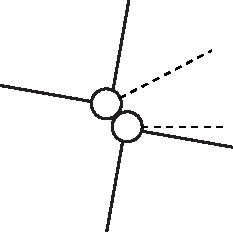
\includegraphics[width=0.22\textwidth]{%
gesamttex/edit_VIII,3/images/LH_37_05_096-099_d2_098r.pdf%
}
\hfill%
}
%
\vspace{0.5em}
\centerline{%
\hfill
\lbrack\textit{Fig.~1}\rbrack \hspace*{45mm}
\lbrack\textit{Fig.~2}\rbrack
\hfill%
}
% \newpage%
\vspace{1em}
%
\pstart
 Porro in directo concursu%
\protect\index{Sachverzeichnis}{concursus directus} etiam alia notari possunt, ut celeritatem respectivam\protect\index{Sachverzeichnis}{celeritas respectiva} semper manere eandem, seu corpora eadem celeritate qua ad se accessere ante ictum,%
\protect\index{Sachverzeichnis}{ictus} ea etiam a se recedere post ictum.\protect\index{Sachverzeichnis}{ictus} Sed hoc quatenus in aliis casibus servari possit, amplius dispiciendum  
%
\edlabel{37_05_096-099_5a}%
\edtext{}{%
{\xxref%
{37_05_096-099_5a}{37_05_096-099_5b}}%
\lemma{est}%
\Bfootnote{%
\textit{(1)}~, tantum enim consequentia est duarum praecedentium regularum quae in casu directi concursus corporum locum habet \textit{(2)}~. Nunc~\textit{L}}}%
est.
\pend
%
\pstart
Nunc%
\edlabel{37_05_096-099_5b}
%
 videamus quid fieri debeat in casu concursus obliqui%
\protect\index{Sachverzeichnis}{concursus obliquus} duorum corporum%
\protect\index{Sachverzeichnis}{concursus obliquus duorum corporum} et  
%
\edtext{quatenus locum}{%
\lemma{quatenus}%
\Bfootnote{\textit{(1)}~interpretatione circa adhibita \textit{(2)}~locum~\textit{L}}} ibi habeat 
%
\edtext{tertia observatio.}{%
\lemma{}%
\Afootnote{\textit{Am Rand, bezogen auf} tertia observatio:\enskip NB Deprehendo eam ibi quoque prorsus succedere.}}  
%
Concursum autem obliquum\protect\index{Sachverzeichnis}{concursus obliquus} 
%
\edtext{voco duorum}{%
\lemma{voco}%
\Bfootnote{%
\textit{(1)}~, cum in momento concursus %
\textit{(2)}~duorum~\textit{L}}}
%
globorum,%
\protect\index{Sachverzeichnis}{globus}%
\protect\index{Sachverzeichnis}{concursus obliquus duorum globorum}  
%
(de his enim nunc tantummodo agemus) cum in momento concursus%
\protect\index{Sachverzeichnis}{momentum concursus} linea ducta per centra%
\protect\index{Sachverzeichnis}{linea per centra} globorum
%
concurrentium angulum faciat ad lineam %
\edtext{qua alter}{%
\lemma{qua}%
\Bfootnote{%
\textit{(1)}~alterum %
\textit{(2)}~alter~\textit{L}}}
%
eorum (vel lineas quibus uterque) movetur. 
\pend
% 
%
\vspace{2.0em} %%%%%%%% Diagramme 3-4
\centerline{%
\hfill
\includegraphics[width=0.16\textwidth]{%
gesamttex/edit_VIII,3/images/LH_37_05_096-099_d3_098r.pdf%
}%
\hfill%
\includegraphics[width=0.13\textwidth]{%
gesamttex/edit_VIII,3/images/LH_37_05_096-099_d4_098r.pdf%
}
\hfill%
} %
\vspace{0.5em}
\centerline{%
\hfill
\lbrack\textit{Fig.~3}\rbrack \hspace*{45mm}
\lbrack\textit{Fig.~4}\rbrack
\hfill%
}
% \newpage%
\vspace{1.5em}
%
\pstart
 Sint duo mobilia\protect\index{Sachverzeichnis}{mobile} (globosa\protect\index{Sachverzeichnis}{mobile globosum} hic semper intelligo) \textit{A} motum, et \textit{B} quiescens. %
Status primus\protect\index{Sachverzeichnis}{status primus} \textit{{\scriptsize1}A}, \textit{{\scriptsize1}B}, status in momento concursus%
\protect\index{Sachverzeichnis}{momentum concursus} \textit{{\scriptsize2}A}, \textit{{\scriptsize2}B}. Coincidunt autem \textit{{\scriptsize1}B} et \textit{{\scriptsize2}B}, quia \textit{B} quiescit. Coincidunt et  
%
\edtext{\textit{{\scriptsize2}B}, \textit{{\scriptsize2}A} si}{%
\lemma{\textit{{\scriptsize2}B}, \textit{{\scriptsize2}A}}%
\Bfootnote{\textit{(1)}~quia \textit{(2)}~uti \textit{(3)}~si~\textit{L}}} considerentur corpora ut  
%
\edtext{puncta, ut rem simplicissime tractemus. Locus centri}{%
\lemma{puncta,}%
\Bfootnote{\textit{(1)}~nulla \textit{(2)}~ut \textit{(a)}~simplicissimos casus primum defin \textit{(b)}~rem simplicissime \textit{(aa)}~co \textit{(bb)}~tractemus. \textit{(aaa)}~Centrum \textit{(bbb)}~Locus centri~\textit{L}}}
%
gravitatis%
\protect\index{Sachverzeichnis}{centrum gravitatis} in primo statu%
\protect\index{Sachverzeichnis}{status primus} \textit{{\scriptsize1}C}, in secundo%
\protect\index{Sachverzeichnis}{status secundus} \textit{{\scriptsize2}C} coincidens cum \textit{{\scriptsize2}A{\scriptsize2}B}, jungatur   
%
\edtext{recta \textit{{\scriptsize1}C{\scriptsize2}C} producaturque}{%
\lemma{recta \textit{{\scriptsize1}C{\scriptsize2}C}}%
\Bfootnote{\textit{(1)}~et \textit{(2)}~producaturque~\textit{L}}}
%
usque in \textit{{\scriptsize3}C}, sic ut \textit{{\scriptsize1}C{\scriptsize2}C}, et \textit{{\scriptsize2}C{\scriptsize3}C} sint aequales. Tertius ergo status%
\protect\index{Sachverzeichnis}{status tertius} nempe post  
%
\edtext{ictum%
\protect\index{Sachverzeichnis}{ictus} (\protect\vphantom)sumto}{%
\lemma{ictum}%
\Bfootnote{%
\textit{(1)}~, posito %
\textit{(2)}~(\protect\vphantom)sumto~\textit{L}}}
%
scilicet aequali temporis intervallo  
%
\edtext{inter statum 1 et 2}{%
\lemma{inter}%
\Bfootnote{\textit{(1)}~1 et 2 quod et inter 2 et 3 status \textit{(2)}~statum 1 et 2~\textit{L}}}  
%
 atque inter statum 2 et 3\vphantom() centri gravitatis%
\protect\index{Sachverzeichnis}{centrum gravitatis} erit ut sit in loco \textit{{\scriptsize3}C}. Si jam consideremus potentiam\protect\index{Sachverzeichnis}{potentia} et directionem \textit{{\scriptsize1}A{\scriptsize2}A}, compositam%
\protect\index{Sachverzeichnis}{potentia composita}%
\protect\index{Sachverzeichnis}{directio composita} ex duabus \textit{{\scriptsize1}AE}, et \textit{E{\scriptsize2}A} 
(\protect\vphantom)nam et hac compositione motuum\protect\index{Sachverzeichnis}{compositio motuum} absolvitur motus per diagonalem,%
\protect\index{Sachverzeichnis}{diagonalis} et ob angulum ad \textit{E} rectum tantum potest \textit{{\scriptsize1}AE} et \textit{E{\scriptsize2}A} simul, quantum \textit{{\scriptsize1}A} 
%
\edtext{\textit{{\scriptsize2}A}\protect\vphantom() perinde}{%
\lemma{\textit{{\scriptsize2}A}\protect\vphantom()}%
\Bfootnote{\textit{(1)}~. Hinc \textit{(2)}~perinde~\textit{L}}} erit, ac si \textit{{\scriptsize1}A} incurrat in 
%
\edtext{\lbrack\textit{B}\rbrack}{%
\lemma{}%
\Bfootnote{%
\textit{E} %
\textit{L ändert~Hrsg.}}}
%
directe velocitate et  
%
\edtext{directione \textit{E{\scriptsize2}A}}{%
\lemma{directione}%
\Bfootnote{\textit{(1)}~\textit{{\scriptsize1}A} \textit{(2)}~\textit{E{\scriptsize2}A}~\textit{L}}}, atque interim pergat celeritate et directione  
%
\edtext{\textit{{\scriptsize1}AE}, itaque in casu}{%
\lemma{\textit{{\scriptsize1}AE},}%
\Bfootnote{\textit{(1)}~ergo si \textit{(2)}~itaque in casu \textit{(3)}~itaque in casu~\textit{L}}} eo quo \textit{A} incurrens in \textit{B}, celeritate et directione \textit{E{\scriptsize2}A}, quiesceret\lbrack,\rbrack\  
%
\edtext{quod fit in casu aequalitatis}{%
\lemma{}%
\Bfootnote{quod fit in casu aequalitatis \textit{erg.~L}}}, etiam hic quiescit quoad hanc directionem; eamque totam transfert in \textit{B}, tantum  
%
\edtext{ergo in producta}{%
\lemma{ergo}%
\Bfootnote{\textit{(1)}~celeritate \textit{(2)}~in producta~\textit{L}}} \textit{E{\scriptsize2}A} sumatur \textit{{\scriptsize2}B{\scriptsize3}B} aequ.\ \textit{E{\scriptsize2}A}, et quia directioni \textit{{\scriptsize1}AE} %
concursus\protect\index{Sachverzeichnis}{concursus} non est  
%
\edtext{contrarius, manet}{%
\lemma{contrarius,}%
\Bfootnote{\textit{(1)}~sumatur \textit{(2)}~manet~\textit{L}}} integra, ac proinde sumatur \textit{{\scriptsize2}A{\scriptsize3}A} aequalis et parallela ipsi  
%
\edtext{\textit{{\scriptsize1}A}\lbrack \textit{E}\rbrack}{%
\lemma{}%
\Bfootnote{\textit{{\scriptsize1}A{\scriptsize2}E} \textit{L ändert Hrsg.}}}. Ita patet  
%
\edtext{pariter et eandem}{%
\lemma{pariter}%
\Bfootnote{\textit{(1)}~centri gravitatis seu c \textit{(2)}~et eandem~\textit{L}}}  
%
directionem totalem,%
\protect\index{Sachverzeichnis}{directio totalis} et eandem potentiam%
\protect\index{Sachverzeichnis}{potentia} conservari. Sed et si celeritatem respectivam%
\protect\index{Sachverzeichnis}{celeritas respectiva} sumamus in  
%
\edtext{recta \textit{EB}}{%
\lemma{recta}%
\Bfootnote{\textit{(1)}~\textit{E{\scriptsize2}A} \textit{(2)}~\textit{EB} \textit{(3)}~\textit{EB}~\textit{L}}} servabitur et ipsa. Quae etiam suo modo locum habebunt si corpora\protect\index{Sachverzeichnis}{corpora inaequalia} sint inaequalia  
%
\edtext{amboque moveri ponantur}{%
\lemma{}%
\Bfootnote{amboque moveri ponantur \textit{erg.~L}}}.%
\edtext{}{% %TRICK für Diagramm 5
\lemma{\hspace*{1,6mm}%
\lbrack\textit{Fig.~5}\rbrack%
}\killnumber%
\Cfootnote{%
Ein gestrichener Entwurf zum Diagramm wird nicht wiedergegeben.%
}}
\pend
%
\vspace{1.0em} %%%%%%%%% Diagramm 5
\centerline{%
\includegraphics[width=0.28\textwidth]{%
gesamttex/edit_VIII,3/images/LH_37_05_096-099_d5_098r.pdf%
}} 
\vspace{0.5em}
\centerline{%
\lbrack\textit{Fig.~5}\rbrack%
}
% \newpage%
\vspace{1.0em}
%
\pstart
Cum autem navis%
\protect\index{Sachverzeichnis}{navis} suppositione%
\protect\index{Sachverzeichnis}{suppositio navis}  
%
\edtext{adhibita explicari}{%
\lemma{adhibita}%
\Bfootnote{\textit{(1)}~optime \textit{(2)}~explicari~\textit{L}}} 
%
eleganter possit concursus\protect\index{Sachverzeichnis}{concursus directus} corporum directus, tribuendo navi%
\protect\index{Sachverzeichnis}{navis} motum qui est ipsius  
%
\edtext{centri;\protect\index{Sachverzeichnis}{motus centri} videndum}{%
\lemma{centri;}%
\Bfootnote{\textit{(1)}~ea res hoc loco commode succedere \textit{(2)}~ea suppositio hoc loco \textit{(a)}~commodo \textit{(b)}~commode non poterit inservire, \textit{(aa)}~sed fingendum est potius \textit{(aaa)}~navim \textit{(bbb)}~duas \textit{(bb)}~si fingamus \textit{(3)}~videndum~\textit{L}}} 
%
an haec suppositio\protect\index{Sachverzeichnis}{suppositio navis} hic quoque inservire possit, nempe %
motus navis\protect\index{Sachverzeichnis}{motus navis} talis supponendus est,  
%
\edtext{ut}{%
\lemma{}%
\Bfootnote{ut \textit{erg.~L}}} 
%
 corpora ambo existentibus in navi%
\protect\index{Sachverzeichnis}{navis} videantur concurrere celeritatibus directis quae sint reciprocae magnitudinum,%
\protect\index{Sachverzeichnis}{celeritates reciprocae magnitudinum} ita ut ambo quibus venere celeritatibus  
%
\edtext{reflectantur, communi}{%
\lemma{reflectantur,}%
\Bfootnote{\textit{(1)}~navi \textit{(2)}~communi~\textit{L}}} interim motu manente. 
%
 Hoc ut investigemus, sit navis \textit{N} in  
%
\edtext{qua mobilia\protect\index{Sachverzeichnis}{mobile}}{%
\lemma{qua}%
\Bfootnote{\textit{(1)}~corpora \textit{(2)}~mobilia~\textit{L}}} 
%
\textit{A} et \textit{B} concurrant in eadem recta ita ut celeritates \textit{{\scriptsize1}A{\scriptsize2}A} et \textit{{\scriptsize1}B{\scriptsize2}B} sint   
%
\edtext{reciproce ut mobilia,\protect\index{Sachverzeichnis}{mobile}}{%
\lemma{reciproce ut}%
\Bfootnote{\textit{(1)}~corpora \textit{(2)}~mobilia,~\textit{L}}}  
%
videndum an talis possit %
navi\protect\index{Sachverzeichnis}{navis} motus   
%
\edtext{tribui ut concursus}{%
\lemma{tribui ut}%
\Bfootnote{\textit{(1)}~inclinatus \textit{(2)}~concursus~\textit{L}}} 
%
 obliquus\protect\index{Sachverzeichnis}{concursus obliquus} propositus oriatur. Ponamus ergo %
navem\protect\index{Sachverzeichnis}{navis} transferri ex \textit{{\scriptsize1}N} in  
%
\edtext{\textit{{\scriptsize2}N} eo tempore}{%
\lemma{\textit{{\scriptsize2}N}}%
\Bfootnote{\textit{(1)}~patet pro \textit{(2)}~eo tempore~\textit{L}}} quo corpora concurrentia ex statu \textit{{\scriptsize1}A{\scriptsize1}B} veniunt in statum 
%
\edtext{\lbrack\textit{{\scriptsize2}A}\rbrack\textit{{\scriptsize2}B},}{%
\lemma{}%
\Bfootnote{%
\textit{{\scriptsize1}B{\scriptsize2}B} %
\textit{L ändert Hrsg.}}}
%
\edtext{patet lineas absolutas%
\protect\index{Sachverzeichnis}{linea absoluta} (\protect\vphantom)ex linea motus navis%
\protect\index{Sachverzeichnis}{motus navis} et motus privati%
\protect\index{Sachverzeichnis}{motus privatus} compositas\protect\vphantom() fore}{%
\lemma{patet}%
\Bfootnote{\textit{(1)}~lineam \textbar\ qua movetur \textit{gestr.}~\textbar\ %
absolutam (ex \lbrack...\rbrack\ privati compositam) \textit{(2)}~lineas absolutas (ex \lbrack...\rbrack\ compositas) \textit{(a)}~fore qua \textit{(b)}~fore~\textit{L}}} 
%
 ${\scriptstyle \textit{1}}A({\scriptstyle \textit{2}}A$) et ${\scriptstyle \textit{1}}B({\scriptstyle \textit{2}}B$), et post  
%
\edtext{ictum nave}{%
\lemma{ictum}%
\Bfootnote{\textit{(1)}~fore lineas motus \textit{(2)}~nave~\textit{L}}} 
%
 translata  
%
\edtext{in \textit{{\scriptsize3}N} sic ut}{%
\lemma{in \textit{{\scriptsize3}N}}%
\Bfootnote{\textit{(1)}~(\protect\vphantom)suppon \textit{(2)}~con \textit{(3)}~sic ut~\textit{L}}} 
%
 \textit{{\scriptsize1}N}, \textit{{\scriptsize2}N}, \textit{{\scriptsize3}N} cadant in eandem rectam, et \textit{{\scriptsize1}N{\scriptsize2}N}, atque \textit{{\scriptsize2}N{\scriptsize3}N} sint  
%
\edtext{aequales (\protect\vphantom)navis}{%
\lemma{aequales (\protect\vphantom)}%
\Bfootnote{\textit{(1)}~quod \textit{(2)}~navis~\textit{L}}} 
%
enim motum%
\protect\index{Sachverzeichnis}{motus navis} nihilo turbari suppono ab ictibus%
\protect\index{Sachverzeichnis}{ictus} corporum in navi,%
\protect\index{Sachverzeichnis}{navis} praesertim si intelligamus ea tam exigua esse, ut ad navim%
\protect\index{Sachverzeichnis}{navis} nullam notabilem habeant proportionalitatem%
\protect\index{Sachverzeichnis}{proportionalitas}\protect\vphantom() motus  
%
\edtext{absoluti%
\protect\index{Sachverzeichnis}{motus absolutus} mobilium%
\protect\index{Sachverzeichnis}{mobile} post}{%
\lemma{absoluti}%
\Bfootnote{\textit{(1)}~corporu \textit{(2)}~mo \textit{(3)}~mobilium \textit{(a)}~erunt \textit{(b)}~post~\textit{L}}} 
%
ictum%
\protect\index{Sachverzeichnis}{ictus} erunt (${\scriptstyle \textit{2}}A){\scriptstyle \textit{3}}A$, et (${\scriptstyle \textit{2}}B){\scriptstyle \textit{3}}B$\lbrack,\rbrack\ ita ut respectu eorum qui sunt in navi \textit{{\scriptsize1}A} et \textit{{\scriptsize3}A}, itemque \textit{{\scriptsize1}B} et \textit{{\scriptsize3}B} coincidant. Verum hinc patet nisi navis motus%
\protect\index{Sachverzeichnis}{motus navis} talis sit, ut linea \textit{{\scriptsize1}N{\scriptsize2}N{\scriptsize3}N} sit parallela  
%
\edtext{ipsi \textit{H{\scriptsize2}A}}{%
\lemma{ipsi}%
\Bfootnote{\textit{(1)}~\textit{H{\scriptsize2}AB} \textit{(2)}~\textit{H{\scriptsize2}A}~\textit{L}}} 
%
(seu \textit{H{\scriptsize2}B}) viae centri  
%
\edtext{gravitatis%
\protect\index{Sachverzeichnis}{via centri gravitatis} tunc fictione}{%
\lemma{gravitatis}%
\Bfootnote{\textit{(1)}~non posse \textit{(a)}~corpora \textit{(b)}~viam \textit{(c)}~centrum gravitatis commune corporum \textit{(2)}~tunc \textit{(a)}~si \textit{(b)}~fictione~\textit{L}}} 
%
 navis assumta rem non succedere, ita  
%
\edtext{enim centrum commun\lbrack e\rbrack%
\protect\index{Sachverzeichnis}{centrum gravitatis commune} non}{%
\lemma{enim}%
\Bfootnote{\textit{(1)}~centri communis \textit{(2)}~centrum~\textbar\ communis \textit{ändert Hrsg.}~\textbar\ non~\textit{L}}} 
%
 progredietur post ictum%
\protect\index{Sachverzeichnis}{ictus}  
%
\edtext{ea directione}{%
\lemma{ea}%
\Bfootnote{\textit{(1)}~via et \textit{(2)}~directione~\textit{L}}} 
%
 et celeritate qua ante ictum\protect\index{Sachverzeichnis}{ictus}. Ita videmus in figura, si \textit{H} sit centrum  
%
\edtext{gravitatis%
\protect\index{Sachverzeichnis}{centrum gravitatis} id}{%
\lemma{gravitatis}%
\Bfootnote{\textit{(1)}~id centr \textit{(2)}~id~\textit{L}}}
 %
post ictum fore $(H)$\lbrack,\rbrack\ sed $H.({\scriptstyle \textit{2}}A).(H)$ non esse  
%
\edtext{rectam. Alioqui}{%
\lemma{rectam.}%
\Bfootnote{\textit{(1)}~Ita enim $(H)$ caderet \textit{(2)}~Alioqui~\textit{L}}} si recta $H({\scriptstyle \textit{2}}A)$ esset continuanda, centrum gr.\ veniret in \textit{K} et proinde propius accederet ad \textit{{\scriptsize3}A}, cum   
%
\edtext{tamen propius debeat}{%
\lemma{tamen propius}%
\Bfootnote{\textit{(1)}~deberet \textit{(2)}~debeat~\textit{L}}} esse ad \textit{{\scriptsize3}B}, nempe in $(H)$ uti \textit{H} propius fuit ad  
%
\edtext{\textit{{\scriptsize1}B}. Attamen}{%
\lemma{\textit{{\scriptsize1}B}.}%
\Bfootnote{\textit{(1)}~Tantum \textit{(2)}~Attamen~\textit{L}}} si navem ipsam consideremus ut tertium corpus, verum  
%
\edtext{nihilominus manet,}{%
\lemma{nihilominus}%
\Bfootnote{\textit{(1)}~nave \textit{(2)}~manet,~\textit{L}}} 
%
omnium viam centri gravitatis\protect\index{Sachverzeichnis}{via centri gravitatis} manere, nam revera ob motum corporum  
%
\edtext{in navi in}{%
\lemma{}%
\Bfootnote{%
in navi \textbar\ motus navis \textit{streicht Hrsg.}~\textbar\ %
in~\textit{L}}}
%
\edtext{hoc casu, si motus navis%
\protect\index{Sachverzeichnis}{motus navis} sit obliquus, ipse}{%
\lemma{hoc}%
\Bfootnote{\textit{(1)}~casu obliqui mo \textit{(2)}~casu, si motus navis sit obliquus \textit{(a)}~ad m \textit{(b)}~, ipse~\textit{L}}} motus navis\protect\index{Sachverzeichnis}{navis} nonnihil movebitur, quia partium eodem tendentium quantitas progressus augetur et  
%
\edtext{imminuitur, quae}{%
\lemma{imminuitur,}%
\Bfootnote{\textit{(1)}~quod \textit{(2)}~quae~\textit{L}}} 
%
tamen difficultas in Hypothesi directi concursus\protect\index{Sachverzeichnis}{concursus directus} cessare videtur. Itaque ratiociniis navis considerationi%
\protect\index{Sachverzeichnis}{consideratio navis} superstructis, atque  
%
\edtext{motu\lbrack u\rbrack m}{%
\lemma{}%
\Bfootnote{motum \textit{L ändert~Hrsg.}}} compositionibus\lbrack,\rbrack%
\protect\index{Sachverzeichnis}{compositio motuum} non est  
%
\edlabel{37_05_096-099_1a}%
\edtext{fidendum.}{%
{\xxref{37_05_096-099_1a}{37_05_096-099_1b}}%
\lemma{fidendum.}%
\Bfootnote{\textit{(1)}~Vi \textit{(2)}~Itaque navis usu \textit{(3)}~Videamus~\textit{L}}} 
\pend
%
%98v
%
\pstart
 \lbrack98~v\textsuperscript{o}\rbrack\ 
\pend
%
\vspace{2.0em} %%%%%%%% Diagramme 6-7
\centerline{%
\hfill
\includegraphics[width=0.19\textwidth]{%
gesamttex/edit_VIII,3/images/LH_37_05_096-099_d6_098v.pdf%
}%
\hfill%
\includegraphics[width=0.13\textwidth]{%
gesamttex/edit_VIII,3/images/LH_37_05_096-099_d7_098v.pdf%
}
\hfill%
} 
\vspace{0.5em}
\centerline{%
\hfill
\lbrack\textit{Fig.~6}\rbrack \hspace*{45mm}
\lbrack\textit{Fig.~7}\rbrack
\hfill%
}
% \newpage%
\vspace{1.5em}
%
\vspace{2.0em} %%%%%%%% Diagramme 8-9
\centerline{%
\hfill
\includegraphics[width=0.2\textwidth]{%
gesamttex/edit_VIII,3/images/LH_37_05_096-099_d8_098v.pdf%
}%
\hfill%
\includegraphics[width=0.2\textwidth]{%
gesamttex/edit_VIII,3/images/LH_37_05_096-099_d9_098v.pdf%
}
\hfill%
} 
\vspace{0.5em}
\centerline{%
\hfill
\lbrack\textit{Fig.~8}\rbrack \hspace*{45mm}
\lbrack\textit{Fig.~9}\rbrack
\hfill%
}
% \newpage%
\vspace{1.5em}
%
%
\pstart
 Videamus\edlabel{37_05_096-099_1b}
%
quid ex aliis considerationibus circa obliquos concursus\protect\index{Sachverzeichnis}{concursus obliquus} duci possit. Equidem si corpora sint aequalia,%
\protect\index{Sachverzeichnis}{corpora aequalia} et velocitates quoque sint aequales,%
\protect\index{Sachverzeichnis}{velocitates aequales} et lineae motuum\protect\index{Sachverzeichnis}{linea motus} \textit{{\scriptsize1}B{\scriptsize2}B},
%
\edtext{\textit{{\scriptsize1}A{\scriptsize2}A}, eundem}{%
\lemma{\textit{{{\scriptsize1}A\scriptsize2}A},}%
\Bfootnote{\textit{(1)}~eandem \textit{(2)}~eundem~\textit{L}}} angulum faciant ad \textit{{\scriptsize2}B{\scriptsize2}A}, rectam centra mobilium jungentem,%
\protect\index{Sachverzeichnis}{recta centra jungens} manifestum est celeritatibus servatis permutari debere directiones, ita ut \textit{{\scriptsize2}B{\scriptsize3}B} sit parallela ipsi \textit{{\scriptsize1}A{\scriptsize2}A}; et similiter \textit{{\scriptsize2}A{\scriptsize3}A}, ipsi  
%
\edtext{\textit{{\scriptsize1}B{\scriptsize2}B}. Ita}{%
\lemma{\textit{{\scriptsize1}B{\scriptsize2}B}.}%
\Bfootnote{\textit{(1)}~Verum vi \textit{(2)}~Ita~\textit{L}}} 
%
enim servatur pariter %
via centri gravitatis\protect\index{Sachverzeichnis}{via centri gravitatis} et %
potentia\protect\index{Sachverzeichnis}{potentia}. Sed  
%
\edtext{si manente}{%
\lemma{si}%
\Bfootnote{\textit{(1)}~ponente \textit{(2)}~manente~\textit{L}}} corporum aequalitate, velocitates sint inaequales,%
\protect\index{Sachverzeichnis}{velocitates inaequales} videndum an tunc etiam locum habeat permutatio\protect\index{Sachverzeichnis}{permutatio}, ut in concursu directo\protect\index{Sachverzeichnis}{concursus directus}. Et ita videtur. Nam ita \textit{{\scriptsize1}C}\lbrack,\rbrack\textit{{\scriptsize2}C},\textit{{\scriptsize3}C} cadent in eandem rectam, et \textit{{\scriptsize1}C{\scriptsize2}C} erit aeq.\ \textit{{\scriptsize2}C{\scriptsize3}C} et praeterea quia \textit{{\scriptsize2}A{\scriptsize3}A} aequ.\ \textit{{\scriptsize1}B{\scriptsize2}B} et \textit{{\scriptsize1}A{\scriptsize2}A} aequ.\ \textit{{\scriptsize2}B{\scriptsize3}B},  
%
\edtext{etiam potentiarum}{%
\lemma{etiam}%
\Bfootnote{\textit{(1)}~potentiae \textit{(2)}~potentiarum~\textit{L}}} 
%
summa%
\protect\index{Sachverzeichnis}{summa potentiarum} manebit.
Et videtur hoc ipso rem esse determinatam, nec aliter haec duo praestari posse\lbrack,\rbrack\ nam si centro \textit{{\scriptsize3}C}, radio \textit{{\scriptsize3}C{\scriptsize3}A} (\protect\vphantom)aequ.\ \textit{{\scriptsize1}C{\scriptsize1}A} aequ.\ \textit{{\scriptsize1}C{\scriptsize1}B}\lbrack\protect\vphantom()\rbrack\
%
describatur circulus  
%
\edtext{ad cujus}{%
\lemma{ad}%
\Bfootnote{\textit{(1)}~quem \textit{(2)}~cujus~\textit{L}}} 
%
puncta opposita quaesita \textit{{\scriptsize3}A}  
%
\edtext{et \textit{{\scriptsize3}B} ductae}{%
\lemma{et \textit{{\scriptsize3}B}}%
\Bfootnote{\textit{(1)}~ducendae sunt rectae \textit{(2)}~ductae~\textit{L}}}  
%
rectae \edtext{\textit{{\scriptsize2}A{\scriptsize3}A}, \textit{{\scriptsize2}B{\scriptsize3}B}}{%
\lemma{}%
\Bfootnote{\textit{{\scriptsize2}A{\scriptsize3}A}, \textit{{\scriptsize2}B{\scriptsize3}B} \textit{erg.~L}}} sint tales  
%
\edtext{ut summa}{%
\lemma{ut}%
\Bfootnote{\textit{(1)}~quadratum eorum \textit{(2)}~summa~\textit{L}}} 
%
quadratorum%
\protect\index{Sachverzeichnis}{summa quadratorum} ab ipsis sit aequalis  
%
\edtext{datae quantitati}{%
\lemma{datae}%
\Bfootnote{\textit{(1)}~summae \textit{(2)}~quantitati~\textit{L}}}, res opinor non aliter poterit praestari,  
%
\edtext{quam uno}{%
\lemma{quam}%
\Bfootnote{\textit{(1)}~hoc \textit{(2)}~uno~\textit{L}}} determinato modo, at is jam habetur in casu per omnia congruo, cum  
%
\edtext{aequalis}{%
\lemma{aequalis}%
\Bfootnote{\textit{erg.~L}}} circulus esset centro \textit{{\scriptsize1}C} descriptus, ubi  
%
\edtext{similiter quadrata}{%
\lemma{similiter}%
\Bfootnote{\textit{(1)}~\textit{{\scriptsize1}A{\scriptsize2}A} \textit{(2)}~\textit{{\scriptsize2}A{\scriptsize1}A} et \textit{(3)}~quadrata~\textit{L}}} 
%
de \textit{{\scriptsize2}A{\scriptsize1}A} et de \textit{{\scriptsize2}B{\scriptsize1}B} faciebant eandem summam,\protect\index{Sachverzeichnis}{summa quadratorum}
%
 tantum ergo opus est sumere \textit{{\scriptsize3}A{\scriptsize3}C{\scriptsize3}B} parallelam ipsi \textit{{\scriptsize1}A{\scriptsize1}C{\scriptsize1}B}. Hinc autem porro sequitur si \textit{{\scriptsize1}B} et \textit{{\scriptsize2}B} coincidant, seu si \textit{B} quiescat ante ictum\protect\index{Sachverzeichnis}{ictus}, etiam \textit{{\scriptsize2}A{\scriptsize3}A} coincidere seu \textit{A} quiescere  
%
\edlabel{37_05_096-099_4a}%
%
\edtext{}{% 
{\xxref%
{37_05_096-099_4a}{37_05_096-099_4b}}%
\lemma{post ictum.}%
\Bfootnote{%
\textit{(1)}~Verum hinc jam video rem non esse determinatam satis, ex duabus illis regulis de servata simul potentia absoluta et totali directione, nam paulo ante easdem regulas servando aliud pronuntiavimus. Hinc jam consequitur erroneam esse Methodum \textit{(2)}~At diversa est Methodus~\textit{L}}}%
post ictum.
\pend
%
%
\vspace{1.0em} %%%%%%%%% Diagramm 10
\centerline{%
\includegraphics[width=.25\textwidth]{%
gesamttex/edit_VIII,3/images/LH_37_05_096-099_d10_098v.pdf%
}} 
\vspace{0.5em}
\centerline{%
\lbrack\textit{Fig.~10}\rbrack%
}
% \newpage%
\vspace{1em}
%
%
\pstart
At diversa est Methodus%
\edlabel{37_05_096-099_4b}
%
investigandi concursuum obliquorum\protect\index{Sachverzeichnis}{concursus obliquus} effectus ex motuum compositione\protect\index{Sachverzeichnis}{compositio motuum},%
\protect\index{Sachverzeichnis}{methodus investigandi ex compositione motuum} ut si in quiescens \textit{B} incurrat \textit{A} oblique linea  
%
\edtext{\textit{{\scriptsize1}A{\scriptsize2}A} ponamusque}{%
\lemma{\textit{{\scriptsize1}A{\scriptsize2}A}}%
\Bfootnote{\textit{(1)}~si conciperemus \textit{(2)}~ponamusque~\textit{L}}} \textit{A} et \textit{B}  
%
\edtext{aequalia; et concipiamus}{%
\lemma{}%
\Bfootnote{aequalia; \textbar\ et \textit{erg.} \textbar\ concipiamus~\textit{L}}}
%
 motum \textit{{\scriptsize1}A{\scriptsize2}A} compositum%
\protect\index{Sachverzeichnis}{motus compositus} ex motu \textit{{\scriptsize1}AE}, et \textit{E{\scriptsize2}A},  
%
\edtext{ac}{%
\lemma{ac}%
\Bfootnote{\textit{erg.~L}}} post ictum%
\protect\index{Sachverzeichnis}{ictus} sumamus \textit{{\scriptsize2}B{\scriptsize3}B} aequ.\ \textit{E{\scriptsize2}A}, et \textit{{\scriptsize2}A{\scriptsize3}A}  
%
\edtext{aequ.\ \textit{AE}, patet}{%
\lemma{aequ.\ \textit{AE},}%
\Bfootnote{%
\textit{(1)}~dico %
\textit{(2)}~patet~\textit{L}}}
%
hac ratione quidem servari summam  
%
\edtext{potentiarum;%
\protect\index{Sachverzeichnis}{summa potentiarum} sed}{%
\lemma{potentiarum;}%
\Bfootnote{\textit{(1)}~sed non directionem \textbar\ et celeritatem \textit{erg.}~\textbar\ centri gravitatis utique enim \textit{(2)}~sed~\textit{L}}} 
%
 videndum an etiam servetur directio%
\protect\index{Sachverzeichnis}{directio centri gravitatis} et celeritas centri\protect\index{Sachverzeichnis}{celeritas centri gravitatis} gravitatis. Ponamus corpora  
%
\edtext{\textit{A} et \textit{B}}{%
\lemma{}%
\Bfootnote{\textit{A} et \textit{B} \textit{erg.~L}}} tam esse exigua,%
\protect\index{Sachverzeichnis}{corpus exiguum} ut puncta \textit{{\scriptsize2}A}, \textit{{\scriptsize2}B}, adeoque et \textit{{\scriptsize2}C} pro coincidentibus haberi possint; videndum an continuata \textit{{\scriptsize1}C{\scriptsize2}C} bisecet \textit{{\scriptsize3}A{\scriptsize3}B} in  
%
\edtext{\textit{{\scriptsize3}C}, quod}{%
\lemma{\textit{{\scriptsize3}C},}%
\Bfootnote{\textit{(1)}~ita ut \textit{(2)}~quod~\textit{L}}} verum esse patet, est enim \textit{{\scriptsize1}A{\scriptsize2}A} diagonalis\protect\index{Sachverzeichnis}{diagonalis} rectanguli
 \textit{{\scriptsize1}AE{\scriptsize2}A}, ergo et continuata rectanguli  
%
\edtext{\textit{{\scriptsize3}A{\scriptsize2}C{\scriptsize3}B} (\protect\vphantom)priori}{%
\lemma{\textit{{\scriptsize3}A{\scriptsize2}C{\scriptsize3}B}}%
\Bfootnote{\textit{(1)}~erit diagonalis, ergo alte \textit{(2)}~(\protect\vphantom)priori~\textit{L}}} 
%
 per omnia congruentis et deinceps positi\protect\vphantom() erit diagonalis, ergo hujus alteram diagonalem%
\protect\index{Sachverzeichnis}{diagonalis}
%
 \textit{{\scriptsize3}A{\scriptsize3}B} bisecabit. Itaque ut \textit{{\scriptsize1}C} medium ipsius \textit{{\scriptsize1}A{\scriptsize1}B} (seu \textit{{\scriptsize1}A{\scriptsize2}A})
%
 est %
centrum gravitatis\protect\index{Sachverzeichnis}{centrum gravitatis} ipsorum \textit{A} et \textit{B} aequalium in statu 1\textsuperscript{mo},%
\protect\index{Sachverzeichnis}{status primus} ita et \textit{{\scriptsize3}C} medium ipsius \textit{{\scriptsize3}A{\scriptsize3}B} erit centrum%
\protect\index{Sachverzeichnis}{centrum gravitatis} grav.\ aequalium \textit{A} et \textit{B} in statu tertio;%
\protect\index{Sachverzeichnis}{status tertius} et patet \textit{{\scriptsize1}C}, \textit{{\scriptsize2}C}, \textit{{\scriptsize3}C} esse in eadem recta, itemque \textit{{\scriptsize1}C{\scriptsize2}C}, et \textit{{\scriptsize2}C{\scriptsize3}C} esse aequales. 
\pend
% %
\pstart
 Habemus ergo duas diversas conclusiones ex iisdem principiis ductas, unde manifestum est, principia ista duo (potentiae%
\protect\index{Sachverzeichnis}{principium servatae potentiae} et directionis totalis servatae%
\protect\index{Sachverzeichnis}{principium servatae directionis totalis}) non sufficere ad rem penitus determinandam. 
\pend
% %
\pstart
 Videtur autem via ex compositione motuum\protect\index{Sachverzeichnis}{compositio motuum} esse praeferenda, neque rationi%
\protect\index{Sachverzeichnis}{ratio} consentaneum esse, ut \textit{A} incurrens in quiescens \textit{B}, semper eodem modo ab eo sistatur, licet  
%
\edtext{ipsum prope radat}{%
\lemma{ipsum}%
\Bfootnote{\textit{(1)}~radat tantum exigue \textit{(2)}~ver \textit{(3)}~proper \textit{(4)}~prope radat~\textit{L}}} et tantum; et sane generalis mea ratio talia examinandi a posteriori obstat. Nam si angulus \textit{{\scriptsize1}A{\scriptsize2}A{\scriptsize2}B} continue magis ad rectum  
%
\edtext{acceder\lbrack e\rbrack t}{%
\lemma{}%
\Bfootnote{accedert \textit{L ändert Hrsg.}}}, sequeretur nihilominus eundem semper sequi effectum,%
\protect\index{Sachverzeichnis}{effectus} ut tota potentia\protect\index{Sachverzeichnis}{potentia tota} ipsius \textit{A} transferatur in \textit{B}, ergo et in illo casu id fiet, qui indefinitesime differt ab impulsu nullo,%
\protect\index{Sachverzeichnis}{impulsus nullus} cum scilicet angulus a recto indefinitesime differt, aut differentia utcunque parva;%
\protect\index{Sachverzeichnis}{differentia utcunque parva} cum tamen in casu recti prorsus anguli impulsus sit plane nullus,%
\protect\index{Sachverzeichnis}{impulsus nullus} nullaque virium translatio\protect\index{Sachverzeichnis}{translatio virium}. Quod et cum methodo per compositionem motuum%
\protect\index{Sachverzeichnis}{methodus per compositionem motuum} prorsus consentit. Haec ergo praeferenda est. Ex his  
%
\edtext{patet quot modis possit}{%
\lemma{patet}%
\Bfootnote{\textit{(1)}~infinitis modis posse \textit{(2)}~quot modis possit~\textit{L}}} satisfieri duabus regulis servandae potentiae totalis%
\protect\index{Sachverzeichnis}{regula servandae potentiae totalis}%
\protect\index{Sachverzeichnis}{potentia totalis} et servandae directionis totalis.%
\protect\index{Sachverzeichnis}{regula servandae directionis totalis}%
\protect\index{Sachverzeichnis}{directio totalis} Sumto enim \textit{{\scriptsize3}C}, quale ex regula directionis totalis servandae\protect\index{Sachverzeichnis}{regula servandae directionis totalis} determinatur; et centro \textit{{\scriptsize3}C} radio \textit{{\scriptsize3}C{\scriptsize2}C} (aequ \textit{{\scriptsize1}C{\scriptsize2}C}) describendo circulum ad quem ex puncto \textit{{\scriptsize2}C} ducendae sunt duae rectae, quarum potentiae%
\protect\index{Sachverzeichnis}{potentia} simul sunt aequales potentiae%
\protect\index{Sachverzeichnis}{potentia} ipsius \textit{{\scriptsize1}A{\scriptsize2}A}, seu ipsius diametri \textit{{\scriptsize3}A{\scriptsize3}B}. At  
%
\edtext{rectae a circuli puncto uno ad duo alia ductae}{%
\lemma{rectae a}%
\Bfootnote{\textit{(1)}~circulo \textit{(2)}~circuli puncto uno ad duo alia ductae~\textit{L}}}
%
 quarum quadrata simul aequari debent quadrato diametri, duci debent ad duo puncta opposita unius diametri, ergo quot diametri in circulo possunt duci tot modis satisfieri posset\lbrack,\rbrack\ hoc est modis infinitis. Exempli causa \textit{{\scriptsize2}CS} et \textit{{\scriptsize2}CT}, ita ut \textit{B} ex \textit{{\scriptsize2}B} perveniret in \textit{S}, et \textit{A} ex \textit{{\scriptsize2}A} in \textit{T}. Verum ille modus eligendus est, quo motuum compositio%
\protect\index{Sachverzeichnis}{compositio motuum} servatur, ut ostendimus.%
\edtext{}{\killnumber\lemma{\hspace*{1,6mm}%
\lbrack\textit{Fig.~11}\rbrack}% 
\Cfootnote{Die Buchstaben \textit{m} und \textit{n} in der Zeichnung ändert Hrsg.\ nach den Angaben im Text.}}
\pend
%
%
\vspace{1.0em} %%%%%%%%% Diagramm 11
\centerline{%
\includegraphics[width=.6\textwidth]{%
gesamttex/edit_VIII,3/images/LH_37_05_096-099_d11_098v.pdf%
}} 
\vspace{0.5em}
\centerline{%
\lbrack\textit{Fig.~11}\rbrack%
}
% \newpage%
\vspace{1em}
%
\pstart
%
Eidem Methodo insistendo generaliter si sint  
%
\edtext{in rectam \textit{{\scriptsize2}A{\scriptsize2}B}}{%
\lemma{}%
\Bfootnote{in rectam \textit{{\scriptsize2}A{\scriptsize2}B} \textit{erg.~L}}} perpendiculares \textit{{\scriptsize1}AE}, \textit{{\scriptsize1}BF}, \textit{{\scriptsize3}AG},  
%
\edtext{\textit{{\scriptsize3}BH}; erunt aequales}{%
\lemma{\textit{{\scriptsize3}BH};}%
\Bfootnote{\textit{(1)}~et aequalis sit \textit{(2)}~erunt aequales \textbar\ sit \textit{streicht Hrsg.}~\textbar\ \textit{{\scriptsize1}AE}~\textit{L}}} 
%
 \textit{{\scriptsize1}AE} ipsi \textit{{\scriptsize3}AG}, et \textit{{\scriptsize1}BF} ipsi \textit{{\scriptsize3}BH}, at \textit{{\scriptsize2}AG} ipsi \textit{{\scriptsize2}BF}, et \textit{{\scriptsize2}BH} ipsi \textit{{\scriptsize2}AE}, quo posito debet   
%
\edtext{recta \textit{{\scriptsize1}C{\scriptsize2}C{\scriptsize3}C} quae}{%
\lemma{recta}%
\Bfootnote{\textit{(1)}~\textit{{\scriptsize1}C{\scriptsize2}C} producta \textit{(a)}~secare \textit{(b)}~bisecare \textit{(2)}~\textit{{\scriptsize1}C{\scriptsize2}C{\scriptsize3}C} quae~\textit{L}}} 
%
bisecat \textit{{\scriptsize1}A{\scriptsize1}B}, etiam producta bisecare \textit{{\scriptsize3}A{\scriptsize3}B}\lbrack,\rbrack\ quod est theorema Geometricum satis singulare.\protect\index{Sachverzeichnis}{theorema Geometricum satis singulare}  
%
Sed tamen examinandum adhuc ut de successu simus securiores.
\pend
%
\pstart
${\scriptstyle \textit{2}}CE={\scriptstyle \textit{2}}CH$ sit \textit{e}\lbrack,\rbrack\ ${\scriptstyle \textit{2}}CF={\scriptstyle \textit{2}}CG$ sit \textit{f}; et \textit{{\scriptsize1}BF} seu \textit{{\scriptsize3}BH} sit \textit{h} et \textit{{\scriptsize1}AE} seu \textit{{\scriptsize3}AG} sit \textit{g}. 
%
\textit{FE} seu \textit{HG} erit $e+f={\scriptstyle \textit{1}}AM=$  
%
\edtext{\textit{{\scriptsize3}AN}, et}{%
\lemma{\textit{{\scriptsize3}AN},}%
\Bfootnote{et \textit{erg.~L}}} 
%
${\scriptstyle \textit{1}}A{\scriptstyle \textit{2}}A=\sqrt{ee+gg}$ et ${\scriptstyle \textit{1}}B{\scriptstyle \textit{2}}B=\sqrt{ff+hh}$ et 
\rule[0cm]{0mm}{14pt}${\scriptstyle \textit{2}}A{\scriptstyle \textit{3}}A=\sqrt{ff+gg}$ et ${\scriptstyle \textit{2}}B{\scriptstyle \textit{3}}B=$ 
%
\edtext{$\sqrt{ee+hh}$. \textit{{\scriptsize1}A{\scriptsize1}B}}{%
\lemma{$\sqrt{ee+hh}$.}%
\Bfootnote{%
\textit{(1)}~${\scriptstyle \textit{1}}B{\scriptstyle \textit{1}}A=$ \textit{(2)}~\textit{{\scriptsize1}A{\scriptsize1}B}~\textit{L}}}
%
\rule[0cm]{0mm}{14pt}\edtext{$(=\sqrt{\protect\boxed{\phantom{2}}\;{\scriptstyle \textit{1}}BM+\protect\boxed{\phantom{2}}\;M{\scriptstyle \textit{1}}A})$}{%
\lemma{}%
\Bfootnote{$(=\sqrt{\protect\boxed{\phantom{2}}\;{\scriptstyle \textit{1}}BM+\protect\boxed{\phantom{2}}\;M{\scriptstyle \textit{1}}A})$ \textit{erg.~L}}}%
%
$\;={\scriptstyle \textit{3}}A{\scriptstyle \textit{3}}B$ 
%
\edtext{$(=\sqrt{\protect\boxed{\phantom{2}}\;{\scriptstyle \textit{3}}BN+\protect\boxed{\phantom{2}}\;N{\scriptstyle \textit{3}}A})$}{%
\lemma{$(=\sqrt{\protect\boxed{\phantom{2}}\;{\scriptstyle \textit{3}}BN+\protect\boxed{\phantom{2}}\;N{\scriptstyle \textit{3}}A})$}%
\Bfootnote{\textit{erg.~L}}}%
%
$\;=\sqrt{\protect\boxed{2}\;\overline{e+f}+\protect\boxed{2}\;\overline{h-g}}$. 
%
\edtext{Ubi illud memorabile oritur, quod}{%
\lemma{}%
\Afootnote{\textit{Am Rand}:\enspace seu =}}  
%
\edtext{ut}{%
\lemma{}%
\Bfootnote{ut \textit{erg.~L}}} 
%
\rule[0cm]{0mm}{10pt}hactenus semper sive in recto%
\protect\index{Sachverzeichnis}{concursus rectus}%
\protect\index{Sachverzeichnis}{concursus rectus duorum} sive in obliquo duorum concursu,%
\protect\index{Sachverzeichnis}{concursus obliquus}%
\protect\index{Sachverzeichnis}{concursus obliquus duorum} ita et nunc in generali ista obliqui concursus  
%
\edtext{aequalium%
\protect\index{Sachverzeichnis}{concursus obliquus aequalium}}{%
\lemma{}%
\Bfootnote{aequalium \textit{erg.~L}}} 
%
 determinatione deprehenditur eandem esse distantiam mobilium  
%
\edtext{aequali temporis}{%
\lemma{aequali}%
\Bfootnote{\textit{(1)}~tempore su \textit{(2)}~temporis~\textit{L}}} 
%
 intervallo sumto ante ictum%
\protect\index{Sachverzeichnis}{ictus} et post ictum, seu eandem manere celeritatem respectivam\protect\index{Sachverzeichnis}{celeritas respectiva}, sive eandem esse celeritatem recessus\protect\index{Sachverzeichnis}{celeritas recessus} post ictum%
\protect\index{Sachverzeichnis}{ictus} quae fuit appropinquationis\protect\index{Sachverzeichnis}{celeritas appropinquationis}   
%
\edtext{ante ictum. Videamus}{%
\lemma{ante ictum.}%
\Bfootnote{\textit{(1)}~Hinc etiam cum figura \textit{{\scriptsize3}A{\scriptsize3}G{\scriptsize2}CH{\scriptsize3}B} \textit{(a)}~non ali \textit{(b)}~per omnia congruat figurae \textit{{\scriptsize1}A} \textit{(2)}~Videamus~\textit{L}}} 
%
 tantum de \textit{C}. Per \textit{{\scriptsize3}C} ducamus $45.{\scriptstyle \textit{3}}C.6$ parallelam et aequalem ipsi \textit{HG} vel \textit{FE}, et per 
%
\edtext{\textit{{\scriptsize1}C} ducamus $78.{\scriptstyle \textit{1}}C.9$}{%
\lemma{\textit{{\scriptsize1}C} ducamus}%
\Bfootnote{\textit{(1)}~$789.{\scriptstyle \textit{1}}C.$ \textit{(2)}~$78.{\scriptstyle \textit{1}}C.9$~\textit{L}}} 
%
 aequalem et parallelam
%99r
\lbrack99~r\textsuperscript{o}\rbrack\ ipsi \textit{FE} seu \textit{HG}. Primum manifestum est triangulum ${\scriptstyle \textit{3}} 
%
BN{\scriptstyle \textit{3}}A$ congruere triangulo \textit{{\scriptsize1}BM{\scriptsize1}A}, est enim utrumque rectangulum, et  
%
altitudines atque bases sunt aequales (\protect\vphantom)adeoque ut jam quoque notavimus et Hypotenusae  
%
\textit{{\scriptsize1}A{\scriptsize1}B} ipsi \textit{{\scriptsize3}A{\scriptsize3}B};\protect\vphantom() ac proinde et aequiangulum erit. 
%
 Hinc si sumamus \textit{{\scriptsize1}C} medium in \textit{{\scriptsize1}A{\scriptsize1}B}, et \textit{{\scriptsize3}C}  
%
medium in \textit{{\scriptsize3}A{\scriptsize3}B}. Manifestum est et \textit{{\scriptsize3}C} fore medium ipsius 46,  
%
ut \textit{{\scriptsize1}C} ipsius 79. Et quia 45 quoque $={\scriptstyle \textit{2}}CH={\scriptstyle \textit{2}}CE=78$.  
%
Hinc $5.{\scriptstyle \textit{3}}C=4.{\scriptstyle \textit{3}}C-\edtext{\lbrack45\rbrack$}{%
\lemma{$5.{\scriptstyle \textit{3}}C$}%
\Bfootnote{\textit{L ändert Hrsg.}}} 
%
$=7.{\scriptstyle \textit{1}}C-78=8.{\scriptstyle \textit{1}}C$. Rursus $4.{\scriptstyle \textit{3}}B=9.{\scriptstyle \textit{1}}B$, (\protect\vphantom)quia idem angulus  
%
\edtext{$9.{\scriptstyle \textit{1}}B{\scriptstyle \textit{1}}C$ idem}{%
\lemma{$9.{\scriptstyle \textit{1}}B{\scriptstyle \textit{1}}C$}%
\Bfootnote{\textit{(1)}~aequ.\ \textit{(2)}~idem~\textit{L}}} est angulo $4.{\scriptstyle \textit{3}}B.{\scriptstyle \textit{3}}C$ unde haec duo triangula rectangula  
%
\edtext{cum bases}{%
\lemma{cum}%
\Bfootnote{\textit{(1)}~altitudinem \textit{(2)}~bases~\textit{L}}} 
%
 habeant aequales $4.{\scriptstyle \textit{3}}C=9.{\scriptstyle \textit{1}}C$ etiam altitudines habebunt aequales\protect\vphantom().
%
Ergo et ${\scriptstyle \textit{2}}C.5={\scriptstyle \textit{2}}C.8$. Cum ergo triangula rectangula ${\scriptstyle \textit{2}}C.8.{\scriptstyle \textit{1}}C$ et ${\scriptstyle \textit{2}}C.5.{\scriptstyle \textit{3}}C$ habeant bases et altitudines aequales, habebunt et aequales Hypotenusas \textit{{\scriptsize2}C{\scriptsize1}C} et \textit{{\scriptsize2}C{\scriptsize3}C}, et praeterea puncta \textit{{\scriptsize1}C}, \textit{{\scriptsize2}C}, \textit{{\scriptsize3}C} cadent in eandem rectam quod erat ostendendum. 
\pend
% 
%
\vspace{2.0em} %%%%%%%%% Diagramm 12
\centerline{%
\includegraphics[width=0.21\textwidth]{%
gesamttex/edit_VIII,3/images/LH_37_05_096-099_d12_099r.pdf%
}} 
\vspace{0.5em}
\centerline{%
\lbrack\textit{Fig.~12}\rbrack%
}
% \newpage%
\vspace{1.5em}
%
%
\pstart
 Ad leges Tabulae Globivolvae\protect\index{Sachverzeichnis}{Tabula Globivolva},  
%
quam Germani\protect\index{Sachverzeichnis}{Germani} trucktafel\protect\index{Sachverzeichnis}{trucktafel},  
%
Galli\protect\index{Sachverzeichnis}{Galli} billard\protect\index{Sachverzeichnis}{Billard} 
%
 vocant, definiendas tantum opus est considerare  
%
angulos incidentiae\protect\index{Sachverzeichnis}{angulus incidentiae}  
%
et reflexionis\protect\index{Sachverzeichnis}{angulus reflexionis}  
%
esse aequales, et tenere legem%
\protect\index{Sachverzeichnis}{lex de effectibus incursus} quam supra attulimus de  
%
\edtext{effectibus incursus%
\protect\index{Sachverzeichnis}{incursus}}{%
\lemma{effectibus}%
\Bfootnote{\textit{(1)}~concursus \textit{(2)}~incursus~\textit{L}}} 
%
 aequalium%
\protect\index{Sachverzeichnis}{incursus aequalium} quorum unum quiescit, sive is sit obliquus%
\protect\index{Sachverzeichnis}{incursus obliquus} sive rectus%
\protect\index{Sachverzeichnis}{incursus rectus}. Itaque si a reflexione  
%
quaeram attingere punctum sive illa sit simplex%
\protect\index{Sachverzeichnis}{reflexio simplex} sive repetita,%
\protect\index{Sachverzeichnis}{reflexio repetita}  
%
tantum opus est observare aequalitatem angulorum.  
%
Atque hoc inprimis utile est  
%
\edtext{consider\lbrack ar\rbrack e}{%
\lemma{}%
\Bfootnote{considere \textit{L ändert Hrsg.}}} 
%
 ad faciendam Romanam ut nostri vocant, id  
%
est, ut per reflexionem simplicem%
\protect\index{Sachverzeichnis}{reflexio simplex} vel etiam duplicem,%
\protect\index{Sachverzeichnis}{reflexio duplex} globulus%
\protect\index{Sachverzeichnis}{globulus} portam trajiciat. 
Ut vero alterius globum%
\protect\index{Sachverzeichnis}{globus} in foramen impellam hoc sine consideratione reflexionis%
\protect\index{Sachverzeichnis}{reflexio} effici potest, ex lege  
%
concursus obliqui aequalium\protect\index{Sachverzeichnis}{concursus obliquus aequalium}\protect\index{Sachverzeichnis}{lex concursus obliqui aequalium}, quorum alterum quiescit, supra stabilita. Nempe meus  
%
\edtext{%
globus\protect\index{Sachverzeichnis}{globus} \textit{A} sit in loco}{%
\lemma{globus}%
\Bfootnote{\textit{(1)}~sit \textit{(2)}~\textit{A} in statu \textit{(3)}~\textit{A} sit in loco~\textit{L}}} 
%
 \textit{{\scriptsize1}A}, tuus \textit{B} in loco \textit{{\scriptsize1}B}, et volo tum ita impellere ut eat versus \textit{{\scriptsize2}B} 
%
 ibique cadat in foramen. Debeo lineam \textit{{\scriptsize1}A{\scriptsize2}A} sumere talem, ut in momento ictus\protect\index{Sachverzeichnis}{momentum ictus} 
%
 \textit{{\scriptsize2}B}, \textit{{\scriptsize1}B}, et \textit{{\scriptsize2}A} cadant in eandem rectam, 
%
 seu ut recta per centra globorum in %
momento concursus\protect\index{Sachverzeichnis}{momentum concursus}  
%
\edtext{transiens producta}{%
\lemma{transiens}%
\Bfootnote{\textit{(1)}~tendat ad locum \textit{(2)}~producta~\textit{L}}}
%
ad locum illum  
%
\edtext{\textit{{\scriptsize2}B}}{%
\lemma{\textit{{\scriptsize2}B}}%
\Bfootnote{%
\textit{erg.~L}}}
%
tendat.
\pend
% %
\pstart
 Posset Tabula  
%
\edtext{Globivolva\protect\index{Sachverzeichnis}{Tabula Globivolva} numeris}{%
\lemma{Globivolva}%
\Bfootnote{\textit{(1)}~gradibus \textit{(2)}~numeris~\textit{L}}} distingui, vel etiam  
%
\edtext{possent aliqu\lbrack ae\rbrack\ notari partes}{%
\lemma{possent}%
\Bfootnote{\textit{(1)}~gradus \textbar\ aliqui \textit{erg.}~\textbar\ \textit{(2)}~\textbar~aliqui \textit{ändert Hrsg.}~\textbar\ notari partes~\textit{L}}}
%
 aequales in bacillo,%
\protect\index{Sachverzeichnis}{bacillus} qui ad mensurandum  
%
\edtext{inserviret, idque}{%
\lemma{inserviret}%
\Bfootnote{\textit{(1)}~, pr \textit{(2)}~; atque ita \textit{(3)}~, idque~\textit{L}}} 
%
 usui esse posset non in ludendo tantum sed et potius in regulis 
%
 motuum\protect\index{Sachverzeichnis}{regulae motuum} definiendis. Poterit etiam  
%
ope speculi plani%
\protect\index{Sachverzeichnis}{speculum planum} ex polito metallo, quod esset in bacilli%
\protect\index{Sachverzeichnis}{bacillus} extremo, quaeri  
%
\edtext{punctum in pariete Tabulae%
\protect\index{Sachverzeichnis}{Tabula Globivolva} in quo ex globulo%
\protect\index{Sachverzeichnis}{globulus}}{%
\lemma{punctum}%
\Bfootnote{\textit{(1)}~ex \textit{(2)}~\textbar\ in pariete Tabulae \textit{erg.}~\textbar\ in quo ex \textit{(a)}~sphae \textit{(b)}~globulo~\textit{L}}} 
%
meo globulus alterius videri posset per reflexionem.%
\protect\index{Sachverzeichnis}{reflexio}  
%
\edlabel{37_05_096-099_6a}%	
Artifices in ludo globivolvo%
\protect\index{Sachverzeichnis}{ludus globivolvus} exercitati aliquando ponunt nummum%
\protect\index{Sachverzeichnis}{nummus}  
%
sub aliquo
%
globo,%
\protect\index{Sachverzeichnis}{globus} et deinde alterum globum ita impellunt in priorem, ut priore pulso posterior super  
%
\edtext{ipso nummo%
\protect\index{Sachverzeichnis}{nummus} sese}{%
\lemma{ipso}%
\Bfootnote{\textit{(1)}~numero \textit{(2)}~nummo \textit{(a)}~qui \textit{(b)}~sese~\textit{L}}} 
%
collocet in prioris locum.\edlabel{37_05_096-099_6b} 
%
 Habent etiam artem ita impellendi globum%
\protect\index{Sachverzeichnis}{globus} alterius, ut evolet ex tabula%
\protect\index{Sachverzeichnis}{Tabula Globivolva} per arcum, 
%
 sed ea ratione suummet globulum%
\protect\index{Sachverzeichnis}{globulum} huic periculo etiam exponunt, ut ipse potius exiliat. Expellere autem globum  
%
adversarii tum maxime possunt, cum ipse prope portulam requiescit. Quorum omnium pro re nata 
%
non difficulter reddetur ratio.%
\pend
% 
%
\vspace{2.0em} %%%%%%%%% Diagramm 13
\centerline{%
\includegraphics[width=.4\textwidth]{%
gesamttex/edit_VIII,3/images/LH_37_05_096-099_d13_099r.pdf%
}} 
\vspace{0.5em}
\centerline{%
\lbrack\textit{Fig.~13}\rbrack%
}
% \newpage%
\vspace{1.5em}
%
\pstart
\edtext{}{%		% TRICK für Fig. 13
\lemma{\hspace*{1,6mm}%
\lbrack\textit{Fig.~13}\rbrack%
}\killnumber%
\Cfootnote{%
Ein gestrichener Entwurf zum Diagramm wird nicht wiedergegeben.%
}}%
%
Si tam corpora\protect\index{Sachverzeichnis}{corpora inaequalia} quam celeritates%
\protect\index{Sachverzeichnis}{celeritates inaequales} sint inaequales eaedem plane succedunt demonstrationes.  
%
\edtext{Sint ex \textit{{\scriptsize1}A}, \textit{{\scriptsize1}B}, \textit{{\scriptsize3}A}, \textit{{\scriptsize3}B} perpendiculares \textit{{\scriptsize1}A{\scriptsize1}E}, aequal. \textit{{\scriptsize3}A{\scriptsize3}E},}{%
\lemma{Sint}%
\Bfootnote{\textit{(1)}~perpendiculares \textit{(2)}~ex \textit{{\scriptsize1}A}, \textit{{\scriptsize1}B}, \textit{{\scriptsize3}A}, \textit{{\scriptsize3}B} perpendiculares \textit{{\scriptsize1}A{\scriptsize1}E}, \textit{(a)}~\textit{{\scriptsize1}B{\scriptsize1}F}, \textit{{\scriptsize3}A{\scriptsize3}E}, \textit{{\scriptsize3}B{\scriptsize3}F} \textit{(b)}~aequal. \textit{{\scriptsize3}A{\scriptsize3}E},~\textit{L}}} 
%
et \textit{{\scriptsize1}B{\scriptsize1}F} aequ.\ \textit{{\scriptsize3}B{\scriptsize3}F} et sit  
%
\edtext{\textit{{\scriptsize3}E{\scriptsize3}F} aequ.\ \lbrack\textit{{\scriptsize1}E{\scriptsize1}F}\rbrack\ seu}{%
\lemma{\textit{{\scriptsize3}E{\scriptsize3}F}}%
\Bfootnote{%
aequ.\ \textbar\ \textit{{\scriptsize2}E{\scriptsize2}F} \textit{ändert Hrsg.}~\textbar\ %
\textit{(1)}~. Hinc %
\textit{(2)}~seu~\textit{L}}}
%
${\scriptstyle \textit{1}}A{\scriptstyle \textit{1}}M = {\scriptstyle \textit{3}}A{\scriptstyle \textit{3}}M$. Si 
%
\edtext{jam}{%
\lemma{}%
\Bfootnote{%
jam %
\textit{erg.~L}}}
%
\textit{FM} in \textit{FB} sumatur ipsi \textit{AE} aequalis, patet \textit{{\scriptsize3}B{\scriptsize3}M} fore aequ.\ ipsi 
%
 \textit{{\scriptsize1}B{\scriptsize1}M}. Ergo in triangula rectangula \textit{{\scriptsize3}B{\scriptsize3}M{\scriptsize3}A}, 
%
 et \textit{{\scriptsize1}B{\scriptsize1}M{\scriptsize1}A} cum habent bases et altitudines aequales per omnia 
%
 congruent, et hypotenusas quoque \textit{{\scriptsize3}A{\scriptsize3}B}, et \textit{{\scriptsize1}A{\scriptsize1}B} aequales 
%
 habebunt. Jam \textit{{\scriptsize3}C} %
centrum gravitatis\protect\index{Sachverzeichnis}{centrum gravitatis} mobilium%
\protect\index{Sachverzeichnis}{mobile} in statu \textit{{\scriptsize3}A{\scriptsize3}B} assignetur  
%
\edtext{ut \textit{{\scriptsize1}C} in statu \textit{{\scriptsize1}A{\scriptsize1}B}. Ponitur}{%
\lemma{ut}%
\Bfootnote{\textit{(1)}~in statu \textit{(2)}~\textit{{\scriptsize1}C} in st \textit{(3)}~ut \textit{(4)}~\textbar\ ut \textit{streicht Hrsg.}~\textbar\ \textit{{\scriptsize1}C} in statu \textit{(a)}~\textit{{\scriptsize1}A{\scriptsize1}C} \textit{(b)}~\textit{{\scriptsize1}A{\scriptsize1}B} \textit{(aa)}~debetque in recta \textit{{\scriptsize1}A} \textit{(bb)}~. Ponitur~\textit{L}}} 
%
 autem  
%
\edtext{\textit{{\scriptsize2}C} coincidere}{%
\lemma{\textit{{\scriptsize2}C}}%
\Bfootnote{\textit{(1)}~cadere \textit{(2)}~coincidere~\textit{L}}} 
%
 cum \textit{{\scriptsize2}A}, \textit{{\scriptsize2}B} seu in %
punctum concursus\protect\index{Sachverzeichnis}{punctum concursus},%
 \protect\index{Sachverzeichnis}{punctum concursus}  considerando hic mobilia ut puncta. Debet igitur 
%
\edtext{recta \textit{{\scriptsize1}C{\scriptsize2}C} produci}{%
\lemma{recta \textit{{\scriptsize1}C{\scriptsize2}C}}%
\Bfootnote{\textit{(1)}~producta \textit{(2)}~produci~\textit{L}}} 
%
 in \textit{{\scriptsize3}C} sic ut \textit{{\scriptsize2}C{\scriptsize3}C} sit ipsi \textit{{\scriptsize1}C{\scriptsize2}C} aequalis; 
%
 et talis sumenda recta \textit{{\scriptsize3}E{\scriptsize3}F}, ut hoc succedat. 
%
 Quod non est difficile. Nam ex \textit{{\scriptsize1}C} in 
%
\edtext{\textit{EF} demittatur perpendiculariter}{%
\lemma{\textit{EF} demittatur}%
\Bfootnote{\textit{(1)}~\textit{{\scriptsize1}M}, ex \textit{(2)}~perpendiculariter~\textit{L}}}  
%
\textit{{\scriptsize1}C{\scriptsize1}K}, ex \textit{{\scriptsize3}C} demittatur \textit{{\scriptsize3}C{\scriptsize3}K}. Manifestum est,  
%
\textit{{\scriptsize1}K}, \textit{{\scriptsize2}C}, \textit{{\scriptsize3}K} esse %
viam centri gravitatis\protect\index{Sachverzeichnis}{via centri gravitatis} respondentem in ipsa \textit{EF}  
%
\edtext{per mobilia%
\protect\index{Sachverzeichnis}{mobile} in concursu transeunte. Dari autem \textit{{\scriptsize1}K} et \textit{{\scriptsize3}K}}{%
\lemma{per}%
\Bfootnote{\textit{(1)}~centra corp \textit{(2)}~mobilia \textit{(a)}~tra \textit{(b)}~in concursu transeunte \textit{(aa)}~, et \textit{{\scriptsize1}K} \textit{(aaa)}~dat \textit{(bbb)}~secare \textit{(bb)}~et ob datam \textit{{\scriptsize1}E{\scriptsize1}F} dari \textit{(cc)}~et dari quidem \textit{{\scriptsize1}K} ob datam \textit{{\scriptsize1}C}, ergo et \textit{(dd)}~. Dari autem \textit{{\scriptsize1}K} et \textit{{\scriptsize3}K}~\textit{L}}} 
%
 et quia \textit{{\scriptsize3}E{\scriptsize3}F} aequ.\ \textit{{\scriptsize1}E{\scriptsize1}F}, et \textit{{\scriptsize3}K} 
%
 secat \textit{{\scriptsize3}E{\scriptsize3}F} ut \textit{{\scriptsize1}K} secat 
%
 \textit{{\scriptsize1}E{\scriptsize1}F}. Hinc sumatur \textit{{\scriptsize3}K{\scriptsize3}E} 
%
 aequ.\ \textit{{\scriptsize1}K{\scriptsize1}E}, et \textit{{\scriptsize3}K{\scriptsize3}F} 
%
 aeq.\ \textit{{\scriptsize1}K{\scriptsize1}F}, et habebitur \textit{{\scriptsize3}E}, 
%
 \textit{{\scriptsize3}F} quemadmodum quaerebatur.
\pend
%
%
\pstart
 Hactenus ergo in omni \edtext{\lbrack duorum\rbrack}{%
\lemma{trium}%
\Bfootnote{%
\textit{L ändert Hrsg.}}}
%
corporum concursu%
\protect\index{Sachverzeichnis}{concursus duorum corporum} 
%
 sive recto%
\protect\index{Sachverzeichnis}{concursus rectus duorum corporum} sive obliquo%
\protect\index{Sachverzeichnis}{concursus obliquus duorum corporum} haec observavimus, \textso{primo}  
%
\edtext{potentiam absolutam totalem%
\protect\index{Sachverzeichnis}{potentia absoluta totalis}}{%
\lemma{potentiam}%
\Bfootnote{%
\textit{(1)}~absolutam totalem %
\textit{(2)}~totalem absolutam %
\textit{(3)}~absolutam totalem~\textit{L}}}
%
esse eandem ante et post concursum;%
\protect\index{Sachverzeichnis}{concursus} \textso{secundo} directionem  
%
\edtext{etiam totalem%
\protect\index{Sachverzeichnis}{directio totalis}}{%
\lemma{etiam}%
\Bfootnote{\textit{(1)}~directionem \textit{(2)}~totalem~\textit{L}}} 
%
 manere eandem, \textso{tertio} eandem manere corporum celeritatem  
%
\edtext{respectivam;%
\protect\index{Sachverzeichnis}{celeritas respectiva} \textso{quarto} praecedentia}{%
\lemma{respectivam;}%
\Bfootnote{\textit{(1)}~\textso{quarto} \textit{(2)}~qua \textit{(3)}~\textso{quarto} \textit{(a)}~etiam \textit{(b)}~praecedentia~\textit{L}}} 
%
 tria omnia manere 
%
\edtext{eadem sive sumantur in lineis}{%
\lemma{}%
\Bfootnote{eadem sive sumantur \textbar\ absolute \textit{gestr.}~\textbar\ in \textit{(1)}~linea \textit{(2)}~lineis~\textit{L}}} 
%
 motus  
%
\edtext{veris, \protect\index{Sachverzeichnis}{linea motus vera} sive sumantur in recta per mobilium in momento concursus\protect\index{Sachverzeichnis}{momentum concursus} centra particularia transeuntem;%
\protect\index{Sachverzeichnis}{recta per centra mobilium transiens} perpendicularibus ex punctis veris%
\protect\index{Sachverzeichnis}{punctum verum} in hanc rectam dimissis.}{%
\lemma{veris, sive sumantur}%
\Bfootnote{\textit{(1)}~quatenus \textit{(a)}~puncta \textit{(b)}~loca mobilia referuntur ad rectam \textit{(2)}~%
in recta per mobilium \textit{(a)}~centra \textit{(aa)}~in loco \textit{(bb)}~particularia in momento concursus transeuntem; \textit{(b)}~in momento concursus centra particularia transeuntem; \textit{(aa)}~perpendicularis \textit{(bb)}~perpendicularibus ex punctis \textit{(aaa)}~in eam demissis. \textit{(bbb)}~veris in hanc rectam dimissis.~\textit{L}}} 
%
\pend
% %
\pstart
 Quod si autem omnino velimus effectum eundem demonstrare per Hypothesin navis;%
\protect\index{Sachverzeichnis}{Hypothesis navis} fingamus navem%
\protect\index{Sachverzeichnis}{navis}  
%
\edtext{moveri via%
\protect\index{Sachverzeichnis}{via centri gravitatis}}{%
\lemma{moveri}%
\Bfootnote{\textit{(1)}~via centri gravitatis \textit{C} \textit{(2)}~via~\textit{L}}}  
%
 et directione centri gravitatis%
\protect\index{Sachverzeichnis}{directio centri gravitatis} \textit{C} simulque gyrari circa ipsum \textit{C} tanquam centrum, interim autem 
%
 mobilia%
\protect\index{Sachverzeichnis}{mobile} in recta 
%
\edtext{\textit{EF} in navi%
\protect\index{Sachverzeichnis}{navis}}{%
\lemma{\textit{EF}}%
\Bfootnote{%
\textit{(1)}~moveri %
\textit{(2)}~in navi~\textit{L}}}
%
designata et cum ea mobili ponentur concurrere celeritatibus 
%
 quae sunt magnitudinibus reciprocae,%
\protect\index{Sachverzeichnis}{celeritates reciprocae magnitudinum} quibus et reflectentur. Circulatio\protect\index{Sachverzeichnis}{circulatio navis supra centro}  
%
\edtext{autem navis supra centro \textit{C} dispensata esse}{%
\lemma{autem}%
\Bfootnote{\textit{(1)}~ita est \textit{(2)}~navis~\textit{L}}} 
%
 debet extra navem%
\protect\index{Sachverzeichnis}{navis}  
%
\edtext{spectanti seu mobilia}{%
\lemma{spectanti}%
\Bfootnote{\textit{(1)}~mobilia ante ictum aequibiliter ad se \textit{(2)}~seu mobilia~\textit{L}}} 
%
 has ipsas lineas \textit{{\scriptsize1}A{\scriptsize2}C} et \textit{{\scriptsize1}B{\scriptsize2}C} describant, unde continuata  
%
eandem \edtext{circulatione%
\protect\index{Sachverzeichnis}{circulatio} et}{%
\lemma{circulatione}%
\Bfootnote{%
\textit{(1)}~postea %
\textit{(2)}~et~\textit{L}}}
%
progressione,%
\protect\index{Sachverzeichnis}{progressio} postea \textit{{\scriptsize2}C{\scriptsize3}A} et 
%
 \textit{{\scriptsize2}C{\scriptsize3}B} describent. Vel fingi  
%
\edtext{posset Tabula mobilis,%
\protect\index{Sachverzeichnis}{Tabula mobilis} quae}{%
\lemma{posset}%
\Bfootnote{\textit{(1)}~regula \textit{(2)}~Tabula \textit{(a)}~\textit{AB} \textit{(b)}~mobilis, quae~\textit{L}}}  
%
\textlangle\textendash\textrangle\ \textlangle ci\textrangle rculo aliquo incedat in \textlangle lineam\textrangle\ \textit{CC}, 
%
atque interim circuletur, mobilibus interim in tabula directe, ut dixi\lbrack,\rbrack\ concurrentibus. 
\pend
%
%99v
%
\pstart
 \lbrack99~v\textsuperscript{o}\rbrack\ 
\pend
%
%
\vspace{2.0em} %%%%%%%%% Diagramm 14
\centerline{%
\includegraphics[width=.44\textwidth]{%
gesamttex/edit_VIII,3/images/LH_37_05_096-099_d14_099v.pdf%
}} 
\vspace{0.5em}
\centerline{%
\lbrack\textit{Fig.~14}\rbrack%
}
% \newpage%
\vspace{1.5em}
%
%
\pstart
 Ita absolvimus considerationem duorum globorum aequalium vel inaequalium directe aut oblique concurrentium.%
\protect\index{Sachverzeichnis}{globi duo aequales vel inaequales directe aut oblique concurrentes} 
%
Nunc promovendus est gradus ad eum casum, quo simul concurrunt globi plures.%
\protect\index{Sachverzeichnis}{globi plures simul concurrentes} Et ponamus  
%
\edtext{primum tres}{%
\lemma{primum}%
\Bfootnote{\textit{(1)}~omnes \textit{(2)}~tres~\textit{L}}}  
%
globos esse  
%
\edtext{aequales, et}{%
\lemma{aequales,}%
\Bfootnote{\textit{(1)}~ex \textit{(2)}~et~\textit{L}}}  
%
duos quidem quiescere, tertium autem in ipsa incurrere, ita ut eodem modo in  
%
concursus momento\protect\index{Sachverzeichnis}{momentum concursus} se habent ad ambo.  
%
Videndum est quid inde sit consecuturum. Omnis autem casuum varietas his quinque dispositionibus  
%
in margine positis comprehenditur, ex quibus media est, 
%
cum in momento %
concursus%
\protect\index{Sachverzeichnis}{momentum concursus} trium globorum\protect\index{Sachverzeichnis}{concursus trium globorum} centra \textit{ABC} constituunt angulum rectum.%
\protect\index{Sachverzeichnis}{angulus rectus}  
%
Inde dextrorsum ponitur casus anguli acuti\protect\index{Sachverzeichnis}{angulus acutus},  
%
sinistrorsum anguli obtusi\protect\index{Sachverzeichnis}{angulus obtusus}; ac novissime  
%
in extremis ponitur ad dextram quidem angulus summe acutus  
%
\edtext{cum ex}{%
\lemma{cum}%
\Bfootnote{\textit{(1)}~\textit{B} et \textit{C} \textit{(2)}~ex~\textit{L}}} duabus  
%
\edtext{rectis angulum comprehendentibus fit una recta, seu \textit{B} et \textit{C} coeunt in unum; ad \lbrack sinistram\rbrack\ vero ponitur angulus summe}{%
\lemma{rectis}%
\Bfootnote{\textit{(1)}~ponitur \textit{(a)}~angulus sum.\ \textit{(b)}~ad dextram quidem angulus \textit{(2)}~angulum comprehendentibus \lbrack...\rbrack\ ad \textbar~dextram \textit{ändert Hrsg.}~\textbar\ vero ponitur angulus summe~\textit{L}}}  
%
obtusus cum \textit{AB} et \textit{BC} non quidem coincidunt, sed aliter tamen unam rectam faciunt, nempe dum sibi in  
%
\edtext{directum ponuntur}{%
\lemma{directum}%
\Bfootnote{\textit{(1)}~ponantur \textit{(2)}~ponuntur~\textit{L}}}, ut \textit{B.A.C} cadant in unam rectam in momento  
%
\edtext{concursus.%
\protect\index{Sachverzeichnis}{momentum concursus} Quae}{%
\lemma{concursus.}%
\Bfootnote{\textit{(1)}~Et quidem in \textit{(a)}~casu \textit{(b)}~momento summe acuti anguli \textit{(2)}~Quae~\textit{L}}} collatio  
%
\edtext{rudis jam tum esse utilis potest}{%
\lemma{rudis}%
\Bfootnote{\textit{(1)}~utilis jam tum esse potest \textit{(2)}~jam tum esse utilis potest~\textit{L}}} 
%
 ad quaedam praevidenda; nam in casu anguli summe obtusi%
\protect\index{Sachverzeichnis}{angulus summe obtusus} globus incurrens \textit{A} pergit  
%
sine ulla repercussione.%
\protect\index{Sachverzeichnis}{repercussio} In casu anguli summe acuti,%
\protect\index{Sachverzeichnis}{angulus summe acutus} hoc est in eo casu, quo globus in alium  
%
\edtext{directe}{%
\lemma{directe}%
\Bfootnote{\textit{erg.~L}}} incurrit duplum sui, utique reflectitur,  
%
\edtext{ut a nobis dudum}{%
\lemma{ut}%
\Bfootnote{\textit{(1)}~a \textit{(2)}~supra \textit{(3)}~a nobis dudum~\textit{L}}} 
%
ostensum est, at in casu medio  
%
\edtext{anguli recti}{%
\lemma{anguli}%
\Bfootnote{\textit{(1)}~acuti \textit{(2)}~recti~\textit{L}}} 
%
 mox ostendemus  
%
\edtext{omnibus congruitatibus}{%
\lemma{omnibus}%
\Bfootnote{\textit{(1)}~desideriis \textit{(a)}~se \textit{(b)}~satisfieri si ponat \textit{(2)}~congruitatibus~\textit{L}}} 
%
satisfieri, si globus%
\protect\index{Sachverzeichnis}{globus} incurrens post ictum%
\protect\index{Sachverzeichnis}{ictus} quiescat. Unde consequens est in casu anguli acuti,%
\protect\index{Sachverzeichnis}{angulus acutus} globum\protect\index{Sachverzeichnis}{globus} incurrentem repelli, in casu  
%
\edtext{vero anguli obtusi%
\protect\index{Sachverzeichnis}{angulus obtusus}}{%
\lemma{vero anguli}%
\Bfootnote{\textit{(1)}~acuti \textit{(2)}~obtusi~\textit{L}}} 
%
 eum progredi post  
%
\edtext{ictum.%
\protect\index{Sachverzeichnis}{ictus} Et}{%
\lemma{ictum.}%
\Bfootnote{\textit{(1)}~Sed primum vi\protect\index{Sachverzeichnis}{vis} \textit{(2)}~Et~\textit{L}}} 
%
 quia in extremis res per se aut ex superioribus manifesta est, videamus de medio; nempe in casu anguli
%
\edlabel{37_05_096-099_3a}%
\edtext{% 
}{{\xxref{37_05_096-099_3a}{37_05_096-099_3b}}%
\lemma{recti.}%
\Bfootnote{\textit{(1)}~Videamus ergo quid fiat, si ponamus \textit{(2)}~Et~\textit{L}}}%
recti.%
\protect\index{Sachverzeichnis}{angulus rectus}
\pend
%
\vspace{2.0em} %%%%%%%%% Diagramm 15
\centerline{%
\includegraphics[width=0.36\textwidth]{%
gesamttex/edit_VIII,3/images/LH_37_05_096-099_d15_099v.pdf%
}} 
\vspace{0.5em}
\centerline{%
\lbrack\textit{Fig.~15}\rbrack%
}
% \newpage%
\vspace{1.5em}
%
\pstart
\edtext{}{% Trick für Diagramm 15
\lemma{\hspace*{1,6mm}%
\lbrack\textit{Fig.~15}\rbrack%
}\killnumber%
\Cfootnote{%
Ein gestrichener Entwurf zum Diagramm wird nicht wiedergegeben.%
}}
Et%
\edlabel{37_05_096-099_3b}
%
ponamus globum \textit{A} incurrere in aequales globos%
\protect\index{Sachverzeichnis}{globi aequales} \textit{B} et \textit{D}, quiescentes, ita ut  
%
\edtext{coincid\lbrack a\rbrack nt}{%
\lemma{}%
\Bfootnote{coincident \textit{L ändert Hrsg.}}}  
%
\textit{{\scriptsize1}B} et \textit{{\scriptsize2}B}, item et \textit{{\scriptsize1}D} et \textit{{\scriptsize2}D}.  
%
Et consideremus mobilia%
\protect\index{Sachverzeichnis}{mobile} tanquam puncta, 
%
 sic ut coincidant puncta \textit{{\scriptsize2}A}, \textit{{\scriptsize2}B}, \textit{{\scriptsize2}D}, \textit{{\scriptsize2}C}.  
%
Centrum gravitatis\protect\index{Sachverzeichnis}{centrum gravitatis} autem sit \textit{C}, et patet  
%
\textit{{\scriptsize1}C{\scriptsize2}C} esse in recta \textit{{\scriptsize1}A{\scriptsize2}C}, ejusque tertiam partem,  
%
\edtext{quia \textit{BD} duplum ipsius \textit{A}.}{%
\lemma{quia}%
\Bfootnote{%
\textbar~pondus \textit{gestr.}~\textbar\ %
\textit{BD} duplum %
\textbar\ ponderis \textit{gestr.}~\textbar\ %
ipsius \textit{A}.~\textit{L}}} 
%
 In recta igitur \textit{{\scriptsize1}A{\scriptsize2}C} producta sumatur \textit{{\scriptsize2}C{\scriptsize3}C} aequalis ipsi  
%
\edtext{\textit{{\scriptsize1}C{\scriptsize2}C}, dabiturque}{%
\lemma{\textit{{\scriptsize1}C{\scriptsize2}C},}%
\Bfootnote{\textit{(1)}~erit \textit{(2)}~dabiturque~\textit{L}}}  
%
\textit{{\scriptsize3}C} locus indubitatus centri gravitatis%
\protect\index{Sachverzeichnis}{centrum gravitatis} post ictum\protect\index{Sachverzeichnis}{ictus}.  
%
Si jam ponamus corpus \edtext{percussum quiescens}{%
\lemma{percussum}%
\Bfootnote{%
\textit{(1)}~in %
\textit{(2)}~quiescens~\textit{L}}}
%
 continuare motum in linea recta quae centra percutientis  
%
et percussi jungit\lbrack,\rbrack%
\protect\index{Sachverzeichnis}{recta centra jungens} itaque si compleatur quadratum \textit{L{\scriptsize1}AM{\scriptsize2}C}, 
%
 et ex superiorum compositionum regulis%
\protect\index{Sachverzeichnis}{regulae compositionum} \textit{{\scriptsize1}A} ita impinget in \textit{{\scriptsize1}B} 
%
 vel \textit{{\scriptsize2}B}, perinde ac si veniret recta \textit{M{\scriptsize2}B} quo pacto  
%
\edtext{quiesceret \textit{A}}{%
\lemma{quiesceret}%
\Bfootnote{%
\textit{(1)}~in %
\textit{(2)}~\textit{A}~\textit{L}}}
%
in \textit{{\scriptsize2}A} et \textit{B} pergeret celeritate et directione  
%
\edtext{\textit{{\scriptsize2}B}\lbrack\textit{{\scriptsize3}B}\rbrack}{%
\lemma{}%
\Bfootnote{%
\textit{{\scriptsize2}B{\scriptsize3}C} %
\textit{L ändert Hrsg.}}}
%
aequ.\ \textit{M{\scriptsize2}A}. Eodem modo, \textit{A} incurrere videbitur in \textit{D} celeritate \textit{L{\scriptsize2}D} 
%
quo pacto quiesceret \textit{A} in \textit{{\scriptsize2}A}, at \textit{D} iret directione et celeritate \textit{{\scriptsize2}D{\scriptsize3}D}  
%
\edtext{aequ.\ \textit{L{\scriptsize2}A}, et ita}{%
\lemma{aequ.}%
\Bfootnote{\textit{(1)}~\textit{M} \textit{(2)}~\textit{L{\scriptsize2}D}, \textit{(3)}~\textit{L{\scriptsize2}A}, \textit{(a)}~ita \textit{(b)}~et ita~\textit{L}}}  
%
\textit{{\scriptsize2}A}, tota potentia,%
\protect\index{Sachverzeichnis}{potentia} (\protect\vphantom)quadratis scil.\ \textit{L{\scriptsize2}A}, 
%
et \textit{M{\scriptsize2}A} quae aequantur  
%
\edtext{quadrato \textit{{\scriptsize1}A{\scriptsize2}A}\protect\vphantom()}{%
\lemma{quadrato}%
\Bfootnote{\textit{(1)}~\textit{M{\scriptsize2}D} \textit{(2)}~\textit{{\scriptsize1}A{\scriptsize2}A}\protect\vphantom()~\textit{L}}}  
%
impensa in \textit{B} et \textit{D}, quiescet. Eaque ratione servabitur et regula de %
via centri gravitatis\protect\index{Sachverzeichnis}{via centri gravitatis}%
\protect\index{Sachverzeichnis}{regula de via centri gravitatis}. Ajo enim  
%
\textit{{\scriptsize3}C} quale supra definivimus fore  
%
\edtext{centrum gravitatis\protect\index{Sachverzeichnis}{centrum gravitatis} ipsius}{%
\lemma{centrum gravitatis}%
\Bfootnote{%
\textit{(1)}~, \textit{A} quie %
\textit{(2)}~ipsius~\textit{L}}}
%
 \textit{{\scriptsize2}A}, et   
%
\edtext{ipsorum \textit{{\scriptsize3}B{\scriptsize3}D}. Jungatur enim recta \textit{{\scriptsize3}B{\scriptsize3}D} cui}{%
\lemma{ipsorum \textit{{\scriptsize3}B{\scriptsize3}D}.}%
\Bfootnote{%
\textit{(1)}~Jungantur %
\textit{(2)}~Jungatur enim \textbar\ recta \textit{erg.}~\textbar\ \textit{{\scriptsize3}B{\scriptsize3}D} %
\textit{(a)}~et in \textit{(b)}~cui~\textit{L}}}
%
\textit{{\scriptsize2}C{\scriptsize3}C} producta occurret in medio \textit{{\scriptsize3}E} quod erit %
centrum gravitatis\protect\index{Sachverzeichnis}{centrum gravitatis}  
%
ipsorum \textit{{\scriptsize3}B} et \textit{{\scriptsize3}D}. Quod si \textit{{\scriptsize3}C{\scriptsize3}E} est dimidium ipsius  
%
\textit{{\scriptsize2}C{\scriptsize3}C} seu \textit{{\scriptsize2}A{\scriptsize3}C}, utique \textit{{\scriptsize3}C}  
%
erit %
centrum gravitatis\protect\index{Sachverzeichnis}{centrum gravitatis} ipsorum \textit{{\scriptsize2}A}, \textit{{\scriptsize3}B}, \textit{{\scriptsize3}D}. Est  
%
\edtext{autem ${\scriptstyle \textit{2}}C{\scriptstyle \textit{3}}C={\scriptstyle \textit{1}}C{\scriptstyle \textit{2}}C=$ %
triens de ${\scriptstyle \textit{1}}A{\scriptstyle \textit{2}}A=$ duo trientes de \textit{{\scriptsize2}C{\scriptsize3}E} %
(quia ${\scriptstyle \textit{2}}C{\scriptstyle \textit{3}}E={\scriptstyle \textit{2}}CN=\text{dimid.\ }{\scriptstyle \textit{1}}A{\scriptstyle \textit{2}}A$).}{%
\lemma{autem}%
\Bfootnote{\textit{(1)}~${\scriptstyle \textit{2}}C{\scriptstyle \textit{3}}C={\scriptstyle \textit{1}}C{\scriptstyle \textit{2}}C=$ %
\textit{(a)}~$\displaystyle\frac{1}{3}$ %
\textit{(b)}~tertia par ${\scriptstyle \textit{1}}A{\scriptstyle \textit{2}}A=\displaystyle\frac{2}{3}{\scriptstyle \textit{2}}CE$ %
\textbar\ (\protect\vphantom)quia \textit{streicht \mbox{Hrsg.}}~\textbar\ ${\scriptstyle \textit{2}}C{\scriptstyle \textit{3}}E= {\scriptstyle \textit{2}}CN=\displaystyle\frac{1}{2}{\scriptstyle \textit{1}}A{\scriptstyle \textit{2}}A$ %
\textit{(2)}~${\scriptstyle \textit{2}}C{\scriptstyle \textit{3}}C={\scriptstyle \textit{1}}C{\scriptstyle \textit{2}}C= \lbrack...\rbrack\ ={\scriptstyle \textit{2}}CN=$ %
\textit{(a)}~$\displaystyle\frac{1}{2}$ %
\textit{(b)}~dimid.\ \textit{{\scriptsize1}A{\scriptsize2}A}\protect\vphantom().~\textit{L}}} 
%
 Ergo ${\scriptstyle \textit{2}}C{\scriptstyle \textit{3}}C=$ duo trientes de \textit{{\scriptsize2}C{\scriptsize3}E}. Ergo \textit{{\scriptsize3}C{\scriptsize3}E} est unus triens de \textit{{\scriptsize2}C{\scriptsize3}E}, adeoque \textit{{\scriptsize3}C{\scriptsize3}E} est dimid.\ ipsius \textit{{\scriptsize2}C{\scriptsize3}C} ut asserebatur. Verum id quod in prioribus observavimus, hac Methodo obtineri non potest, ut centrum gravitatis percussi et percutientis,%
\protect\index{Sachverzeichnis}{centrum gravitatis percussi et percutientis} ante et post  
%
\edtext{ictum\protect\index{Sachverzeichnis}{ictus} aequali}{%
\lemma{ictum}%
\Bfootnote{\textit{(1)}~aequaliter \textit{(2)}~aequali~\textit{L}}} 
%
 sum\-to tempore aequaliter a se invicem distent, seu ut eadem sit %
velocitas respectiva\protect\index{Sachverzeichnis}{velocitas respectiva} ante et post ictum.%
\protect\index{Sachverzeichnis}{ictus} Nam  
%
\edtext{\textit{{\scriptsize3}A{\scriptsize3}E} seu \textit{{\scriptsize2}C{\scriptsize3}E} (\protect\vphantom)coincidunt}{%
\lemma{\textit{{\scriptsize3}A{\scriptsize3}E}}%
\Bfootnote{\textit{(1)}~dimidia est \textit{(2)}~seu \textit{{\scriptsize2}C{\scriptsize3}E} \textit{(a)}~dimidia \textit{(b)}~(\protect\vphantom)coincidunt~\textit{L}}} 
%
enim \textit{{\scriptsize3}A} et \textit{{\scriptsize2}C} ob quietem%
\protect\index{Sachverzeichnis}{quies} ipsius \textit{A} post ictum\protect\vphantom() est dimidia
%
ipsius \textit{{\scriptsize1}A{\scriptsize1}E} seu \textit{{\scriptsize1}A{\scriptsize1}B} seu 
%
 \textit{{\scriptsize1}A{\scriptsize1}D} (coincidit enim \textit{{\scriptsize1}E} cum ipsis \textit{{\scriptsize1}B} et \textit{{\scriptsize1}D}). 
\pend
%
\pstart
Videamus autem quid esset proditurum si vellemus etiam celeritatem respectivam%
\protect\index{Sachverzeichnis}{celeritas respectiva} servari, tunc autem sumi deberet 
%
${\scriptstyle \textit{3}}C({\scriptstyle \textit{3}}E)={\scriptstyle \textit{1}}C{\scriptstyle \textit{1}}E={\scriptstyle \textit{1}}C{\scriptstyle \textit{2}}C$ et  
%
${\scriptstyle \textit{3}}C({\scriptstyle \textit{3}}A)={\scriptstyle \textit{1}}C{\scriptstyle \textit{1}}A$ et $({\scriptstyle \textit{3}}A)$ incidet  
%
in \textit{{\scriptsize1}C}, adeoque repelletur \textit{A},  
%
\edtext{ejusque directio}{%
\lemma{ejusque}%
\Bfootnote{\textit{(1)}~via et \textit{(2)}~directio~\textit{L}}} 
%
 et celeritas post ictum erit ${\scriptstyle \textit{2}}C({\scriptstyle \textit{3}}A)$ et centro  
%
\edtext{\textit{M} intervallo}{%
\lemma{\textit{M}}%
\Bfootnote{\textit{(1)}~radio \textit{(2)}~intervallo~\textit{L}}} 
%
 ${\scriptstyle \textit{2}}A({\scriptstyle \textit{3}}A)$  
%
\edtext{describatur arcus circuli}{%
\lemma{describatur}%
\Bfootnote{\textit{(1)}~circulus \textit{(2)}~arcus circuli~\textit{L}}} secans  
%
\edtext{circulum circa}{%
\lemma{circulum}%
\Bfootnote{\textit{(1)}~centro \textit{N} \textit{(2)}~circa~\textit{L}}} 
%
 diametrum \textit{{\scriptsize1}A{\scriptsize2}A} (per~\textit{L} et \textit{M}) descriptum in \textit{P}. Jungatur \textit{LP}, patet  
%
\edtext{de %
potentia\protect\index{Sachverzeichnis}{potentia} ipsius}{%
\lemma{de potentia}%
\Bfootnote{%
\textit{(1)}~ipsius \textit{A} %
\textit{(2)}~prima ip %
\textit{(3)}~ip %
\textit{(4)}~ipsius~\textit{L}}}
%
\textit{{\scriptsize1}A{\scriptsize2}A}, (quae est %
potentia\protect\index{Sachverzeichnis}{potentia} ante ictum)%
\protect\index{Sachverzeichnis}{ictus} nunc potentiam%
\protect\index{Sachverzeichnis}{potentia} \textit{PM} detractam assignari  
%
ipsi \textit{A} ad reflectendum, a \textit{{\scriptsize2}A} ad $({\scriptstyle \textit{3}}A)$. Residuum vero, nempe potentiam%
\protect\index{Sachverzeichnis}{potentia}  
%
\textit{LP}, aequaliter distribui debere inter corpora \textit{B} et \textit{C}. Quod ut fiat transferatur \textit{LP} in \textit{LQ} 
%
(partem ipsius \textit{LM}) et ex \textit{Q} in \textit{L{\scriptsize1}A} ducatur normalis \textit{QR}, erunt \textit{LR} et \textit{QR} aequales, 
%
\edtext{earumque et potentiae inter}{%
\lemma{earumque}%
\Bfootnote{\textbar\ et  \textit{erg.}~\textbar\ %
potentiae \textit{(1)}~aequales et simul sumtae aequabun \textit{(2)}~\textbar\ inter \textit{streicht Hrsg.}~\textbar\ \textit{(3)}~inter~\textit{L}}} 
%
se aequales aequabunt simul sumtae potentiam%
\protect\index{Sachverzeichnis}{potentia} ipsius \textit{LQ} seu \textit{LP}.  
%
\edtext{Igitur si}{%
\lemma{Igitur}%
\Bfootnote{\textit{(1)}~si in recta ${\scriptstyle \textit{1}}C({\scriptstyle \textit{3}}E)$ parallela ipsi \textit{LM} (\protect\vphantom)vel %
\textit{{\scriptsize3}B{\scriptsize3}D} \textit{(2)}~si~\textit{L}}} 
%
per $({\scriptstyle \textit{3}}E)$ ducatur recta parallela ipsi \textit{LM} inque ea sumantur puncta $({\scriptstyle \textit{3}}B)$ et $({\scriptstyle \textit{3}}C)$ sic ut \textit{{\scriptsize2}B{\scriptsize3}B}  
%
(hoc est ${\scriptstyle \textit{2}}C{\scriptstyle \textit{3}}B)$ et \textit{{\scriptsize2}D{\scriptsize3}D}  
%
(hoc est \textit{{\scriptsize2}C{\scriptsize3}D}) sunt ipsi \textit{LR} vel \textit{QR} aequales,  
%
\edtext{designabunt \textit{{\scriptsize2}B{\scriptsize3}B}}{%
\lemma{designabunt}%
\Bfootnote{\textit{(1)}~viam \textit{(2)}~\textit{{\scriptsize2}B{\scriptsize3}B}~\textit{L}}}  
%
et \textit{{\scriptsize2}D{\scriptsize3}D} celeritatem et directionem ipsorum \textit{B} et \textit{D} post ictum%
\protect\index{Sachverzeichnis}{ictus} ex Hypothesi  
%
servandae celeritatis respectivae.%
\protect\index{Sachverzeichnis}{celeritas respectiva}%
\protect\index{Sachverzeichnis}{Hypothesis servandae celeritatis respectivae} Sed videamus an hoc sit possibile seu an recta aequalis ipsi \textit{LR} ex 
%
 \textit{{\scriptsize2}C} usque ad parallelam ipsi \textit{LN} ductam per $({\scriptstyle \textit{3}}E)$ attingere possit. De quo  
%
cum dubitari possit, hoc ipsum sufficit, ut de hac Methodo dubitemus, videntur enim casus saltem futuri, ubi res  
%
non succedat, sed videamus. Ut ea pertingere possint, oportet ut \textit{LR} sit major  
%
quam ${\scriptstyle \textit{2}}C({\scriptstyle \textit{3}}E)$ 
%
\edtext{seu quam \textit{{\scriptsize1}A{\scriptsize1}C}}{%
\lemma{seu quam}%
\Bfootnote{\textit{(1)}~\textit{{\scriptsize1}AE} \textit{(2)}~\textit{{\scriptsize1}A{\scriptsize1}C}~\textit{L}}} 
%%%%%%%%%%%%%%%%%%%%%%%
(\protect\vphantom)nam cum $({\scriptstyle \textit{3}}A){\scriptstyle \textit{3}}E$ sit ex Hypothesi  
%
aeq.\ \textit{{\scriptsize1}A{\scriptsize2}C} dem\-to  
%
\edtext{communi $({\scriptstyle \textit{3}}A){\scriptstyle \textit{2}}C$}{%
\lemma{communi}%
\Bfootnote{\textit{(1)}~\textit{{\scriptsize1}A{\scriptsize1}C} seu \textit{(2)}~$({\scriptstyle \textit{3}}A){\scriptstyle \textit{2}}C$~\textit{L}}} 
%
seu \textit{{\scriptsize1}C{\scriptsize2}C}, restabit
%
${\scriptstyle \textit{1}}A{\scriptstyle \textit{1}}C={\scriptstyle \textit{2}}C({\scriptstyle \textit{3}}E)$\lbrack\protect\vphantom()\rbrack.
%
Sed \textit{{\scriptsize1}A{\scriptsize1}C} est duae tertiae de  
%
\edtext{\textit{{\scriptsize1}A{\scriptsize2}A}. Videndum ergo an \textit{LR} sit majus quam duae tertiae ipsius \textit{{\scriptsize1}A{\scriptsize1}C}. Est autem bis $LR^2$}{%
\lemma{\textit{{\scriptsize1}A{\scriptsize2}A}.}%
\Bfootnote{\textit{(1)}~Ergo majus quam \textit{L{\scriptsize1}A} \textit{(2)}~constat enim latus in quadrato esse minus quam duabus tertiis diagonalis, nam \textit{(a)}~harum \textit{(b)}~hujus quadratum $4:9$ \textit{(3)}~Videndum \lbrack...\rbrack\  Est \textit{(a)}~autem \textit{(b)}~autem \textit{(aa)}~$LR^2=$ aequ.\ dimid.\ $LQ^2=$ dimid.\ $LP^2=$ dim. \textit{(bb)}~bis $LR^2$~\textit{L}}} 
%
$=LQ^2=LP^2=LM^2-PM^2$
%
 $={\scriptstyle \textit{1}}A{\scriptstyle \textit{2}}A^2-{\scriptstyle \textit{1}}C{\scriptstyle \textit{2}}C^2=1-\overline{1:9}=8:9$. 
%
 Ergo $LR^2=4:9$. Ergo $LR=2:3$ seu $LR={\scriptstyle \textit{1}}A{\scriptstyle \textit{1}}C={\scriptstyle \textit{2}}C{\scriptstyle \textit{3}}E$. 
%
 Quod est notabile. Unde sequeretur $({\scriptstyle \textit{3}}B)$ et $({\scriptstyle \textit{3}}D)$ coincidere in $({\scriptstyle \textit{3}}E)$ seu  
%
\edtext{mobilia%
\protect\index{Sachverzeichnis}{mobile} duo}{%
\lemma{mobilia}%
\Bfootnote{\textit{(1)}~post \textit{(2)}~duo~\textit{L}}} 
%
\textit{B} et \textit{D} post  ict\textlangle u\textrangle m%
\protect\index{Sachverzeichnis}{ictus} ita moveri ac si essent connexa in unum, quod est absurdum,  
%
ambo enim obliquo ictu\protect\index{Sachverzeichnis}{ictus obliquus} nonnihil in latus \textlangle\textendash\textrangle ergo  
%
\edtext{impossibile est hic servari celeritatem}{%
\lemma{impossibile est}%
\Bfootnote{\textit{(1)}~servari \textit{(2)}~hic servari \textit{(a)}~legem \textit{(b)}~celeritatem~\textit{L}}} 
%
respectivam\protect\index{Sachverzeichnis}{celeritas respectiva}. Potius ergo servanda est 
%
 \textlangle sum\textrangle ma compositarum potentiarum
%
et directionum, quae exitum invenit.
\pend
%  
\pstart
\lbrack96~r\textsuperscript{o}\rbrack\
%
Quod si quis medium aliquod invenire velit, ita ut neutra lex integre servetur, sed utraque alteri nonnihil cedat, 
%
\edtext{difficile videtur modum invenire tam heterogenea inter se contemperandi.}{%
\lemma{}%
\Afootnote{\textit{Neben} contemperandi:\enspace Quid si haec contemperatio\protect\index{Sachverzeichnis}{contemperatio} obtineri possit fingendo utrumque separatim succedere, quasi idem corpus si in duo divideret, 
et deinde quaerendo viam centri gravitatis\protect\index{Sachverzeichnis}{via centri gravitatis} amborum, quae erit vera via contemperata.}} 
%
 Praeterea considerandum  
%
\edtext{\lbrack est\rbrack}{%
\lemma{esst}%
\Bfootnote{%
\textit{L ändert Hrsg.}}}
%
legem illam de 
%
\edtext{servanda celeritate}{%
\lemma{servanda}%
\Bfootnote{\textit{(1)}~celerita \textit{(2)}~distantia \textit{(3)}~celeritate~\textit{L}}}
%
 respectiva%
\protect\index{Sachverzeichnis}{celeritas respectiva}%
\protect\index{Sachverzeichnis}{lex de servanda celeritate respectiva} nullam habere causam generalem, et quod in duorum corporum concursu\protect\index{Sachverzeichnis}{concursus duorum corporum} locum habet lucro imputari posse; quod vero in aliis locum non habet, de eo nos non debere queri.  
%
Nam illud tantum sequitur secundum eam lineam, in 
%
\edtext{qua exercetur}{%
\lemma{qua}%
\Bfootnote{\textit{(1)}~fit \textit{(2)}~exercetur~\textit{L}}}
%
vis \edtext{ictus,%
\protect\index{Sachverzeichnis}{vis ictus} nempe in Hypothesi globorum%
\protect\index{Sachverzeichnis}{globus}}{%
\lemma{ictus,}%
\Bfootnote{\textit{(1)}~necesse esse ut aequalis sit \textit{(a)}~celeritas respectiva \textit{(b)}~vis qua corpora \textit{(2)}~nempe \textit{(a)}~in linea quae transit \textit{(b)}~in \textit{(aa)}~Hypothesi globorum \textit{(bb)}~lin \textit{(c)}~in Hypothesi globorum~\textit{L}}}
%
in linea transeunte per eorum centra ipso momento concursus\protect\index{Sachverzeichnis}{concursus globorum in linea per centra}, sumi debere aequalem 
%
\edtext{vim compressionis\protect\index{Sachverzeichnis}{vis compressionis}}{%
\lemma{vim}%
\Bfootnote{\textit{(1)}~compre \textit{(2)}~qua \textit{(3)}~compressionis~\textit{L}}}
%
qua unum %
mobile\protect\index{Sachverzeichnis}{mobile} in alterum penetrare conatur, et %
recessus\protect\index{Sachverzeichnis}{recessus} quo a se invicem iterum rejiciuntur. 
\pend
%
\pstart
Quando 
%
\edtext{autem unum}{%
\lemma{autem}%
\Bfootnote{\textit{(1)}~duo \textit{(2)}~unum~\textit{L}}}
%
 %
mobile\protect\index{Sachverzeichnis}{mobile} in duo simul 
%
\edtext{incurrit%
\protect\index{Sachverzeichnis}{mobile in duo simul incurrens} videndum}{%
\lemma{incurrit}%
\Bfootnote{\textit{(1)}~minor est vis ictus\protect\index{Sachverzeichnis}{vis ictus}, quam \textit{(2)}~videndum~\textit{L}}}
%
erit an aliquando minor sit vis ictus\protect\index{Sachverzeichnis}{vis ictus}, quam si unum eorum tantum adesset, unde sequeretur etiam in %
linea per centra ducta\protect\index{Sachverzeichnis}{linea per centra ducta} non fore 
%
\edtext{eandem celeritatem}{%
\lemma{eandem}%
\Bfootnote{\textit{(1)}~vim \textit{(2)}~celeritatem~\textit{L}}}
%
 recessionis\protect\index{Sachverzeichnis}{celeritas recessionis}, quae fuit accessionis\protect\index{Sachverzeichnis}{celeritas accessionis},  
%
seu ne in illa quidem servatum iri celeritatem respectivam. Considerandum praeterea vim ictus\protect\index{Sachverzeichnis}{vis ictus} ita posse 
%
\edtext{aestimari sive corpora}{%
\lemma{aestimari}%
\Bfootnote{\textit{(1)}~; ut \textit{(2)}~sive \textit{(a)}~plura \textit{(b)}~corpora~\textit{L}}}
%
tantum duo, sive plura concurrant, ut sit differentia inter vim%
\protect\index{Sachverzeichnis}{vis} qua corpora pergerent simul, si essent tenacia%
\protect\index{Sachverzeichnis}{corpus tenax} 
%
 seu simul cohaererent, (\protect\vphantom)seu si simul  
%
\edtext{irent centri}{%
\lemma{irent}%
\Bfootnote{%
\textit{(1)}~via %
\textit{(2)}~centri~\textit{L}}}
gravitatis\protect\index{Sachverzeichnis}{celeritas centri gravitatis} celeritate\protect\vphantom() et inter vim totalem.%
\protect\index{Sachverzeichnis}{vis totalis} %
Nam in casu tenacitatis\protect\index{Sachverzeichnis}{tenacitas},  
%
seu simultanei progressus%
\protect\index{Sachverzeichnis}{progressus} tota vis ictus\protect\index{Sachverzeichnis}{vis ictus} 
%
perditur residuo motu omnium cum centro gravitatis\protect\index{Sachverzeichnis}{centrum gravitatis}. Hinc in 
%
\edtext{supradicta figura (quae est pagina tertia praecedentis \lbrack plagulae\rbrack) obliquos duorum corporum etiam inaequalium concursus\protect\index{Sachverzeichnis}{concursus obliquus duorum corporum inaequalium} continente.}{%
\lemma{in supradicta}%		
\Bfootnote{\textit{(1)}~figura %
\textit{(a)}~obliquum %
\textit{(b)}~obliquo %
\textit{(c)}~obliquos duorum corporum %
\textit{(aa)}~concursus continente %
\textit{(bb)}~ut %
\textit{(2)}~fig %
\textit{(3)}~figura (quae est %
\textit{(a)}~figura secunda %
\textit{(b)}~pagina tertia praecedentis \textbar\ paginae \textit{ändert Hrsg.}~\textbar\ ) obliquos duorum corporum %
\textit{(aa)}~concursus continente %
\textit{(bb)}~in %
\textit{(cc)}~etiam inaequalium concursus continente.~\textit{L}}% 
\lemma{in supradicta figura \lbrack...\rbrack\ continente}%
\Cfootnote{Gemeint ist \lbrack\textit{Fig.~13}\rbrack, die zweite Figur auf der dritten Seite des vorherigen Bogens (Bl.~99~r\textsuperscript{o}).}}
%
Post 
%
\edtext{ictum\protect\index{Sachverzeichnis}{ictus} corporum \textit{A}}{%
\lemma{ictum corporum}%
\Bfootnote{\textit{(1)}~\textit{B} et \textit{C} in \textit{(2)}~\textit{A}~\textit{L}}}
%
et \textit{B}, in \textit{{\scriptsize2}C}, si quidem corpora essent tenacia,%
\protect\index{Sachverzeichnis}{corpus tenax} et cohaerescerent ictu\protect\index{Sachverzeichnis}{ictus}, ambo pergent in 
%
\edtext{linea \textit{{\scriptsize2}C{\scriptsize3}C}, id est in \textit{{\scriptsize2}C{\scriptsize3}K} et \textit{{\scriptsize3}K{\scriptsize3}C}, %
compressio\protect\index{Sachverzeichnis}{compressio}}{%
\lemma{linea}%
\Bfootnote{
\textit{(1)}~\textit{{\scriptsize1}C} %
\textit{(2)}~\textit{{\scriptsize2}C{\scriptsize3}C}, %
\textit{(a)}~id est in \textit{{\scriptsize2}C{\scriptsize3}K} et in \textit{{\scriptsize3}K{\scriptsize3}C}. Ob ictum vero %
\textit{(b)}~id est in \textit{{\scriptsize2}C{\scriptsize3}K} et \textit{{\scriptsize3}K{\scriptsize3}C}, %
\textit{(aa)}~quemadmodum venerunt %
\textit{(bb)}~\textbar\ perinde ac \textit{streicht Hrsg.}~\textbar\ si venissent in recta \textit{{\scriptsize1}C{\scriptsize2}C}, hoc est in \textit{{\scriptsize1}C{\scriptsize1}K} et \textit{{\scriptsize1}K{\scriptsize2}C}. At vero venerunt non tantum celerita %
\textit{(cc)}~pe %
\textit{(dd)}~compressio~\textit{L}}}
%
ergo eorum fiet reliqua
%
\edtext{vi.%
\protect\index{Sachverzeichnis}{vis} Videamus}{%
\lemma{vi.}%
\Bfootnote{%
\textit{(1)}~Ja %
\textit{(2)}~Qua qualis %
\textit{(3)}~Vim %
\textit{(4)}~Videamus~\textit{L}}}
%
ergo si vim illam in tenacibus%
\protect\index{Sachverzeichnis}{corpus tenax} perdito ictu\protect\index{Sachverzeichnis}{ictus} residuam 
%
 detrahamus a vi%
\protect\index{Sachverzeichnis}{vis} tota quae fuit ante ictum\protect\index{Sachverzeichnis}{ictus}, quid residuum 
%
\edtext{sit. Vis%
\protect\index{Sachverzeichnis}{vis}}{%
\lemma{sit.}%
\Bfootnote{\textit{(1)}~Vis autem tota erat \textit{A} in \textit{{\scriptsize1}A{\scriptsize1}E} et 
%
 in \textit{{\scriptsize1}E{\scriptsize2}C} \textit{(2)}~Vis~\textit{L}}}
%
 tota autem est \textit{A} in potentiam%
\protect\index{Sachverzeichnis}{potentia} \textit{{\scriptsize1}A{\scriptsize2}C} et \textit{B} in potentiam\protect\index{Sachverzeichnis}{potentia} 
%
 \textit{{\scriptsize1}B{\scriptsize2}C}, %
vis\protect\index{Sachverzeichnis}{vis} detrahenda est $A+B$ in 
%
\edtext{potentiam\protect\index{Sachverzeichnis}{potentia} \textit{{\scriptsize1}C{\scriptsize2}C}. Seu}{%
\lemma{potentiam \textit{{\scriptsize1}C{\scriptsize2}C}.}%
\Bfootnote{\textit{(1)}~Est autem \textit{(2)}~Seu~\textit{L}}}
%
 \textit{A} in quadr.\ \textit{{\scriptsize1}A{\scriptsize2}C} et \textit{B} in quadr.\ ${\scriptstyle \textit{1}}B{\scriptstyle \textit{2}}C\;-$
 %
\edtext{$\overline{A+B}$ in quadr.\ \textit{{\scriptsize1}C{\scriptsize2}C}}{%
\lemma{$\overline{A+B}$ in}%
\Bfootnote{%
\textit{(1)}~\textit{{\scriptsize1}C{\scriptsize2}C} %
\textit{(2)}~quadr.\ \textit{{\scriptsize1}C{\scriptsize2}C}~\textit{L}}}
$=$ potentiae ictus.
%
\edtext{Jam \textit{{\scriptsize1}C{\scriptsize1}K} in}{%
\lemma{Jam}%
\Bfootnote{\textit{(1)}~\textit{{\scriptsize1}C{\scriptsize2}C} in \textit{(2)}~\textit{{\scriptsize1}C{\scriptsize1}K} in~\textit{L}}}
%
 $\overline{A+B}=A$ in \textit{{\scriptsize1}A{\scriptsize1}E}, et \textit{B} in
%
\edtext{\textit{{\scriptsize1}B{\scriptsize1}F} et ${\scriptstyle \textit{1}}K{\scriptstyle \textit{2}}C\; \overline{A+B}=A$ in \textit{{\scriptsize1}E{\scriptsize2}C}}{%
\lemma{\textit{{\scriptsize1}B{\scriptsize1}F} et}%
\Bfootnote{\textit{(1)}~\textit{{\scriptsize1}K} %
\textit{(2)}~${\scriptstyle \textit{1}}K{\scriptstyle \textit{2}}C={\scriptstyle \textit{1}}A\;{\scriptstyle \textit{1}}E{\scriptstyle \textit{2}}C$ %
\textit{(3)}~${\scriptstyle \textit{1}}K{\scriptstyle \textit{2}}C\; \overline{A+B}=A$ \textbar\ in \textit{erg.} \textbar\ \textit{{\scriptsize1}E{\scriptsize2}C}~\textit{L}}}
%
 $-B$ in \textit{{\scriptsize1}F{\scriptsize2}C}.  
%
Et 
%
\edtext{$\overline{{\scriptstyle \textit{1}}C\lbrack{\scriptstyle \textit{2}}C\rbrack}^2$}{%
\lemma{\textit{{\scriptsize1}C}}%
\Bfootnote{\textit{L ändert Hrsg.}}}%
$=\overline{{\scriptstyle \textit{1}}C{\scriptstyle \textit{1}}K}^2+%
\edtext{\overline{{\scriptstyle \textit{1}}K{\scriptstyle \textit{2}}C}^2$. Ergo}{%
\lemma{}%
\Bfootnote{%
$\overline{{\scriptstyle \textit{1}}K{\scriptstyle \textit{2}}C}^2$ \textbar\ $=$ \textit{streicht Hrsg.}~\textbar\ %
. Ergo~\textit{L}}}
%
qu.\ \textit{{\scriptsize1}C{\scriptsize2}C} in  
%
\rule[0cm]{0mm}{12pt}$\overline{A+B}=\protect\fbox{$2$}\;\overline{A\text{ in }{\scriptstyle \textit{1}}A{\scriptstyle \textit{1}}E+B\text{ in }{\scriptstyle \textit{1}}B{\scriptstyle \textit{1}}F}+\protect\fbox{$2$}\;\overline{A\text{ in }{\scriptstyle \textit{1}}E{\scriptstyle \textit{2}}C-B\text{ in }{\scriptstyle \textit{1}}F{\scriptstyle \textit{2}}C},:\overline{A+B}$
%
quae est %
\rule[0cm]{0mm}{15pt}potentia ictus\protect\index{Sachverzeichnis}{potentia ictus}, detrahenda ab \textit{A} in  
%
$\overline{\overline{{\scriptstyle \textit{1}}A{\scriptstyle \textit{1}}E}^2+\overline{{\scriptstyle \textit{1}}E{\scriptstyle \textit{2}}C}^2}+B$ in  
%
$\overline{\overline{{\scriptstyle \textit{1}}B{\scriptstyle \textit{1}}F}^2+\overline{{\scriptstyle \textit{1}}F{\scriptstyle \textit{2}}C}^2}$. 
%
Unde residuum erit \ovalbox{$A^2\text{ in }\overline{{\scriptstyle \textit{1}}A{\scriptstyle \textit{1}}E}^2$}\;%
\ovalbox{$+A^2\text{ in }\overline{{\scriptstyle \textit{1}}E{\scriptstyle \textit{2}}C}^2$}$+AB$ %
in $\overline{{\scriptstyle \textit{1}}A{\scriptstyle \textit{1}}E}^2+AB$ in $\overline{{\scriptstyle \textit{1}}E{\scriptstyle \textit{2}}C}^2+AB$ %
in $\overline{{\scriptstyle \textit{1}}B{\scriptstyle \textit{1}}F}^2+AB$ in $\overline{{\scriptstyle \textit{1}}F{\scriptstyle \textit{2}}C}^2+$\,%
\rule[0cm]{0mm}{16pt}\ovalbox{$B^2\text{ in }\overline{{\scriptstyle \textit{1}}B{\scriptstyle \textit{1}}F}^2$}\;%
\ovalbox{$+B^2\text{ in }\overline{{\scriptstyle \textit{1}}F{\scriptstyle \textit{2}}C}^2$}\;%
\ovalbox{$-A^2\text{ in }\overline{{\scriptstyle \textit{1}}A{\scriptstyle \textit{1}}E}^2$}\;%
\ovalbox{$-B^2\text{ in }\overline{{\scriptstyle \textit{1}}B{\scriptstyle \textit{1}}F}^2$}$\;-2AB$ %
in ${\scriptstyle \textit{1}}A{\scriptstyle \textit{1}}E\cdot {\scriptstyle \textit{1}}B{\scriptstyle \textit{1}}F$  %
\ovalbox{$-A^2\text{ in }\overline{{\scriptstyle \textit{1}}E{\scriptstyle \textit{2}}C}^2$}\;%
\ovalbox{$-B^2\text{ in }\overline{{\scriptstyle \textit{1}}F{\scriptstyle \textit{2}}C}^2$}$+2AB$ %
\rule[0cm]{0mm}{16pt}in ${\scriptstyle \textit{1}}E{\scriptstyle \textit{2}}C\cdot {\scriptstyle \textit{1}}F{\scriptstyle \textit{2}}C\lrcorner:\llcorner\overline{A+B}$. 
\pend
%
\pstart
\rule[0cm]{0mm}{16pt}Seu residuum erit $\displaystyle\frac{AB}{A+B}\;\protect\fbox{2}\,%
\overline{{\scriptstyle \textit{1}}B{\scriptstyle \textit{1}}F-{\scriptstyle \textit{1}}A{\scriptstyle \textit{1}}E}+%
\edtext{%
\protect\fbox{2}\,\overline{{\scriptstyle \textit{1}}F{\scriptstyle \textit{2}}C+{\scriptstyle \textit{1}}E{\scriptstyle \textit{2}}C}$, %
quae est %
potentia ictus\protect\index{Sachverzeichnis}{potentia ictus}. Seu}{%
\lemma{$\protect\fbox{2}\,\overline{{\scriptstyle \textit{1}}F{\scriptstyle \textit{2}}C+{\scriptstyle \textit{1}}E{\scriptstyle \textit{2}}C}$,}%
\Bfootnote{%
\textit{(1)}~seu potentia ictus jam $\surd\;\protect\fbox{$2$}\;\overline{{\scriptstyle \textit{1}}B{\scriptstyle \textit{1}}F-{\scriptstyle \textit{1}}A{\scriptstyle \textit{1}}E}$ $+(\protect\vphantom)\protect\fbox{\phantom{2}}\;\overline{{\scriptstyle \textit{1}}F{\scriptstyle \textit{2}}C+{\scriptstyle \textit{1}}E{\scriptstyle \textit{2}}C}$ seu %
\textit{(2)}~(\protect\vphantom)seu %
\textit{(3)}~quae est potentia ictus. Seu~\textit{L}}}
%
$\displaystyle\frac{AB}{A+B}\;\overline{{\scriptstyle \textit{1}}B{\scriptstyle \textit{1}}M}^2+\overline{{\scriptstyle \textit{1}}M{\scriptstyle \textit{1}}A}^2$ seu $\displaystyle\frac{AB}{A+B}\;%
%
\edtext{\overline{{\scriptstyle \textit{1}}B{\scriptstyle \textit{1}}A}^2$, quae}{%
\lemma{$\overline{{\scriptstyle \textit{1}}B{\scriptstyle \textit{1}}A}^2$}%
\Bfootnote{\textit{(1)}~. Seu vis ictus \textit{(2)}~, quae~\textit{L}}}
%
si applicetur ad $A+B$ dabit  
%
\edlabel{37_05_096-099_11a}%
\edtext{}{{\xxref% B-Fn
{37_05_096-099_11a}{37_05_096-099_11b}}%
\lemma{$AB\;\protect\fbox{2}\displaystyle\frac{{\scriptstyle \textit{1}}B{\scriptstyle \textit{1}}A}{A+B}$}%
\Bfootnote{\textit{(1)}~quae est celeritas qua \textit{(2)}~cujus latus \textit{(a)}~est celeritas \textit{(b)}~$\displaystyle\frac{{\scriptstyle \textit{1}}B{\scriptstyle \textit{1}}A}{A+B}\surd A.B$~\textit{L}}}%
\rule[0cm]{0mm}{16pt}$AB\;\protect\fbox{2}\displaystyle\frac{{\scriptstyle \textit{1}}B{\scriptstyle \textit{1}}A}{A+B}$ cujus latus \rule[-4mm]{0pt}{10mm}$\displaystyle\frac{{\scriptstyle \textit{1}}B{\scriptstyle \textit{1}}A}{A+B}\surd A.B$%
\edlabel{37_05_096-099_11b}
%
est celeritas qua si corpora 
%
\edtext{simul}{%
\lemma{}%
\Bfootnote{simul \textit{erg.~L}}}
%
 \edtext{ferrentur simul exprimeret vim}{%
\lemma{ferrentur}%
\Bfootnote{\textit{(1)}~vim \textit{(2)}~simul exprimeret vim~\textit{L}}}
%
\edtext{ictus.%
\protect\index{Sachverzeichnis}{vis ictus} Jam}{%
\lemma{ictus}%
\Bfootnote{\textit{(1)}~, seu celeritas cujus potentia \textbar~in \textit{streicht Hrsg.}~\textbar\ %
 \textit{(a)}~corpus ducta ex \textit{(b)}~corporum summam ducta exprimeret vim ictus, est \textit{(aa)}~medi \textit{(bb)}~ad celeritatem appropinquationis \textbar\ (\textit{{\scriptsize1}A{\scriptsize1}B}) ut \textit{streicht Hrsg.}~\textbar\ %
 $\surd AB$ media \textit{(aaa)}~portionalis \textit{(bbb)}~proportionalis inter corpora, seu si corpus proportione medium inter corpora \textbar\ ea \textit{streicht Hrsg.}~\textbar\ %
 \textit{(aaaa)}~celeritate \textit{(bbbb)}~ferretur celeritate appropinquationis \textit{(aaaaa)}~exprimeret vim ictus \textit{(bbbbb)}~\textbar\ tantum virium \textit{streicht Hrsg.}~\textbar\ %
 haberet, quantum in ipso ictu inest. \textit{(2)}~. Jam~\textit{L}}}
%
si \textit{A} exprimamus per \textit{{\scriptsize1}B{\scriptsize1}C} et \textit{B} per \textit{{\scriptsize1}A{\scriptsize1}C} ut solet, fiet ${\scriptstyle \textit{1}}B{\scriptstyle \textit{1}}A=A+B$. et fiet celeritas illa 
%
\edtext{$\surd A.B$, seu $\sqrt{{\scriptstyle \textit{1}}A{\scriptstyle \textit{1}}C\text{ in }{\scriptstyle \textit{1}}B{\scriptstyle \textit{1}}C}$, seu si corporum summa}{%
\lemma{$\surd A.B$,}%
\Bfootnote{%
\textit{(1)}~seu $\surd {\scriptstyle \textit{1}}A{\scriptstyle \textit{1}}C$ in %
\textit{(2)}~seu $\sqrt{{\scriptstyle \textit{1}}A{\scriptstyle \textit{1}}C\text{ in }{\scriptstyle \textit{1}}B{\scriptstyle \textit{1}}C}$, seu si %
\textit{(a)}~corpora fe %
\textit{(b)}~corporum %
\textit{(aa)}~summam %
\textit{(bb)}~summa~\textit{L}}}
%
feratur celeritate media proportionali inter
%
celeritates respectivas%
\protect\index{Sachverzeichnis}{celeritas respectiva} reciproce inter ipsa distributas, habebit tantum virium quantum absumitur in
\edlabel{37_05_096-099_12a}%
\edtext{}{{\xxref% 
{37_05_096-099_12a}{37_05_096-099_12b}}\lemma{ictum.}%
\Bfootnote{\textit{(1)}~Hinc tota  \textit{(a)}~vis \textit{(aa)}~ict \textit{(bb)}~corporum componitur ex sum \textit{(b)}~vis \textbar\ duorum \textit{gestr.}~\textbar\ %
 corporum concurrentium exprimi potest per summam corporum \textbar\ motam simul \textit{streicht Hrsg.}~\textbar\ %
\textit{(aa)}~celeritate \textit{(bb)}~via composita ex via centri, et media proportionali inter distantias corporum \textbar\ a centro \textit{streicht Hrsg.}~\textbar\ %
 \textit{(aaa)}~$\overline{a+b}$ in $c+\surd ab=$ \textit{(bbb)}~seu $a+b=\overline{a+b+\surd ab}=\overline{a+b}$ in $\overline{c+\surd ab}^2=a$ in $v^2+b$ in $y^2$ (\protect\vphantom)ponendo \textit{v} et \textit{y} esse absolutas corporum velocitates, et \textit{c} viam centri, et \textit{a}, \textit{b}, distantiam corporum a centro. Est autem $c=v-b=a\leibvdash y$. Ergo fiet: $a+b$ \textit{(aaaa)}~in \textit{(aaaaa)}~$a\leibvdash y$ \textit{(bbbbb)}~$\overline{v-b+\surd ab}^2=$ \textit{(bbbb)}~in $v^2$ \textit{(2)}~Si corpora~\textit{L}}}%
%
ictum\protect\index{Sachverzeichnis}{ictus}.
\pend
%
\vspace{2.0em} %%%%%%%%% Diagramm 16
\centerline{%
\includegraphics[width=0.22\textwidth]{%
gesamttex/edit_VIII,3/images/LH_37_05_096-099_d16_096r.pdf%
}} 
\vspace{0.5em}
\centerline{%
\lbrack\textit{Fig.~16}\rbrack%
}
% \newpage%
\vspace{1.5em}
%
\pstart 
Si 
%
\edtext{corpora\edlabel{37_05_096-099_12b} in linea}{%
\lemma{}%
\Bfootnote{corpora \textbar\ in \textit{erg.} \textbar\ linea~\textit{L}}}
%
recta concurrerent brevior foret calculus; \textit{A} in quadr.\  
%
${\scriptstyle \textit{1}}A{\scriptstyle \textit{2}}C+B$ in qu.\ ${\scriptstyle \textit{1}}B{\scriptstyle \textit{2}}C-\overline{A+B}$  
%
in qu.\ ${\scriptstyle \textit{1}}C{\scriptstyle \textit{2}}C=$ potentiae ictus\protect\index{Sachverzeichnis}{potentia ictus}; 
%
 jam quia via centri gravitatis\protect\index{Sachverzeichnis}{via centri gravitatis} in summam 
%
\edtext{corporum aequatur}{%
\lemma{corporum}%
\Bfootnote{\textit{(1)}~eodem tende \textit{(2)}~aequatur~\textit{L}}}
%
summae%
\protect\index{Sachverzeichnis}{summa quantitatum motus} si eodem tendunt, differentiae%
\protect\index{Sachverzeichnis}{differentia quantitatum motus} si in 
%
\edtext{diversa tendunt, quantitatum}{%
\lemma{}%
\Bfootnote{%
diversa tendunt, \textbar\ in \textit{gestr.}~\textbar\ %
quantitatum~\textit{L}}}
%
motus%
\protect\index{Sachverzeichnis}{quantitas motus} 
%
\edtext{corporum si}{%
\lemma{corporum}%
\Bfootnote{\textit{(1)}~modo motus sint in rectis \textit{(2)}~si~\textit{L}}}
%
 lineae motus%
\protect\index{Sachverzeichnis}{linea motus} in parallelis ad viam centri grav.\protect\index{Sachverzeichnis}{via centri gravitatis} sumantur; 
%
%
\edtext{hinc $\overline{{\scriptstyle \textit{1}}C{\scriptstyle \textit{2}}C}$ in $A+B=A$ in ${\scriptstyle \textit{1}}A{\scriptstyle \textit{2}}C-B$ in \textit{{\scriptsize1}B{\scriptsize2}C}.%
\edlabel{37_05_096-099_13a}%
\edtext{}{{\xxref% 					
{37_05_096-099_13a}{37_05_096-099_13b}}
\lemma{}%
\Afootnote{\textit{Am Rand}: Haec in numeris comprobavi.}} 
Ergo $\overline{{\scriptstyle \textit{1}}C{\scriptstyle \textit{2}}C}^2$}{%
\lemma{hinc}%
\Bfootnote{%
\textit{(1)}~$\overline{{\scriptstyle \textit{1}}C{\scriptstyle \textit{2}}C}^2$ in %
\textit{(a)}~$\overline{A+B}=\overline{A\text{ in }{\scriptstyle \textit{1}}A{\scriptstyle \textit{2}}C-B\text{ in }{\scriptstyle \textit{1}}B{\scriptstyle \textit{2}}C}$
\textit{(b)}~\textbar\ in \textit{gestr.}~\textbar\ $A+B$ %
\textit{(2)}~Ergo potentia ictus erit: \textit{A} in $\overline{{\scriptstyle \textit{1}}A{\scriptstyle \textit{2}}C}^2+B$ in $\overline{{\scriptstyle \textit{1}}B{\scriptstyle \textit{2}}C}=$ %
\textit{(3)}~\textbar~in  \textit{streicht Hrsg.}~\textbar\ \textit{{\scriptsize1}C{\scriptsize2}C} in %
\lbrack...\rbrack\ Ergo \textbar\ Ergo \textit{streicht Hrsg.}~\textbar\ $\overline{{\scriptstyle \textit{1}}C{\scriptstyle \textit{2}}C}^2$
\textit{L}}}
%
in $\overline{A+B}=\overline{A\text{ in }{\scriptstyle \textit{1}}A{\scriptstyle \textit{2}}C-B\text{ in }%
{\scriptstyle \textit{1}}B{\scriptstyle \textit{2}}C}^2:A+B$. Et %
potentia ictus\protect\index{Sachverzeichnis}{potentia ictus}, multiplicata per $A+B$
%
\rule[0cm]{0mm}{14pt}\edtext{erit:\edlabel{37_05_096-099_13b} \protect\ovalbox{$A^2\text{ in }\overline{{\scriptstyle \textit{1}}A{\scriptstyle \textit{2}}C}^2$}}{%
\lemma{erit:}%
\Bfootnote{%
\textit{(1)}~\textit{A} in $\overline{{\scriptstyle \textit{1}}A{\scriptstyle \textit{2}}C}^2+B$ in $\overline{{\scriptstyle \textit{1}}B{\scriptstyle \textit{2}}C}^2:$ %
\textit{(2)}~\textlangle\textendash\textrangle\ in $A+$ %
\textit{(3)}~\protect\ovalbox{$A^2\text{ in }\overline{{\scriptstyle \textit{1}}A{\scriptstyle \textit{2}}C}^2$}~\textit{L}}}
%
$\;+AB$ in $\overline{{\scriptstyle \textit{1}}A{\scriptstyle \textit{2}}C}^2+BA$ in $\overline{{\scriptstyle \textit{1}}B{\scriptstyle \textit{2}}C}^2$\,%
\rule[0cm]{0mm}{16pt}\ovalbox{$+B^2\text{ in }\overline{{\scriptstyle \textit{1}}B{\scriptstyle \textit{2}}C}^2$}
%
\ovalbox{$-A^2\cdot \overline{{\scriptstyle \textit{1}}A{\scriptstyle \textit{2}}C}^2$}$\;+2AB%
\cdot {\scriptstyle \textit{1}}A{\scriptstyle \textit{2}}C \cdot {\scriptstyle \textit{1}}B{\scriptstyle \textit{2}}C\,$\ovalbox{$-B^2\cdot \overline{{\scriptstyle \textit{1}}B{\scriptstyle \textit{2}}C}^2$}.  
%
Seu \edtext{potentia ipsa}{%
\lemma{potentia}%
\Bfootnote{%
\textit{(1)}~ipsius %
\textit{(2)}~ipsa~\textit{L}}}
%
\rule[0cm]{0mm}{16pt}ictus\protect\index{Sachverzeichnis}{potentia ictus} erit $\displaystyle\frac{AB}{A+B}\;\protect\fbox{2}\;\overline{{\scriptstyle \textit{1}}A{\scriptstyle \textit{2}}C+{\scriptstyle \textit{1}}B{\scriptstyle \textit{2}}C}$ 
%
\edtext{seu $\displaystyle\frac{AB}{A+B}\,\overline{{\scriptstyle \textit{1}}A{\scriptstyle \textit{1}}B}^2$. Unde}{%
\lemma{seu $\displaystyle\frac{AB}{A+B}$}%
\Bfootnote{%
\textit{(1)}~\protect\fbox{2} %
\textit{(2)}~\textit{AC} %
\textit{(3)}~$\overline{{\scriptstyle \textit{1}}A{\scriptstyle \textit{1}}B}^2$. %
\textit{(a)}~Sed %
\textit{(b)}~Unde~\textit{L}}}
%
posito ${\scriptstyle \textit{1}}A{\scriptstyle \textit{1}}C=A$ et ${\scriptstyle \textit{1}}B{\scriptstyle \textit{1}}C=B$ fiet  
%
$A+B={\scriptstyle \textit{1}}A{\scriptstyle \textit{1}}B$, et potentia ictus denique erit \textit{AB} 
%
\edtext{in \textit{{\scriptsize1}A{\scriptsize1}B}. Hinc $AB+\overline{{\scriptstyle \textit{1}}C{\scriptstyle \textit{2}}C}^2$ in $\overline{A+B}=A$}{%
\lemma{in \textit{{\scriptsize1}A{\scriptsize1}B}.}%
\Bfootnote{%
\textit{(1)}~Hinc %
\textit{(2)}~Hinc %
\textit{(a)}~\textit{AB} in $\overline{A+B}+$ %
\textit{(b)}~$AB+\overline{{\scriptstyle \textit{1}}C{\scriptstyle \textit{2}}C}^2$ in $\overline{A+B}=A$ %
\textit{L}}}
%%
seu $\overline{{\scriptstyle \textit{1}}A{\scriptstyle \textit{1}}C\text{ in }{\scriptstyle \textit{1}}B{\scriptstyle \textit{1}}C+\overline{{\scriptstyle \textit{1}}C{\scriptstyle \textit{2}}C}^2}$ in ${\scriptstyle \textit{1}}A{\scriptstyle \textit{1}}B={\scriptstyle \textit{1}}B{\scriptstyle \textit{1}}C$ 
%
\rule[0cm]{0mm}{14pt}in $\overline{{\scriptstyle \textit{1}}A{\scriptstyle \textit{2}}C}^2+{\scriptstyle \textit{1}}A{\scriptstyle \textit{1}}C$  
%
\edlabel{37_05_096-099_14a}%
\edtext{}{{\xxref%
{37_05_096-099_14a}{37_05_096-099_14b}}%
\lemma{in $\overline{{\scriptstyle \textit{1}}B{\scriptstyle \textit{2}}C}^2$.}%
\Bfootnote{%
\lbrack96~v\textsuperscript{o}\rbrack\ \textit{(1)}~Videndum %
\textit{(2)}~Itaque videndum erit etiam in %
\textit{(a)}~illi %
\textit{(b)}~concursibus corporum plurium quam duorum, quomodo vis ictus. Haec autem vis ictus distribuenda est %
in corpora duo concurrentia, nec revera statuendum est ipsa in se invicem agere, vi quam haberent, si \textit{A} %
ferretur recta \textit{{\scriptsize1}A{\scriptsize1}C}, et \textit{B} recta \textit{{\scriptsize1}B{\scriptsize1}C}, %
ut in Hypothesi navis fingitur, etsi res ibi \textbar\ reapse \textit{gestr.}~\textbar\ %
 succedat ob compensationem. Nam hoc modo vis ictus foret: \textit{(aa)}~\textit{A} \textit{(bb)}~\textit{A} %
 \textit{(cc)}~\textit{A} in \textit{B} \textit{(dd)}~\textit{A} in \textit{B} \textit{(ee)}~$2AB$ \textit{(ff)}~\textit{A} in $B^2+B$ in $A^2$, seu \textit{AB} in %
\textit{(3)}~Feliciter~\textit{L}}}%
in $\overline{{\scriptstyle \textit{1}}B{\scriptstyle \textit{2}}C}^2$. %
\pend
%
\pstart
\lbrack96~v\textsuperscript{o}\rbrack
\pend
%
\vspace{2.0em} %%%%%%%%% Diagramm 17
\centerline{%
\includegraphics[width=.15\textwidth]{%
gesamttex/edit_VIII,3/images/LH_37_05_096-099_d17_096v.pdf%
}} 
\vspace{0.5em}
\centerline{%
\lbrack\textit{Fig.~17, gestr.}\rbrack%
}
% \newpage%
\vspace{1.5em}
%
\pstart
Feliciter\edlabel{37_05_096-099_14b}  
%
autem evenit, ut revera hoc modo vis ictus\protect\index{Sachverzeichnis}{vis ictus} etiam ea sit absolute,  
%
quae attribuitur alias in fictione\protect\index{Sachverzeichnis}{fictio} celeritatis respectivae%
\protect\index{Sachverzeichnis}{celeritas respectiva} in corpora reciproce 
%
 distributae,%
\protect\index{Sachverzeichnis}{fictio celeritatis respectivae reciproce distributae} nam ita vis erit \textit{A} in $B^2+B$ in $A^2$, hoc est $AB^2+BA^2$, hoc est $\overline{A+B}$ in \textit{AB},  
%
ut ante. Et ita fictio\protect\index{Sachverzeichnis}{fictio} celeritatis respectivae%
\protect\index{Sachverzeichnis}{celeritas respectiva} reciproce distributae%
\protect\index{Sachverzeichnis}{fictio celeritatis respectivae reciproce distributae} fit vera.
%
%
\edtext{Et hinc %	B-Fn-Erg.
\edtext{consequens esse}{%
\lemma{consequens}%
\Bfootnote{%
\textit{(1)}~est %
\textit{(2)}~esse~\textit{L}}}
%
videtur ut illa Hypothesi nullus committatur error in summa virium, dum navi\protect\index{Sachverzeichnis}{navis} tribuimus motum %
centri gravitatis\protect\index{Sachverzeichnis}{motus centri gravitatis}, corporibus vero eum quo opus est, ut prodeat casus datus %
spectanti extra navem\protect\index{Sachverzeichnis}{navis}. Vel potius quia navis\protect\index{Sachverzeichnis}{navis} in obliquo %
motu\protect\index{Sachverzeichnis}{motus obliquus} non aeque succedit, ut corporibus in %
momento concursus\protect\index{Sachverzeichnis}{momentum concursus} %
\edtext{tribuatur conatus\protect\index{Sachverzeichnis}{conatus} compositus%
\protect\index{Sachverzeichnis}{conatus compositus} ex conatu\protect\index{Sachverzeichnis}{conatus communis}}{%
\lemma{tribuatur}%
\Bfootnote{%
\textit{(1)}~motus %
\textit{(2)}~conatus compositus ex %
\textit{(a)}~motu %
\textit{(b)}~motu %
\textit{(c)}~conatu~\textit{L}}}
%
communi cum motu centri gravitatis\protect\index{Sachverzeichnis}{motus centri gravitatis} et eo quo opus est %
ut prodeat conatus\protect\index{Sachverzeichnis}{conatus absolutus} datus %
\edlabel{37_05_096-099_10a}%
\edtext{}{% 
{\xxref%
{37_05_096-099_10a}{37_05_096-099_10b}}%
\lemma{absolutus.}%
\Bfootnote{%
\textit{(1)}~In corporum autem plurium \textit{(2)}~In corporum autem \textit{(3)}~In %
\textit{(a)}~corporibus \textit{(b)}~corporum autem plurium~\textit{L}}}%
absolutus.}{%
\lemma{}%
\Bfootnote{%
Et hinc \lbrack...\rbrack\  absolutus. %
\textit{erg.~L}}}
\pend
%
\pstart
In corporum autem plurium%
\edlabel{37_05_096-099_10b}
%
concursu,%
\protect\index{Sachverzeichnis}{concursus plurium corporum} res non plane eodem modo succedere potest, quia non servatur eadem celeritas respectiva%
\protect\index{Sachverzeichnis}{celeritas respectiva} ante et post %
ictum\protect\index{Sachverzeichnis}{ictus}, nihilominus investiganda similiter erit vis\protect\index{Sachverzeichnis}{vis ictus} 
%
\edtext{ictus omnium}{%
\lemma{ictus}%
\Bfootnote{\textit{(1)}~, detrahendo \textit{(2)}~omnium~\textit{L}}}
%
simul detrahendo vim%
\protect\index{Sachverzeichnis}{vis} 
%
\edtext{quam haberent}{%
\lemma{quam}%
\Bfootnote{\textit{(1)}~habent \textit{(2)}~haberent~\textit{L}}}
%
 omnia si ferrentur via centri 
%
\edtext{gravitatis\protect\index{Sachverzeichnis}{via centri gravitatis} omnium}{%
\lemma{gravitatis}%
\Bfootnote{\textit{(1)}~, a vi \textit{(2)}~omnium~\textit{L}}}
%
communis,%
\protect\index{Sachverzeichnis}{centrum gravitatis commune} a vi omnium absoluta.%
\protect\index{Sachverzeichnis}{vis absoluta} Sed dispicienda 
%
\edtext{est, si}{%
\lemma{est,}%
\Bfootnote{\textit{(1)}~quaenam debeat esse proprietas viae centri \textit{(2)}~si~\textit{L}}}
%
 tria concurrant, quaenam debeat esse  
%
post \edtext{ictum\protect\index{Sachverzeichnis}{ictus} via}{%
\lemma{ictum}%
\Bfootnote{%
\textit{(1)}~viae %
\textit{(2)}~via~\textit{L}}}
%
centri
%
\edtext{gravita\lbrack ti\rbrack s\protect\index{Sachverzeichnis}{via centri gravitatis}}{%
\lemma{}%
\Bfootnote{%
gravitas %
\textit{L ändert Hrsg.}}}
%
duorum; et quantum illa a priore sua linea discedat. Sed nondum ibi apparet hactenus %
Theorema aliquod peculiare. 
\pend
%
\pstart Caeterum ad determinandam melius regulam motuum\protect\index{Sachverzeichnis}{regula motuum} %
si plura concurrant, considerandum etiam illud est, %
effectum\protect\index{Sachverzeichnis}{effectus} debere posse reproducere %
causam\protect\index{Sachverzeichnis}{causa}, 
%
\edtext{et regulas}{%
\lemma{et}%
\Bfootnote{\textit{(1)}~ita \textit{(2)}~regulas~\textit{L}}}
%
ita debere concipi, ut, si corpora 
%
\edtext{\textit{B} et \textit{D} ex quiete\protect\index{Sachverzeichnis}{quies}}{%
\lemma{\textit{B} et \textit{D}}%
\Bfootnote{\textit{(1)}~impulsa \textit{(2)}~ex quiete~\textit{L}}}
%
impulsa a 
%
\edtext{corpore \textit{A} ipsorum loco post %
ictum\protect\index{Sachverzeichnis}{ictus} quiescente,}{%
\lemma{corpore \textit{A}}%
\Bfootnote{\textbar\ \textit{(1)}~quod eorum loco viciss \textit{(2)}~ipsorum loco post ictum quiescente, \textit{erg.} \textbar\ et~\textit{L}}}
%
 et %
motum\protect\index{Sachverzeichnis}{motus} aliquandiu continuantia 
%
\edtext{reflectantur atque revertantur}{%
\lemma{reflectantur}%
\Bfootnote{\textit{(1)}~a corpore ea \textit{(2)}~atque \textit{(a)}~reflectantur \textit{(b)}~revertantur~\textit{L}}}
%
 eadem celeritate et inversa directione, ut locum suum praecise recipiant, tunc ipsa  
%
\edtext{debere vi}{%
\lemma{debere}%
\Bfootnote{%
\textit{(1)}~ex %
\textit{(2)}~vi~\textit{L}}}
%
earundem regularum, quas constituemus, recipere priorem quietem\protect\index{Sachverzeichnis}{quies}, et corpori reddere suum motum.%
\protect\index{Sachverzeichnis}{motus} 
\pend
%%
\vspace{2.0em} %%%%%%%%% Diagramm 18
\centerline{%
\includegraphics[width=0.23\textwidth]{%
gesamttex/edit_VIII,3/images/LH_37_05_096-099_d18_096v.pdf%
}} 
\vspace{0.5em}
\centerline{%
\lbrack\textit{Fig.~18}\rbrack%
}
% \newpage%
\vspace{1em}
%
\pstart 
Videndum etiam quid contingat, si corpus \textit{A} 
%
\edtext{incurrat in \textit{B} et \textit{D}, non eodem modo sed ita ut}{%
\lemma{incurrat}%
\Bfootnote{\textit{(1)}~ita in \textit{B} et \textit{D}, ut \textit{(2)}~in \textit{B} et \textit{D}, non eodem modo sed ita ut~\textit{L}}}
%
 in \textit{D} incurrat directe, in \textit{B} 
%
\edtext{oblique. Ubi notandum est, quod vi\lbrack a\rbrack\ centri gravitatis\protect\index{Sachverzeichnis}{via centri gravitatis} \textit{{\scriptsize1}C{\scriptsize2}C}}{%
\lemma{oblique.}%
\Bfootnote{\textit{(1)}~Ubi magnam esse video difficultatem ex eo, quod centrum 
gravitatis debet continu %
\textit{(2)}~Ubi notandum est, quod \textit{(a)}~centrum \textit{(b)}~\textbar\ vi \textit{ändert Hrsg.}~\textbar\ %
 centri gravitatis
 \textit{(aa)}~\textit{{\scriptsize1}A{\scriptsize1}C} \textit{(bb)}~\textit{{\scriptsize1}C{\scriptsize2}C}~\textit{L}}}
%
 fere cadit in rectam \textit{{\scriptsize1}A{\scriptsize2}A}. Jam manifestum 
%
\edtext{esse videtur}{%
\lemma{esse}%
\Bfootnote{\textit{(1)}~arbitror \textit{(2)}~videtur~\textit{L}}}
%
 corpus \textit{D}, quippe directe impulsum,  
%
progredi post ictum in linea eadem \textit{AD} 
%
\edtext{continuata. Quod}{%
\lemma{continuata.}%
\Bfootnote{\textit{(1)}~Ex quo videtur \textit{(2)}~Quod~\textit{L}}}
%
si praeterea et \textit{B} progreditur in linea \textit{{\scriptsize2}A{\scriptsize2}B} continuata;  
%
videntur omnia esse determinata, nam ${\scriptstyle \textit{2}}C{\scriptstyle \textit{3}}C={\scriptstyle \textit{1}}C{\scriptstyle \textit{2}}C$. 
% 
Sumamus jam \textit{{\scriptsize3}D} utcunque in recta \textit{AC}, trans \textit{{\scriptsize3}C}, et inde  
%
ex \textit{{\scriptsize3}D} ducamus rectam in \textit{AB} 
%
\edtext{talem \textit{{\scriptsize3}D{\scriptsize3}B}, ut \lbrack per\rbrack pendicularis}{%
\lemma{talem}%
\Bfootnote{\textit{(1)}~, ut per \textit{(2)}~\textit{{\scriptsize3}D{\scriptsize3}B}, ut \textbar\ pendicularis \textit{ändert Hrsg.}~\textbar\ in~\textit{L}}}
%
 in hanc ex \textit{{\scriptsize3}C} ipsam \textit{{\scriptsize3}B{\scriptsize3}D} 
%
\edtext{bisecet; idque}{%
\lemma{bisecet;}%
\Bfootnote{\textit{(1)}~quae \textit{(2)}~idque~\textit{L}}}
%
 intervallum erit ipsius \textit{{\scriptsize3}C{\scriptsize3}A}  
%
dimidium, in eadem recta per \textit{{\scriptsize3}C} et medium inter \textit{{\scriptsize3}B} et \textit{{\scriptsize3}D},  
%
continuata. Et ita habebitur et \textit{{\scriptsize3}A}. Habentur ergo 
%
\edtext{omnia \textit{{\scriptsize3}B},}{%
\lemma{omnia}%
\Bfootnote{\textit{(1)}~ex assumto \textit{(2)}~\textit{{\scriptsize3}B},~\textit{L}}}
%
\textit{{\scriptsize3}D}, \textit{{\scriptsize3}A}, ex assumto uno; ipsum unum autem ita assumi debet,  
%
ut summa potentiarum,%
\protect\index{Sachverzeichnis}{summa potentiarum} sit eadem quae ante, habetur ergo  
%
et \textit{{\scriptsize3}D} quod initio assumtum videbatur pro arbitrio. Quod accurate prosequi operae pretium foret.  
%
Sed haec ut dixi supponunt motus in lineis impulsuum\protect\index{Sachverzeichnis}{impulsus}%
\protect\index{Sachverzeichnis}{linea impulsus} continuari a patiente.  
%
Sed fortasse regula non semper per omnia vera est, et fieri potest ut eo casu,  
%
quo \textit{B} attingit \textit{D}, duo corpora ob contactum\protect\index{Sachverzeichnis}{contactus} sese mutuo nonnihil  
%
comprimant et in latus impellant, extra lineam quae alioqui ipsis deberetur. 
\pend 
%
\pstart 
Insigne inprimis indicium veritatis est, si  
%
paradoxus seu inexpectatus prodeat 
%
\edtext{consensus;%
\protect\index{Sachverzeichnis}{consensus inexpectatus} inexpectatum}{%
\lemma{consensus;}%
\Bfootnote{\textit{(1)}~vel \textit{(2)}~inexpectatum~\textit{L}}}
%
hic voco saltem, quem quis sola data inspiciens non potuisset polliceri: ita si via centri  
%
gravitatis\protect\index{Sachverzeichnis}{via centri gravitatis} non considerata eventus ostendat  
%
eam servari, vel si celeritate respectiva%
\protect\index{Sachverzeichnis}{celeritas respectiva}  
%
\edtext{non observata}{%
\lemma{non}%
\Bfootnote{%
\textit{(1)}~servata %
\textit{(2)}~observata~\textit{L}}}
%
\edtext{in datis}{%
\lemma{}%
\Bfootnote{in datis \textit{erg.~L}}}
%
eventus calculi ostendat eam  
%
\edtext{\lbrack servari\rbrack,}{%
\lemma{}%
\Bfootnote{%
observari %
\textit{L ändert Hrsg.}}}
%
vel denique si %
potentia\protect\index{Sachverzeichnis}{potentia} non observata in datis, eventus tamen  
%
eam servari ostendat, quod inprimis eleganter fit in illa fictione\protect\index{Sachverzeichnis}{fictio}.\pend
%
\pstart
Considerandum etiam illud 
%
\edtext{invenio globum%
\protect\index{Sachverzeichnis}{globus} qui}{%
\lemma{invenio}%
\Bfootnote{\textit{(1)}~corpus \textit{(2)}~globum \textit{(a)}~aequalem \textit{(b)}~qui~\textit{L}}}
%
in alterum aequalem quiescentem incurrit succedere in ejus locum,  
%
\edtext{ut supra notavi occasione experimenti de nummo,%
\protect\index{Sachverzeichnis}{experimentum de nummo} qui prius ponitur sub quiescente, et qui postea invenitur sub incurrente.}{%
\lemma{ut \lbrack...\rbrack\ incurrente}%
\Cfootnote{%
Siehe S.~\refpassage{37_05_096-099_6a}{37_05_096-099_6b}.%
}}
%
 Scilicet post ictum\protect\index{Sachverzeichnis}{ictus} non statim quiescit, sed aliquandiu procedit.  
%
Et quidem initio %
globus\protect\index{Sachverzeichnis}{globus} incurrens non pellit loco 
%
\edtext{globum, nisi \textso{infinities infinitesime},}{%
\lemma{globum,}%
\Bfootnote{\textit{(1)}~nisi forte insensi \textit{(2)}~nisi \textso{infinities infinitesime},~\textit{L}}}
%
 seu dat ei celeritatem infinite parvam%
\protect\index{Sachverzeichnis}{celeritas infinite parva} 
%
\edtext{qualis est mortua,%
\protect\index{Sachverzeichnis}{celeritas mortua} \textlangle v.\textrangle g.\ gravis incipientis,}{%
\lemma{}%
\Bfootnote{qualis est mortua, \textit{(1)}~seu \textit{(2)}~\textlangle v.\textrangle g.\ gravis incipientis \textit{erg.~L}}}
%
 quia 
%
\edtext{potius elastrum\protect\index{Sachverzeichnis}{elastrum}}{%
\lemma{potius}%
\Bfootnote{\textit{(1)}~elaterium \textit{(2)}~elastrum\protect\index{Sachverzeichnis}{elastrum}~\textit{L}}}
%
 nonnihil conprimitur quam ut %
celeritas viva\protect\index{Sachverzeichnis}{celeritas viva} oriatur, nam Elastrum\protect\index{Sachverzeichnis}{elastrum} omne  
%
nonnihil cedit. Interim paulatim crescit et celeritas corporis  
%
\edtext{excipientis decrescente incurrentis celeritate;}{%
\lemma{excipientis }%
\Bfootnote{%
\textit{(1)}~(\protect\vphantom)decrescente vi
\textit{(a)}~occurrentis %
\textit{(b)}~incurrentis celeritas\protect\vphantom()
\textit{(2)}~decrescente incurrentis celeritate;~\textit{L}}}
%
et tensio Elastri\protect\index{Sachverzeichnis}{tensio elastri}, idque tamdiu, donec difficilius sit  
%
elastrum\protect\index{Sachverzeichnis}{elastrum} amplius tendere quam celeritatem majorem corpori dare,  
%
quo facto minus augetur elastrum\protect\index{Sachverzeichnis}{elastrum}, quam 
%
\edtext{celeritas. Comparatur autem}{%
\lemma{celeritas.}%
\Bfootnote{\textit{(1)}~Porro quando \textit{(2)}~Comparatur~\textit{L}}}
%
%
Elastrum\protect\index{Sachverzeichnis}{elastrum} et celeritas ita,  
%
\edtext{ut celeritatis}{%
\lemma{ut}%
\Bfootnote{%
\textit{(1)}~celeritas %
\textit{(2)}~celeritatis~\textit{L}}}
%
vis eadem sit quae %
Elastri\protect\index{Sachverzeichnis}{elastrum} quod huic corpori hanc celeritatem dare potest; 
%
 porro quando corpus incurrens per ictum repercutitur, tunc tamdiu continuatur compressio,%
\protect\index{Sachverzeichnis}{compressio} donec  
%
corpus incurrens quiescat; quo facto paulatim %
vi Elastri\protect\index{Sachverzeichnis}{vis elastri} 
%
\edtext{se restituentis}{%
\lemma{}%
\Bfootnote{se restituentis \textit{erg.~L}}}
%
novam celeritatem retrorsum accipit. Quando autem corpus incurrens pergit, tamdiu continuatur  
%
compressio\protect\index{Sachverzeichnis}{compressio}, donec major fiat celeritas excipientis quam incurrentis,  
%
quo facto separantur. Re recte considerata corpus incurrens non impellit immediate excipiens, sed 
%
\edtext{comprimit. Elastrum\protect\index{Sachverzeichnis}{elastrum} vero}{%
\lemma{comprimit.}%
\Bfootnote{\textit{(1)}~Excipiens vero \textit{(2)}~Hinc si \textit{(3)}~Elastrum\protect\index{Sachverzeichnis}{elastrum} vero~\textit{L}}}
%
 est, quod excipienti 
%
\edtext{statim aliquem}{%
\lemma{statim}%
\Bfootnote{\textit{(1)}~aliquod \textit{(2)}~aliquem~\textit{L}}}
%
 dat conatum\protect\index{Sachverzeichnis}{conatus} seu initium 
%
\edtext{accelerationis.\protect\index{Sachverzeichnis}{initium accelerationis}%
\protect\index{Sachverzeichnis}{acceleratio} Si}{%
\lemma{accelerationis.}%
\Bfootnote{%
\textit{(1)}~Hinc si %
\textit{(2)}~Si~\textit{L}}}
%
 corpus unum oblique incurrit in aliud considerandum est quantum in ipsum penetrare conetur dum motum suum continuat.
 \pend
%
%
\vspace{2.0em} %%%%%%%%% Diagramm 19
\centerline{%
\includegraphics[width=0.09\textwidth]{%
gesamttex/edit_VIII,3/images/LH_37_05_096-099_d19_096v.pdf%
}} 
\vspace{0.5em}
\centerline{%
\lbrack\textit{Fig.~19}\rbrack%
}
% \newpage%
\vspace{1.5em}
%
\pstart 
\edtext{}{%	% TRICK: zu Figur 19
\lemma{\hspace*{1,6mm}%
\lbrack\textit{Fig.~19}\rbrack%
}\killnumber%
\Cfootnote{%
Ein gestrichener Entwurf zum Diagramm wird nicht wiedergegeben.%
}}%
\lbrack97~r\textsuperscript{o}\rbrack\ 
Posito quod Elastrum\protect\index{Sachverzeichnis}{elastrum} est quod 
%
\edtext{corpus ictum}{%
\lemma{corpus}%
\Bfootnote{\textit{(1)}~impulsum \textit{(2)}~ictum~\textit{L}}}
%
 propellit, sequitur lineam 
%
motus%
\protect\index{Sachverzeichnis}{linea motus} semper
%
fore 
%
\edtext{in linea qua}{%
\lemma{in linea}%
\Bfootnote{\textit{(1)}~duorum \textit{(2)}~qua~\textit{L}}}
%
 corpora ista compressa separantur, quae est in globis linea motus%
\protect\index{Sachverzeichnis}{linea motus} eorum centra jungens.%
\protect\index{Sachverzeichnis}{linea centra jungens} Hinc quoad directionem  
%
impulsi non est habenda ratio lineae impulsus.%
\protect\index{Sachverzeichnis}{linea impulsus} Distinguendum tamen 
%
\edtext{hic si}{%
\lemma{hic}%
\Bfootnote{\textit{(1)}~inter \textit{(2)}~si~\textit{L}}}
%
corpora nonnihil crassitiei\protect\index{Sachverzeichnis}{crassities} notabilis habent inter primum\protect\index{Sachverzeichnis}{momentum impulsus primum} et ultimum\protect\index{Sachverzeichnis}{momentum impulsus ultimum}  
%
impulsus momentum, quia impulsus\protect\index{Sachverzeichnis}{impulsus} ut dixi aliquandiu 
%
\edtext{durat. Alia enim linea directionis%
\protect\index{Sachverzeichnis}{linea directionis}}{%
\lemma{durat.}%
\Bfootnote{\textit{(1)}~An autem \textit{(a)}~ultimum \textit{(b)}~ultimum obtineat, an vero medium %
\textbar\ aliquod \textit{erg.} \textbar\ , dispiciendum est \textit{(2)}~Linea \textit{(3)}~Alia %
\textit{(a)}~autem \textit{(b)}~enim linea \textit{(aa)}~impulsus \textit{(bb)}~directionis~\textit{L}}}
%
 ex primo momento impulsus\protect\index{Sachverzeichnis}{momentum impulsus primum}, alia ex aliis orietur, an autem praevaleat ultima,  
%
an alia, dispiciendum. Sed cessat ea quaestio, quando ut initio facio, globos%
\protect\index{Sachverzeichnis}{globus} considero ut puncta ut illam difficultatem abscindam. 
\pend
%
\pstart Caeterum haec locum habent\lbrack:\rbrack\ si excipiens quiescat sin similiter moveatur, %
potentia\protect\index{Sachverzeichnis}{potentia} ejus in duas dividenda est\lbrack,\rbrack\ 
%
\edtext{unam in}{%
\lemma{unam}%
\Bfootnote{\textbar\ qua pergit, \textit{gestr.} \textbar\ in~\textit{L}}}
%
%
linea per centra\protect\index{Sachverzeichnis}{linea per centra}, altera in perpendiculari ad eam. Sed si tria corpora simul moveantur, et concurrant, vel etiam plura,  
%
non bene apparet, quomodo instituenda partitio.%
\protect\index{Sachverzeichnis}{partitio potentiae} Si unum incurrat in duo quiescentia videtur ex positis his tribus 
%
 principiis\lbrack,\rbrack\ quod servetur potentia%
\protect\index{Sachverzeichnis}{principium servatae potentiae} et directio totalis,%
\protect\index{Sachverzeichnis}{principium servatae directionis totalis} et %
linea per centra\protect\index{Sachverzeichnis}{linea per centra}; problema 
%
\edlabel{37_05_096-099_2a}% B-FN mit Absatz "Solvi. Quia"
\edtext{}{{\xxref% 
{37_05_096-099_2a}{37_05_096-099_2b}}%
\lemma{solvi.}%
\Bfootnote{\textit{(1)}~Ex his \textit{(2)}~Quia~\textit{L}}}%
solvi.
\pend
%
\pstart
Quia\edlabel{37_05_096-099_2b}%
\edlabel{37_05_096-099_9a}%
\edtext{}{% A-Footnote – "Optimum est hic"
{\xxref%
{37_05_096-099_9a}{37_05_096-099_9b}}%
\lemma{}%
\Afootnote{%
\textit{Am Rand}: (Optimum est hic uti supradicta fictione\protect\index{Sachverzeichnis}{fictio} qua corpus multiplicari seu in plura dividi fingitur)%
}}
%
determinare possumus 
%
\edtext{ex dictis}{%
\lemma{ex}%
\Bfootnote{\textit{(1)}~positis \textit{(2)}~dictis~\textit{L}}}
%
quid fiat si corpus impingat in duo
%
quiescentia,%
\protect\index{Sachverzeichnis}{incursus corporis in duo quiescentia} poterimus etiam vicissim definire quid fiat si duo corpora simul impingant in unum quiescens,%
\protect\index{Sachverzeichnis}{incursus duorum corporum in unum quiescens} redibit enim prior status.%
\protect\index{Sachverzeichnis}{status prior}
%
 Atque hinc judicari potest, quomodo corpus moveri debeat, quod diversa Elastra\protect\index{Sachverzeichnis}{elastrum} in diversas partes movent, et quomodo inter ipsa eligatur medium directionis. Quemadmodum ex incursu corporis in duo\protect\index{Sachverzeichnis}{incursus corporis in duo} cognoscere possumus, quomodo is vim%
\protect\index{Sachverzeichnis}{vis} suam dividat.\edlabel{37_05_096-099_9b}
%
Hinc jam licebit credo etiam ad eum casum pervenire quo omnia tria moventur.  
%
Si plura sint corpora diversis eligendi considerationes modis debet semper idem prodire. 
\pend
%
\pstart Causa cur ictus\protect\index{Sachverzeichnis}{ictus} idem sit, cuicunque ex corporibus tribuamus motum, 
%
 est quod corpus quiescens resistit motui%
\protect\index{Sachverzeichnis}{motus} novo, quemadmodum motum quieti%
\protect\index{Sachverzeichnis}{quies} utrumque mutationi%
\protect\index{Sachverzeichnis}{mutatio}  
%
\edtext{subitae,}{%
\lemma{}%
\Bfootnote{%
subitae %
\textit{erg.~L}}}
%
quae omnino fieri momento non potest. Hinc cum utrobique par sit causa 
%
\edtext{resistendi,%
\protect\index{Sachverzeichnis}{causa resistendi} %
vis\protect\index{Sachverzeichnis}{vis} distribuitur}{%
\lemma{resistendi,}%
\Bfootnote{\textit{(1)}~\textbar\ fit denique ut \textit{streicht Hrsg.}~\textbar\ \textit{(2)}~perinde sit ac si vis distribuatur \textit{(3)}~vis distribuitur~\textit{L}}}
%
 ut corpora. Et revera concipi semper potest aequalia esse tantum quae concurrant initio quasi ex 
%
\edtext{meris duris}{%
\lemma{meris}%
\Bfootnote{\textit{(1)}~atomis\protect\index{Sachverzeichnis}{atomus} \textit{(2)}~duris~\textit{L}}}
%
 aequalibus per Elastra\protect\index{Sachverzeichnis}{elastrum} connexis%
\protect\index{Sachverzeichnis}{dura aequalia per Elastra connexa} constarent corpora. Etsi enim revera contingat, ut %
corpus majus\protect\index{Sachverzeichnis}{corpus majus} 
%
\edtext{tardius moveatur,}{%
\lemma{tardius}%
\Bfootnote{\textit{(1)}~resistat \textit{(2)}~moveatur,~\textit{L}}}
%
 hoc ex eo oritur, quod ex pluribus partibus moveatur, quarum priores %
vim\protect\index{Sachverzeichnis}{vis} jam consumsere. Itaque ex sola hac 
%
\edtext{natura Elastri%
\protect\index{Sachverzeichnis}{elastrum} et fictione}{%
\lemma{natura}%
\Bfootnote{%
\textbar\ Elastri \textit{gestr., wieder gültig gemacht Hrsg.}~\textbar\ \textit{(1)}~ex su %
\textit{(2)}~et \textit{(a)}~suppositione \textit{(b)}~fictione %
\textit{L}}}
%
%
corporum aequalium indefinite parvorum, et infinite durorum,%
\protect\index{Sachverzeichnis}{corpora aequalia indefinite parva et infinite dura}\protect\index{Sachverzeichnis}{fictio corporum indefinite parvorum et infinite durorum} debent omnia posse explicari,  
%
sine ulla ratione habita vel servandae potentiae,%
\protect\index{Sachverzeichnis}{potentia} vel servandae directionis%
\protect\index{Sachverzeichnis}{directio} 
%
\edtext{licet exitus}{%
\lemma{licet}%
\Bfootnote{\textit{(1)}~contingat \textit{(2)}~mirabili ration \textit{(3)}~exitus~\textit{L}}}
%
ratiocinationis ostendat, uti certe ostendere debet, quod ista feliciter serventur. 
\pend
%
\vspace{2.0em} %%%%%%%%% Diagramm 20
\centerline{%
\includegraphics[width=0.075\textwidth]{%
gesamttex/edit_VIII,3/images/LH_37_05_096-099_d20_097r.pdf%
}} 
\vspace{0.5em}
\centerline{%
\lbrack\textit{Fig.~20}\rbrack%
}
% \newpage%
\vspace{1.5em}
%
\pstart
\hspace{1mm}\hspace{-1mm}% Trick, weil \edlabel nicht zu \par-Beginn sein darf
\edlabel{LH_37_05_097_naturaictus-1}%
Ut naturam ictus\protect\index{Sachverzeichnis}{natura ictus}%
\protect\index{Sachverzeichnis}{ictus} explicemus paulo distinctius, consideremus casum admodum simplicem, cui tamen analogicum 
%
 aliquid in omni corpore intelligi possit. Et sumamus duo corpora 1 2 3 4 5 et 6 7 8 9 10, constantia velut ex  
%
laminis\protect\index{Sachverzeichnis}{lamina dura} duris, inter se aequalibus et parallelis,%
\protect\index{Sachverzeichnis}{laminae durae aequales et parallelae} quae filis flexibilibus elasticis%
\protect\index{Sachverzeichnis}{filum flexibile elasticum}  
%
connectantur. Laminas autem istas consideremus ut infinite duras et inflexiles,\protect\index{Sachverzeichnis}{lamina infinite dura et inflexilis}  
%
abstrahentes animum ab earum flexilitate%
\protect\index{Sachverzeichnis}{flexilitas} et partibus aliis ex quibus similiter connectuntur, quia alioqui subdividendo 
%
 itur in infinitum. Concipiamus etiam has laminas ut infinite parvas,\protect\index{Sachverzeichnis}{lamina infinite parva}   
%
quemadmodum fila%
\protect\index{Sachverzeichnis}{filum} seu laminarum%
\protect\index{Sachverzeichnis}{lamina} intervalla. Ponamus jam corpus 
%
 1.5 incurrere in corpus quiescens 6.10, 
%
\edtext{et speciatim}{%
\lemma{et}%
\Bfootnote{\textit{(1)}~1 incurrere in \textit{(2)}~speciatim~\textit{L}}}
%
%
laminam\protect\index{Sachverzeichnis}{lamina} 1 incurrere in laminam\protect\index{Sachverzeichnis}{lamina} 6. Primum ajo totum corpus 6.10 hoc incursu nondum impelli.  
%
Cujus \edtext{ratio est}{%
\lemma{ratio}%
\Bfootnote{%
\textit{(1)}~erit %
\textit{(2)}~est~\textit{L}}}
 quod filum 6.7 
%
\edtext{comprimere quoad tantillum,}{%
\lemma{comprimere}%
\Bfootnote{\textit{(1)}~facilius est quam corpus 6.10 \textit{(a)}~tantillum \textit{(b)}~tantillum, \textit{(2)}~quoad tantillum,~\textit{L}}}
%
infinitae est facilitatis, quia nullum elastrum\protect\index{Sachverzeichnis}{elastrum} tam forte est, quod non quantulacunque vi%
\protect\index{Sachverzeichnis}{vis}  
%
aliquantulum comprimi possit. Quoad primum initium ergo, 
%
\edtext{cum ejus resistentia\protect\index{Sachverzeichnis}{resistentia} sit nulla}{%
\lemma{cum}%
\Bfootnote{\textit{(1)}~ipsum sit aliqua quovis \textit{(2)}~ejus resistentia sit %
\textit{(a)}~quovis \textit{(b)}~nulla~\textit{L}}}
%
 resistentia\protect\index{Sachverzeichnis}{resistentia} assignabili major, et ipsum immediate patiatur, hoc  
%
elastrum\protect\index{Sachverzeichnis}{elastrum}, cum sua lamina\protect\index{Sachverzeichnis}{lamina}, nonnihil 
%
\edtext{cedet. Quoniam}{%
\lemma{cedet.}%
\Bfootnote{\textit{(1)}~Concipio autem \textit{(2)}~Quoniam~\textit{L}}}
%
autem idem est ictus\protect\index{Sachverzeichnis}{ictus} cuicunque corpori tribuatur motus,%
\protect\index{Sachverzeichnis}{motus} itaque idem est  
%
ictus\protect\index{Sachverzeichnis}{ictus} ac 
%
\edtext{si laminae%
\protect\index{Sachverzeichnis}{lamina}}{%
\lemma{si}%
\Bfootnote{\textit{(1)}~corpora \textit{(2)}~laminae~\textit{L}}}
%
 aequales 1 et 6 concurrerent motu aequali, ita ut ambae aequaliter reflectantur. Verum initio  
%
reflexionis\protect\index{Sachverzeichnis}{reflexio} elastrum\protect\index{Sachverzeichnis}{elastrum} ipsis infinitesime  
%
resistit, cum igitur impetum\protect\index{Sachverzeichnis}{impetus} aliquem seu vim redeundi%
\protect\index{Sachverzeichnis}{vis redeundi} ambo conceperint; 
%
elastrum\protect\index{Sachverzeichnis}{elastrum}  
%
\edtext{suum initio}{%
\lemma{}%
\Bfootnote{%
suum~\textbar\ ab \textit{gestr.}~\textbar\ %
initio~\textit{L}}}
%
nihil cedet, sed quia continue magis 
%
\edtext{magisque comprimetur}{%
\lemma{magisque}%
\Bfootnote{\textit{(1)}~premetur \textit{(2)}~comprimetur~\textit{L}}}
%
 statim inde comprimetur et nonnihil sequens elastrum\protect\index{Sachverzeichnis}{elastrum}, et hoc nonnihil ultra  
%
primum gradum tenso etiam tertium et ita porro, donec propagata utrinque  
%
pressione\protect\index{Sachverzeichnis}{pressio} ad ultima Elastra\protect\index{Sachverzeichnis}{elastrum}, Elastra  
%
haec etiam sua corpora propellere conentur ex quibus id quod quiescit 6.10 nonnihil propelletur,  
%
sed celeritate infinite parva%
\protect\index{Sachverzeichnis}{celeritas infinite parva} seu 
%
\edtext{per %
spatium infinitesies infinitesimum\protect\index{Sachverzeichnis}{infinitesimum}\protect\index{Sachverzeichnis}{spatium infinitesies infinitesimum}.}{%
\lemma{per}%
\Bfootnote{%
\textit{(1)}~spatia infinitesima %
\textit{(2)}~spatium %
\textit{(a)}~infinitesimum %
\textit{(b)}~infinitesies infinitesimum.~\textit{L}}}
%
Sciendum est enim ad
%
\edtext{motum}{%
\lemma{}%
\Bfootnote{%
motum %
\textit{gestr. L, wieder gültig gemacht Hrsg.}}}
%
corporis cujuscunque quod non est infinite parvum, celeritatem
%
vivam%
\protect\index{Sachverzeichnis}{celeritas viva} opus esse vi infinita%
\protect\index{Sachverzeichnis}{vis infinita} respectu celeritatis mortuae\protect\index{Sachverzeichnis}{celeritas mortua}. Initio igitur  
%
corpus tale habet celeritatem mortuam\protect\index{Sachverzeichnis}{celeritas mortua}. Non autem putandum est  
%
tempore infinito%
\protect\index{Sachverzeichnis}{tempus infinitum} opus esse, ad hanc propagationem\protect\index{Sachverzeichnis}{propagatio} per omnia  
%
Elastra\protect\index{Sachverzeichnis}{elastrum}, sed tantum partibus infinitis 
%
\edtext{temporis finiti%
\protect\index{Sachverzeichnis}{tempus finitum}%
\protect\index{Sachverzeichnis}{partes infinitae temporis infinite parvi}}{%
\lemma{temporis}%
\Bfootnote{\textit{(1)}~infiniti \textit{(2)}~finiti~\textit{L}}}
%
 imo potius infinite parvi.%
\protect\index{Sachverzeichnis}{tempus infinite parvum} Nam 
%
statim, ubi
%
 primum incepit tendi elastrum\protect\index{Sachverzeichnis}{elastrum} unum ultra primum  
%
gradum,  
%
\edtext{tensa nonnihil}{%
\lemma{}%
\Bfootnote{tensa \textbar\ sunt \textit{streicht Hrsg.}~\textbar\ nonnihil~\textit{L}}}
%
sunt sed minus sequentia omnia elastra\protect\index{Sachverzeichnis}{elastrum}, et ipsum corpus impulsum est  
%
nonnihil. Ergo in tempore minore quovis dato%
\protect\index{Sachverzeichnis}{tempus minus quovis dato} factus jam est transitus per omnia licet infinita  
%
Elastra\protect\index{Sachverzeichnis}{elastrum} quae intelligi possunt (licet nos finitis hic contenti simus) inter 6 et 10.  
%
Itaque dicendum est primo statim impulsu laminae\protect\index{Sachverzeichnis}{lamina} 1 in laminam 6 corpus 6.10  
%
nonnihil propelli licet infinities infinitesime, ut grave primo momento descensus.%
\protect\index{Sachverzeichnis}{momentum descensus primum} At corpus incurrens 5.1 non quidem  
%
repellitur hac reactione, vim enim vivam%
\protect\index{Sachverzeichnis}{vis viva} habet progrediendi,%
\protect\index{Sachverzeichnis}{vis progrediendi} quae ad mortuam%
\protect\index{Sachverzeichnis}{vis mortua} habet %
rationem ut infinitum ad finitum\protect\index{Sachverzeichnis}{ratio ut infinitum ad finitum}; 
%
\edtext{attamen nonnihil licet}{%
\lemma{attamen}%
\Bfootnote{\textit{(1)}~insensibiliter \textit{(2)}~nonnihil \textit{(a)}~seu \textit{(b)}~licet~\textit{L}}}
%
 infinitesime 
%
\edtext{retardatur in}{%
\lemma{retardatur}%
\Bfootnote{\textit{(1)}~vi \textit{(2)}~in~\textit{L}}}
%
quantum alterum propellitur, ita ut praecise tantum virium%
\protect\index{Sachverzeichnis}{vis} ipsi decedat, quantum accedat alteri, quod initio seu primo  
%
momento forte aestimari poterit quantitate motus,%
\protect\index{Sachverzeichnis}{quantitas motus} ut in omni  
%
celeritate mortua\protect\index{Sachverzeichnis}{celeritas mortua}. Haec jam de primo  
%
incursu\protect\index{Sachverzeichnis}{incursus primus}. Porro hinc sequitur secundus,%
\protect\index{Sachverzeichnis}{incursus secundus} dum 1 et 6 quae 
%
 a se invicem recesserant rursus conjunguntur, sive ambobus se restituentibus post %
elastrum\protect\index{Sachverzeichnis}{elastrum}, sive ante  
%
restitutionem,\protect\index{Sachverzeichnis}{restitutio} dum corpus incurrens persequitur excipiens, quod ipsum  
%
hactenus non nisi infinitesima celeritate%
\protect\index{Sachverzeichnis}{celeritas infinitesima} fugit. Novo ictu,%
\protect\index{Sachverzeichnis}{ictus} sequitur novus impulsus\protect\index{Sachverzeichnis}{impulsus} corporis 
%
\edtext{excipientis, qui}{%
\lemma{excipientis,}%
\Bfootnote{\textit{(1)}~qui videtur aequalis praecedenti \textit{(2)}~qui~\textit{L}}}
%
varius est pro statu in quo elastra\protect\index{Sachverzeichnis}{elastrum} sunt, cum novus fit concursus%
\protect\index{Sachverzeichnis}{concursus} inter 1 et 6.  
%
Nam si is fiat dum adhuc valde tensa,  
%
%
\edlabel{37_05_096-099_8a}%
\edtext{}{% A-Footnote am Rand – "minus enim"
{\xxref%
{37_05_096-099_8a}{37_05_096-099_8b}}%
\lemma{}%
\Afootnote{%
\textit{Am Rand}: Minus enim impendi potest Elastro,\protect\index{Sachverzeichnis}{elastrum} quod magis tensum minus cedit.
}}%
parumque restituta 
%
\edtext{sunt, major est}{%
\lemma{sunt,}%
\Bfootnote{\textit{(1)}~multa fit pr \textit{(2)}~major est~\textit{L}}}
%
gradus propulsionis, totius 
%
\edtext{corporis.\edlabel{37_05_096-099_8b} Si vero}{%
\lemma{corporis}%
\Bfootnote{\textit{(1)}~; minor \textit{(2)}~. Cum enim \textit{(3)}~. Si vero~\textit{L}}}
%
\edtext{plane omnia essent restituta,}{%
\lemma{plane}%
\Bfootnote{\textit{(1)}~ant \textit{(2)}~omnia essent restituta,~\textit{L}}}
%
 foret %
impulsus\protect\index{Sachverzeichnis}{impulsus} aequalis priori. 
%
\lbrack97~v\textsuperscript{o}\rbrack\ 
Unde apparere videtur regulariter semper %
impulsus incrementum\protect\index{Sachverzeichnis}{incrementum impulsus} fore priore majus.  
%
Et ita continue crescet celeritas unius corporis\lbrack,\rbrack\ decrescet celeritas 
%
\edtext{alterius. Et interim}{%
\lemma{alterius.}%
\Bfootnote{\textit{(1)}~Et quidem si utrobique %
\textit{(2)}~Et quidem si utrobique sit aequalitas simul consumetur motus incurrentis, et acquiret %
\textit{(3)}~Et interim~\textit{L}}}
%
 quoque continue augebitur utriusque corporis compressio\protect\index{Sachverzeichnis}{compressio}. Corpus tamen 
%
 utrumque se ab aversa parte ictus\protect\index{Sachverzeichnis}{ictus} nempe versus 5 et 10 se rursus conatur 
%
\edtext{aperire. Interim}{%
\lemma{aperire.}%
\Bfootnote{\textit{(1)}~Quod quidem in excipiente \textbar\ prius quiescente \textit{erg.} \textbar\ succedit, cujus partes %
prorsum moventur, nempe 9 et 10 a 9 versus 10 moveri possunt, at vero in incurrente non succedit, %
quia ejus partes omnes moventur %
\textit{(a)}~versus %
\textit{(b)}~directione 1 2 etc. %
\textit{(aa)}~non %
\textit{(bb)}~unde non potest 2 moveri versus 1, nisi quatenus retardatur motus ab 1 versus 2, et vis transfertur in excipiens. %
\textit{(2)}~Interim~\textit{L}}}
%
 cum haec ita aliquandiu durarunt, tandem fieri potest, ut totum excipiens celeritatem majorem accipiat quam quae  
%
superest ipsi incurrenti, quo facto incipient a se invicem separari, excipiente praecedente, licet interim  
%
aliquandiu adhuc fieri possit, ut 
%
\edtext{laminae\protect\index{Sachverzeichnis}{lamina} sese}{%
\lemma{laminae}%
\Bfootnote{\textit{(1)}~inter \textit{(2)}~sese~\textit{L}}}
%
 restitutionibus\protect\index{Sachverzeichnis}{restitutio} attingant. Jam enim considero  
%
laminas\protect\index{Sachverzeichnis}{lamina} huc illuc vibrari posse motu  
%
\edtext{licet in}{%
\lemma{}%
\Bfootnote{%
licet \textbar\ continuo \textit{gestr.}~\textbar\ %
in~\textit{L}}}
%
toto corpore existente in certam 
%
\edtext{plagam, tandem}{%
\lemma{plagam,}%
\Bfootnote{\textit{(1)}~unde \textit{(2)}~tandem~\textit{L}}}
%
 cum %
laminae\protect\index{Sachverzeichnis}{lamina} sese non amplius attingere possunt vibrando, corpora separantur. 
\pend
%
\pstart Verum hic rursus considero debere laminarum 
%
\edtext{vibrationes\protect\index{Sachverzeichnis}{vibratio laminae} seu}{%
\lemma{vibrationes}%
\Bfootnote{\textit{(1)}~et \textit{(2)}~seu~\textit{L}}}
%
 vim Elasticam\protect\index{Sachverzeichnis}{vis elastica} esse rursus consumtam pene totam, et in  
%
\edtext{corpora denuo translatam, antequam}{%
\lemma{corpora}%
\Bfootnote{%
\textit{(1)}~translatam rursus %
\textit{(2)}~denuo translatam, antequam~\textit{L}}}
%
ipsa separentur, deinde debere, si corpora sint aequalia,%
\protect\index{Sachverzeichnis}{corpora aequalia} eodem tempore quo consumta est tota celeritas unius fieri  
%
separationem\protect\index{Sachverzeichnis}{separatio}, tota vi in alterum translata. Si inaequalia%
\protect\index{Sachverzeichnis}{corpora inaequalia} sint, et  
%
\edtext{id quod}{%
\lemma{id}%
\Bfootnote{%
\textit{(1)}~in %
\textit{(2)}~quod~\textit{L}}}
%
incurrit in quiescens est 
%
post ictum\protect\index{Sachverzeichnis}{ictus}, si sit minus repercutitur. Ut nunc non dicam quid fiat si moventur ambo. 
%
Necesse est autem corpus quod post ictum\protect\index{Sachverzeichnis}{ictus} repercutitur,  
%
consumsisse omnem vim%
\protect\index{Sachverzeichnis}{vis} ante corporum separationem\protect\index{Sachverzeichnis}{separatio}, et quievisse, 
%
 ut possit repelli paulatim. Contra corpus quod post ictum\protect\index{Sachverzeichnis}{ictus} progreditur,  
%
adhuc partem motus retinet ante separationem\protect\index{Sachverzeichnis}{separatio}. Caeterum haec  
%
omnia demonstrabuntur optime ex natura ictus\protect\index{Sachverzeichnis}{natura ictus}, 
%
\edtext{si modo}{%
\lemma{si}%
\Bfootnote{\textit{(1)}~vel \textit{(2)}~modo~\textit{L}}}
%
 demonstretur 
%
\edtext{corpora reciprocis}{%
\lemma{corpora}%
\Bfootnote{\textit{(1)}~reciproce \textit{(2)}~reciprocis~\textit{L}}}
%
 concurrentia celeritatibus iisdem celeritatibus regredi, et fictionis%
\protect\index{Sachverzeichnis}{fictio} hujus  
%
compensationem institui, per additi motus%
\protect\index{Sachverzeichnis}{motus additus} rursus factam  
%
destructionem. Ut autem haec accurate demonstrentur ex hoc quem  
%
delineare incepimus progressu compressionum et propulsionum in ictu,%
\protect\index{Sachverzeichnis}{progressus compressionum et propulsionum in ictu} operae pretium erit.%
\edlabel{LH_37_05_097_naturaictus-2}
%
Certum est corpora quaedam post ictum%
\protect\index{Sachverzeichnis}{ictus} aliquandiu tremere, atque etiam 
%
\edtext{sonare, etiam}{%
\lemma{sonare,}%
\Bfootnote{\textit{(1)}~atque ide \textit{(2)}~etiam~\textit{L}}}
%
 post separationem,%
\protect\index{Sachverzeichnis}{separatio} et proinde in illis totam vim%
\protect\index{Sachverzeichnis}{vis} non refundi in corporum motus; attamen ostendendum est maximam  
%
partem refundi in eos, si corpora probe dura%
\protect\index{Sachverzeichnis}{corpus durum} sint. Esset autem explicandum 
%
regula, quomodo cognito ex aliquibus experimentis%
\protect\index{Sachverzeichnis}{experimentum} quantum corpora  
%
quaedam absorbeant virium,%
\protect\index{Sachverzeichnis}{vis} motu partium%
\protect\index{Sachverzeichnis}{motus partium} suarum, postea, inde reliqua 
%
\edtext{experimenta\protect\index{Sachverzeichnis}{experimentum} possint}{%
\lemma{experimenta}%
\Bfootnote{\textit{(1)}~et \textit{(2)}~inde \textit{(3)}~possint~\textit{L}}}
%
 determinari. 
\pend
%
\pstart Re recte expensa fortasse nulla in laminis\protect\index{Sachverzeichnis}{lamina} 
%
concurrentibus 1 et 6
%
 concipi debet repercussio,%
\protect\index{Sachverzeichnis}{repercussio} quasi 
%
post ictum\protect\index{Sachverzeichnis}{ictus}
%
 rursus a se separentur, nam cum 1 sit incurrens, et 6 excipiens, ipsa quidem 1 non videtur posse repelli,  
%
conatus enim quem ipsa acciperet recedendi,%
\protect\index{Sachverzeichnis}{conatus recedendi} foret infinite parvus,%
\protect\index{Sachverzeichnis}{conatus infinite parvus} at ipsa habet conatum veniendi%
\protect\index{Sachverzeichnis}{conatus veniendi} vivum;%
\protect\index{Sachverzeichnis}{conatus vivus} itaque 
%
\edtext{prosequetur coeptum}{%
\lemma{prosequetur}%
\Bfootnote{\textit{(1)}~ceptum \textit{(2)}~coeptum~\textit{L}}}
%
 iter licet paulo tardius, et %
laminam\protect\index{Sachverzeichnis}{lamina} 
%
\edtext{6}{%
\lemma{}%
\Bfootnote{%
6 %
\textit{erg.~L}}}
%
porro premet, et per consequens 
%
\edtext{elastrum;\protect\index{Sachverzeichnis}{elastrum} at ita}{%
\lemma{elastrum;}%
\Bfootnote{%
\textit{(1)}~ita ut revera %
\textit{(2)}~qua %
\textit{(3)}~tota autem quantitas motus quae decedit laminae %
\textit{(4)}~at ita~\textit{L}}}
%
continue comprimentur corpora magis magisque nam et dum laminae\protect\index{Sachverzeichnis}{lamina} 
%
 1 motus retardatur, in corpore incurrente, tamen laminae\protect\index{Sachverzeichnis}{lamina} sequentes  
%
ejusdem corporis servato suo motu, nisi quantum ejus retardatur per Elastrum\lbrack,\rbrack\protect\index{Sachverzeichnis}{elastrum}  
%
pergunt et ita utrumque corpus comprimitur. Interim vero vi ipsius Elastri\protect\index{Sachverzeichnis}{elastrum}  
%
corpora repellere conantis a se invicem, nec corpus veniens adhuc repellere potentis, ipsum excipiens propellitur,  
%
sed laminae\protect\index{Sachverzeichnis}{lamina} tamen compressioni vicinae magis. 
\pend
%
%
\vspace{2.0em} %%%%%%%%% Diagramm 21
\centerline{%
\includegraphics[width=0.20\textwidth]{%
gesamttex/edit_VIII,3/images/LH_37_05_096-099_d21_097v.pdf%
}} 
\vspace{0.5em}
\centerline{%
\lbrack\textit{Fig.~21}\rbrack%
}
% \newpage%
\vspace{1.5em}
%
\pstart Accuratius cogitandum de motuum compositione\protect\index{Sachverzeichnis}{compositio motuum},  
%
verbi gratia corpus fertur in pavimento\protect\index{Sachverzeichnis}{pavimentum} ut  
%
navi\protect\index{Sachverzeichnis}{navis}, ipsa interim navi procedente. Videndum quae sit causa motus communis,%
\protect\index{Sachverzeichnis}{motus communis}  
%
cur globulus\protect\index{Sachverzeichnis}{globulus} cum pavimento\protect\index{Sachverzeichnis}{pavimentum}  
%
feratur, et causa est quod ipse suo pondere in pavimentum\protect\index{Sachverzeichnis}{pavimentum} 
%
\edtext{nititur et vestigia\protect\index{Sachverzeichnis}{vestigium}}{%
\lemma{nititur et}%
\Bfootnote{\textit{(1)}~alternis imprimit \textit{(2)}~vestigia~\textit{L}}}
%
 seu fossulas\protect\index{Sachverzeichnis}{fossula}, quae globulum\protect\index{Sachverzeichnis}{globulus} secum  
%
abripiunt imprimit. Est tamen difficultas, nam  
%
\edlabel{37_05_096-099_7a}%
\edtext{}{% A-Footnote – "etiam si (globulus)..."
{\xxref%
{37_05_096-099_7a}{37_05_096-099_7b}}%
\lemma{}%
\Afootnote{%
\textit{Am Rand}: Etiam si nonnihil divellatur a pavimento\protect\index{Sachverzeichnis}{pavimentum}, nec ei cohaereat, praesertim si politum sit, tamen celeritatem ab eo impressam concipit, ob inaequalitates.%
}}%
si %
globus\protect\index{Sachverzeichnis}{globus} proprio motu procedit, 
%
\edtext{qui celerior forte}{%
\lemma{qui}%
\Bfootnote{%
\textit{(1)}~forte %
\textit{(2)}~celerior forte~\textit{L}}}
%
est quam motus fossulae,\protect\index{Sachverzeichnis}{fossula} quomodo haec enim impellit.  
%
Et proinde in his non parva adhuc consideratione 
%
\edtext{opus est. Et}{%
\lemma{opus est.}%
\Bfootnote{%
\textit{(1)}~Videtur globulus in fossulam agens eam faciendo, et obstantem deinde complanando plurim \textit{(2)}~Et~\textit{L}}}
%
re recte expensa, haec locum habent in globulo\protect\index{Sachverzeichnis}{globulus}, qui jam semel motus  
%
navis\protect\index{Sachverzeichnis}{motus navis} impetu eum ubique retinet, 
%
 nec semel accipit, sed lente et insensibiliter ei se conformat. 
\pend
%
\pstart Magna est etiam consideratio an 
%
\edtext{revera absolute loquendo virium quantitas\protect\index{Sachverzeichnis}{quantitas virium}}{%
\lemma{revera}%
\Bfootnote{\textit{(1)}~quantit \textit{(2)}~absolute loquendo \textit{(a)}~motus \textit{(b)}~virium quantitas\protect\index{Sachverzeichnis}{quantitas virium}~\textit{L}}}
%
 in universo%
\protect\index{Sachverzeichnis}{quantitas virium in universo} servata sit, si globulus\protect\index{Sachverzeichnis}{globulus} aliquis  
%
in navi\protect\index{Sachverzeichnis}{navis} latus, nave\protect\index{Sachverzeichnis}{navis} contrario motu acta\lbrack,\rbrack\ 
%
revera quiescit absolute loquendo;\edlabel{37_05_096-099_7b} % Ende A-Fn
%
an vero solum ratio habenda sit in motu cujuscunque corporis aestimando superficiei 
%
\edtext{immediatae. Imo}{%
\lemma{immediatae.}%
\Bfootnote{\textit{(1)}~Unde \textit{(2)}~Imo~\textit{L}}}
%
 porro cogitandum, an non compositio illa motuum%
\protect\index{Sachverzeichnis}{compositio motuum} sit admittenda, ut ex diversis 
%
capitibus lamina\protect\index{Sachverzeichnis}{lamina}
%
contrarios habeat motus, unum communem%
\protect\index{Sachverzeichnis}{motus communis} cum corpore, alterum vibrationis\protect\index{Sachverzeichnis}{motus vibrationis}  
%
cum corpore, qui invicem sibi non sint detrahendi. 
\pend
%
\pstart Quando duo corpora 
%
\edtext{concurrunt et corporum consideratur}{%
\lemma{concurrunt}%
\Bfootnote{\textit{(1)}~et excipiens quiescit, \textit{(2)}~et corporum consideratur~\textit{L}}}
%
 magnitudo manifestum est lineam transeuntem per centra\protect\index{Sachverzeichnis}{linea per centra transiens} globorum%
\protect\index{Sachverzeichnis}{globus}  variari, ergo et 
%
\edtext{directio quam accipere}{%
\lemma{directio}%
\Bfootnote{\textit{(1)}~quem excipere \textit{(2)}~quam accipere~\textit{L}}}
%
 debent corpora ex ictu.\protect\index{Sachverzeichnis}{ictus} Quid ergo fit, an ex variis directionibus 
%
 sese excipientibus, dum secundum unam directionem primus eligitur gradus celeritatis, 
%
\edtext{secundum aliam}{%
\lemma{secundum}%
\Bfootnote{\textit{(1)}~alium \textit{(2)}~aliam~\textit{L}}}
%
 alius; eligetur aliqua media, neque enim puto, praedominabitur ultima. Sed quomodo ex infinitis media eligetur  
%
praesertim quando non in ipsa figura exhibetur media.  
%
\edtext{Hic lucem praebebunt considerationes duorum corporum simul in unum quiescens (aut motum) incurrentium%
\protect\index{Sachverzeichnis}{incursus duorum corporum in unum}}{\lemma{Hic \lbrack...\rbrack\  incurrentium}%
\Cfootnote{Leibniz behandelt den Stoß zweier Körper auf einen dritten (ruhenden) in N.~\ref{RK60323} vom Herbst 1688, siehe S.~\refpassage{LH_37_05_104-105_parallel_1}{LH_37_05_104-105_parallel_2}.}}
%
quas ex superioribus credo solvi posse, ope considerationis corporis unius  
%
in duo quiescentia incurrentis.\protect\index{Sachverzeichnis}{incursus corporis in duo quiescentia}
%
Sed omnia ista multis adhuc indigent considerationibus, ut perficiantur. 
%
Proxime operae  pretium est, ut materiam de incursu corporis in duo quiescentia%
\protect\index{Sachverzeichnis}{incursus corporis in duo quiescentia} absolvam.
%
\pend
\count\Afootins=1200%
\count\Bfootins=1200%
\count\Cfootins=1200